% !TeX spellcheck = hu_HU
% !TeX encoding = UTF-8
% !TeX program = xelatex
% TODO Change language to en_GB (recommended) or en_US for English documents
%\documentclass[11pt,a4paper,oneside]{report}             % Single-side
\documentclass[11pt,a4paper,twoside,openright]{report}  % Duplex

% thanks to http://tex.stackexchange.com/a/47579/71109
\usepackage{ifxetex}
\usepackage{ifluatex}
\newif\ifxetexorluatex % a new conditional starts as false
\ifnum 0\ifxetex 1\fi\ifluatex 1\fi>0
   \xetexorluatextrue
\fi

\ifxetexorluatex
  \usepackage{fontspec}
\else
  \usepackage[T1]{fontenc}
  \usepackage[utf8]{inputenc}
  \usepackage[lighttt]{lmodern}
  \ttfamily\DeclareFontShape{T1}{lmtt}{m}{it}{<->sub*lmtt/m/sl}{}
\fi

\usepackage[english,magyar]{babel} % Alapértelmezés szerint utoljára definiált nyelv lesz aktív, de később külön beállítjuk az aktív nyelvet.

\usepackage{emptypage} % omit page number on empty pages

%\usepackage{cmap}
\usepackage{amsfonts,amsmath,amssymb} % Mathematical symbols.
%\usepackage[ruled,boxed,resetcount,linesnumbered]{algorithm2e} % For pseudocodes. % beware: this is not compatible with LuaLaTeX, see http://tex.stackexchange.com/questions/34814/lualatex-and-algorithm2e
\usepackage{booktabs} % For publication quality tables for LaTeX
\usepackage{graphicx}

\usepackage{subcaption}

%\usepackage{fancyhdr}
%\usepackage{lastpage}

\usepackage{anysize}
%\usepackage{sectsty}
\usepackage{setspace} % For setting line spacing

\usepackage[unicode]{hyperref} % For hyperlinks in the generated document.
\usepackage{xcolor}
\usepackage{listings} % For source code snippets.

\usepackage[amsmath,thmmarks]{ntheorem} % Theorem-like environments.

\usepackage{stmaryrd}

\usepackage[linesnumbered,ruled,vlined]{algorithm2e}
\usepackage{lscape}
\usepackage{listing}
\usepackage{multirow}
\usepackage{makecell}
\usepackage{xcolor}
\usepackage{colortbl}
\usepackage{arydshln}

\usepackage{pdfpages}

%\usepackage[hang]{caption}

\singlespacing

\newcommand{\selecthungarian}{
	\selectlanguage{magyar}
	\setlength{\parindent}{2em}
	\setlength{\parskip}{0em}
	\frenchspacing
}

\newcommand{\selectenglish}{
	\selectlanguage{english}
	\setlength{\parindent}{0em}
	\setlength{\parskip}{0.5em}
	\nonfrenchspacing
	\renewcommand{\figureautorefname}{Figure}
	\renewcommand{\tableautorefname}{Table}
	\renewcommand{\partautorefname}{Part}
	\renewcommand{\chapterautorefname}{Chapter}
	\renewcommand{\sectionautorefname}{Section}
	\renewcommand{\subsectionautorefname}{Section}
	\renewcommand{\subsubsectionautorefname}{Section}
}

\usepackage[numbers]{natbib}
\usepackage{xspace}


\newcommand{\vikszerzoVezeteknev}{Szkupien}
\newcommand{\vikszerzoKeresztnev}{Péter}

\newcommand{\vikkonzulensAMegszolitas}{dr.~}
\newcommand{\vikkonzulensAVezeteknev}{Molnár}
\newcommand{\vikkonzulensAKeresztnev}{Vince}

\newcommand{\vikkonzulensBMegszolitas}{}
\newcommand{\vikkonzulensBVezeteknev}{}
\newcommand{\vikkonzulensBKeresztnev}{}

\newcommand{\vikkonzulensCMegszolitas}{}
\newcommand{\vikkonzulensCVezeteknev}{}
\newcommand{\vikkonzulensCKeresztnev}{}

\newcommand{\vikcim}{Valós idejű tesztek generálása időzített viselkedésmodellekből} % Cím
\newcommand{\viktanszek}{\bmemit} % Tanszék
\newcommand{\vikdoktipus}{\bsc} % Dokumentum típusa (\bsc vagy \msc)
\newcommand{\vikmunkatipusat}{szakdolgozatot} % a "hallgató nyilatkozat" részhez: szakdolgozatot vagy diplomatervet

%--------------------------------------------------------------------------------------
% TDK-specifikus változók
%--------------------------------------------------------------------------------------
\newcommand{\tdkszerzoB}{Második Szerző} % Második szerző neve; hagyd üresen, ha egyedül írtad a TDK-t.
\newcommand{\tdkev}{2014} % A dolgozat írásának éve (pl. "2014") (Ez OTDK-nál eltérhet az aktuális évtől.)

% További adatok az OTDK címlaphoz (BME-s TDK-hoz nem kell kitölteni)
\newcommand{\tdkevfolyamA}{IV} % Első szerző évfolyama, római számmal (pl. IV).
\newcommand{\tdkevfolyamB}{III} % Második szerző évfolyama, római számmal (pl. III).
\newcommand{\tdkkonzulensbeosztasA}{egyetemi tanár} % Első konzulens beosztása (pl. egyetemi docens)
\newcommand{\tdkkonzulensbeosztasB}{doktorandusz} % Második konzulens beosztása (pl. egyetemi docens)

\newcommand{\szerzoMeta}{\vikszerzoVezeteknev{} \vikszerzoKeresztnev} % egy szerző esetén
%\newcommand{\szerzoMeta}{\vikszerzoVezeteknev{} \vikszerzoKeresztnev, \tdkszerzoB} % két szerző esetén

% Beállítások magyar nyelvű dolgozathoz
%--------------------------------------------------------------------------------------
% Elnevezések
%--------------------------------------------------------------------------------------
\newcommand{\bme}{Budapesti Műszaki és Gazdaságtudományi Egyetem}
\newcommand{\vik}{Villamosmérnöki és Informatikai Kar}

\newcommand{\bmemit}{Méréstechnika és Információs Rendszerek Tanszék}

\newcommand{\keszitette}{Készítette}
\newcommand{\konzulens}{Konzulens}

\newcommand{\bsc}{Szakdolgozat}
\newcommand{\msc}{Diplomaterv}
\newcommand{\tdk}{TDK dolgozat}
\newcommand{\bsconlab}{BSc Önálló laboratórium}
\newcommand{\msconlabi}{MSc Önálló laboratórium 1.}
\newcommand{\msconlabii}{MSc Önálló laboratórium 2.}

\newcommand{\pelda}{Példa}
\newcommand{\definicio}{Definíció}
\newcommand{\tetel}{Tétel}

\newcommand{\bevezetes}{Bevezetés}
\newcommand{\koszonetnyilvanitas}{Köszönetnyilvánítás}
\newcommand{\fuggelek}{Függelék}

% Opcionálisan átnevezhető címek
\addto\captionsmagyar{%
\renewcommand{\listfigurename}{Ábrajegyzék}
\renewcommand{\listtablename}{Táblázatjegyzék}
%\renewcommand{\bibname}{Saját irodalomjegyzék név}
}

\renewcommand*\listalgorithmcfname{Algoritmusjegyzék}
\renewcommand*\algorithmcfname{Algoritmus}

\newcommand{\szerzo}{\vikszerzoVezeteknev{} \vikszerzoKeresztnev}
\newcommand{\vikkonzulensA}{\vikkonzulensAMegszolitas\vikkonzulensAVezeteknev{} \vikkonzulensAKeresztnev}
\newcommand{\vikkonzulensB}{\vikkonzulensBMegszolitas\vikkonzulensBVezeteknev{} \vikkonzulensBKeresztnev}
\newcommand{\vikkonzulensC}{\vikkonzulensCMegszolitas\vikkonzulensCVezeteknev{} \vikkonzulensCKeresztnev}

\newcommand{\selectthesislanguage}{\selecthungarian}

\bibliographystyle{huplain}

\def\lstlistingname{lista}

\newcommand{\appendixnumber}{6}  % a fofejezet-szamlalo az angol ABC 6. betuje (F) lesz


%--------------------------------------------------------------------------------------
% Page layout setup
%--------------------------------------------------------------------------------------
% we need to redefine the pagestyle plain
% another possibility is to use the body of this command without \fancypagestyle
% and use \pagestyle{fancy} but in that case the special pages
% (like the ToC, the References, and the Chapter pages)remain in plane style

\pagestyle{plain}
\marginsize{35mm}{25mm}{15mm}{15mm}

\setcounter{tocdepth}{3}
%\sectionfont{\large\upshape\bfseries}
\setcounter{secnumdepth}{3}

\sloppy % Margón túllógó sorok tiltása.
\widowpenalty=10000 \clubpenalty=10000 %A fattyú- és árvasorok elkerülése
\def\hyph{-\penalty0\hskip0pt\relax} % Kötőjeles szavak elválasztásának engedélyezése


%--------------------------------------------------------------------------------------
% Setup hyperref package
%--------------------------------------------------------------------------------------
\hypersetup{
    % bookmarks=true,            % show bookmarks bar?
    unicode=true,              % non-Latin characters in Acrobat's bookmarks
    pdftitle={\vikcim},        % title
    pdfauthor={\szerzoMeta},    % author
    pdfsubject={\vikdoktipus}, % subject of the document
    pdfcreator={\szerzoMeta},   % creator of the document
    pdfproducer={},    % producer of the document
    pdfkeywords={},    % list of keywords (separate then by comma)
    pdfnewwindow=true,         % links in new window
    colorlinks=true,           % false: boxed links; true: colored links
    linkcolor=black,           % color of internal links
    citecolor=black,           % color of links to bibliography
    filecolor=black,           % color of file links
    urlcolor=black             % color of external links
}


%--------------------------------------------------------------------------------------
% Set up listings
%--------------------------------------------------------------------------------------
\definecolor{lightgray}{rgb}{0.95,0.95,0.95}
\lstset{
	basicstyle=\scriptsize\ttfamily, % print whole listing small
	keywordstyle=\color{black}\bfseries, % bold black keywords
	identifierstyle=, % nothing happens
	% default behavior: comments in italic, to change use
	% commentstyle=\color{green}, % for e.g. green comments
	stringstyle=\scriptsize,
	showstringspaces=false, % no special string spaces
	aboveskip=3pt,
	belowskip=3pt,
	backgroundcolor=\color{lightgray},
	columns=flexible,
	keepspaces=true,
	escapeinside={(*@}{@*)},
	captionpos=b,
	breaklines=true,
	frame=single,
	float=!ht,
	tabsize=2,
	literate=*
		{á}{{\'a}}1	{é}{{\'e}}1	{í}{{\'i}}1	{ó}{{\'o}}1	{ö}{{\"o}}1	{ő}{{\H{o}}}1	{ú}{{\'u}}1	{ü}{{\"u}}1	{ű}{{\H{u}}}1
		{Á}{{\'A}}1	{É}{{\'E}}1	{Í}{{\'I}}1	{Ó}{{\'O}}1	{Ö}{{\"O}}1	{Ő}{{\H{O}}}1	{Ú}{{\'U}}1	{Ü}{{\"U}}1	{Ű}{{\H{U}}}1
}


%--------------------------------------------------------------------------------------
% Set up theorem-like environments
%--------------------------------------------------------------------------------------
% Using ntheorem package -- see http://www.math.washington.edu/tex-archive/macros/latex/contrib/ntheorem/ntheorem.pdf

\theoremstyle{plain}
\theoremseparator{.}
\newtheorem{example}{\pelda}

\theoremseparator{.}
%\theoremprework{\bigskip\hrule\medskip}
%\theorempostwork{\hrule\bigskip}
\theorembodyfont{\upshape}
\theoremsymbol{{\large \ensuremath{\centerdot}}}
\newtheorem{definition}{\definicio}

\theoremseparator{.}
%\theoremprework{\bigskip\hrule\medskip}
%\theorempostwork{\hrule\bigskip}
\newtheorem{theorem}{\tetel}


%--------------------------------------------------------------------------------------
% Some new commands and declarations
%--------------------------------------------------------------------------------------
\newcommand{\code}[1]{{\upshape\ttfamily\scriptsize\indent #1}}
\newcommand{\doi}[1]{DOI: \href{http://dx.doi.org/\detokenize{#1}}{\raggedright{\texttt{\detokenize{#1}}}}} % A hivatkozások közt így könnyebb DOI-t megadni.

\DeclareMathOperator*{\argmax}{arg\,max}
%\DeclareMathOperator*[1]{\floor}{arg\,max}
\DeclareMathOperator{\sign}{sgn}
\DeclareMathOperator{\rot}{rot}

\newcommand{\automatanetwork}{\hat{\mathcal{A}}}
\newcommand{\automatanetworki}[1]{\hat{\mathcal{A}}_{#1}}
\newcommand{\automaton}{\mathcal{A}}
\newcommand{\automatoni}[1]{\mathcal{A}_{#1}}
\newcommand{\test}{\mathcal{T}}
\newcommand{\networktest}{\hat{\mathcal{T}}}
\newcommand{\testset}{\mathfrak{T}}
\newcommand{\networktestset}{\hat{\mathfrak{T}}}

%--------------------------------------------------------------------------------------
% Setup captions
%--------------------------------------------------------------------------------------
\captionsetup[figure]{aboveskip=10pt}

\renewcommand{\captionlabelfont}{\bf}
%\renewcommand{\captionfont}{\footnotesize\it}

%--------------------------------------------------------------------------------------
% Hyphenation exceptions
%--------------------------------------------------------------------------------------
\hyphenation{Shakes-peare Mar-seilles ár-víz-tű-rő tü-kör-fú-ró-gép}


\author{\vikszerzo}
\title{\viktitle}

\makeatletter
\renewcommand{\fnum@algocf}{\algorithmcfname\nobreakspace\AlCapSty{\AlCapFnt\thealgocf}}
\makeatother

%--------------------------------------------------------------------------------------
% Table of contents and the main text
%--------------------------------------------------------------------------------------
\begin{document}

\pagenumbering{gobble}

\selectthesislanguage

%Titlepage
%~~~~~~~~~~~~~~~~~~~~~~~~~~~~~~~~~~~~~~~~~~~~~~~~~~~~~~~~~~~~~~~~~~~~~~~~~~~~~~~~~~~~~~
%--------------------------------------------------------------------------------------
% Feladatkiiras (a tanszeken atveheto, kinyomtatott valtozat)
%--------------------------------------------------------------------------------------
\clearpage

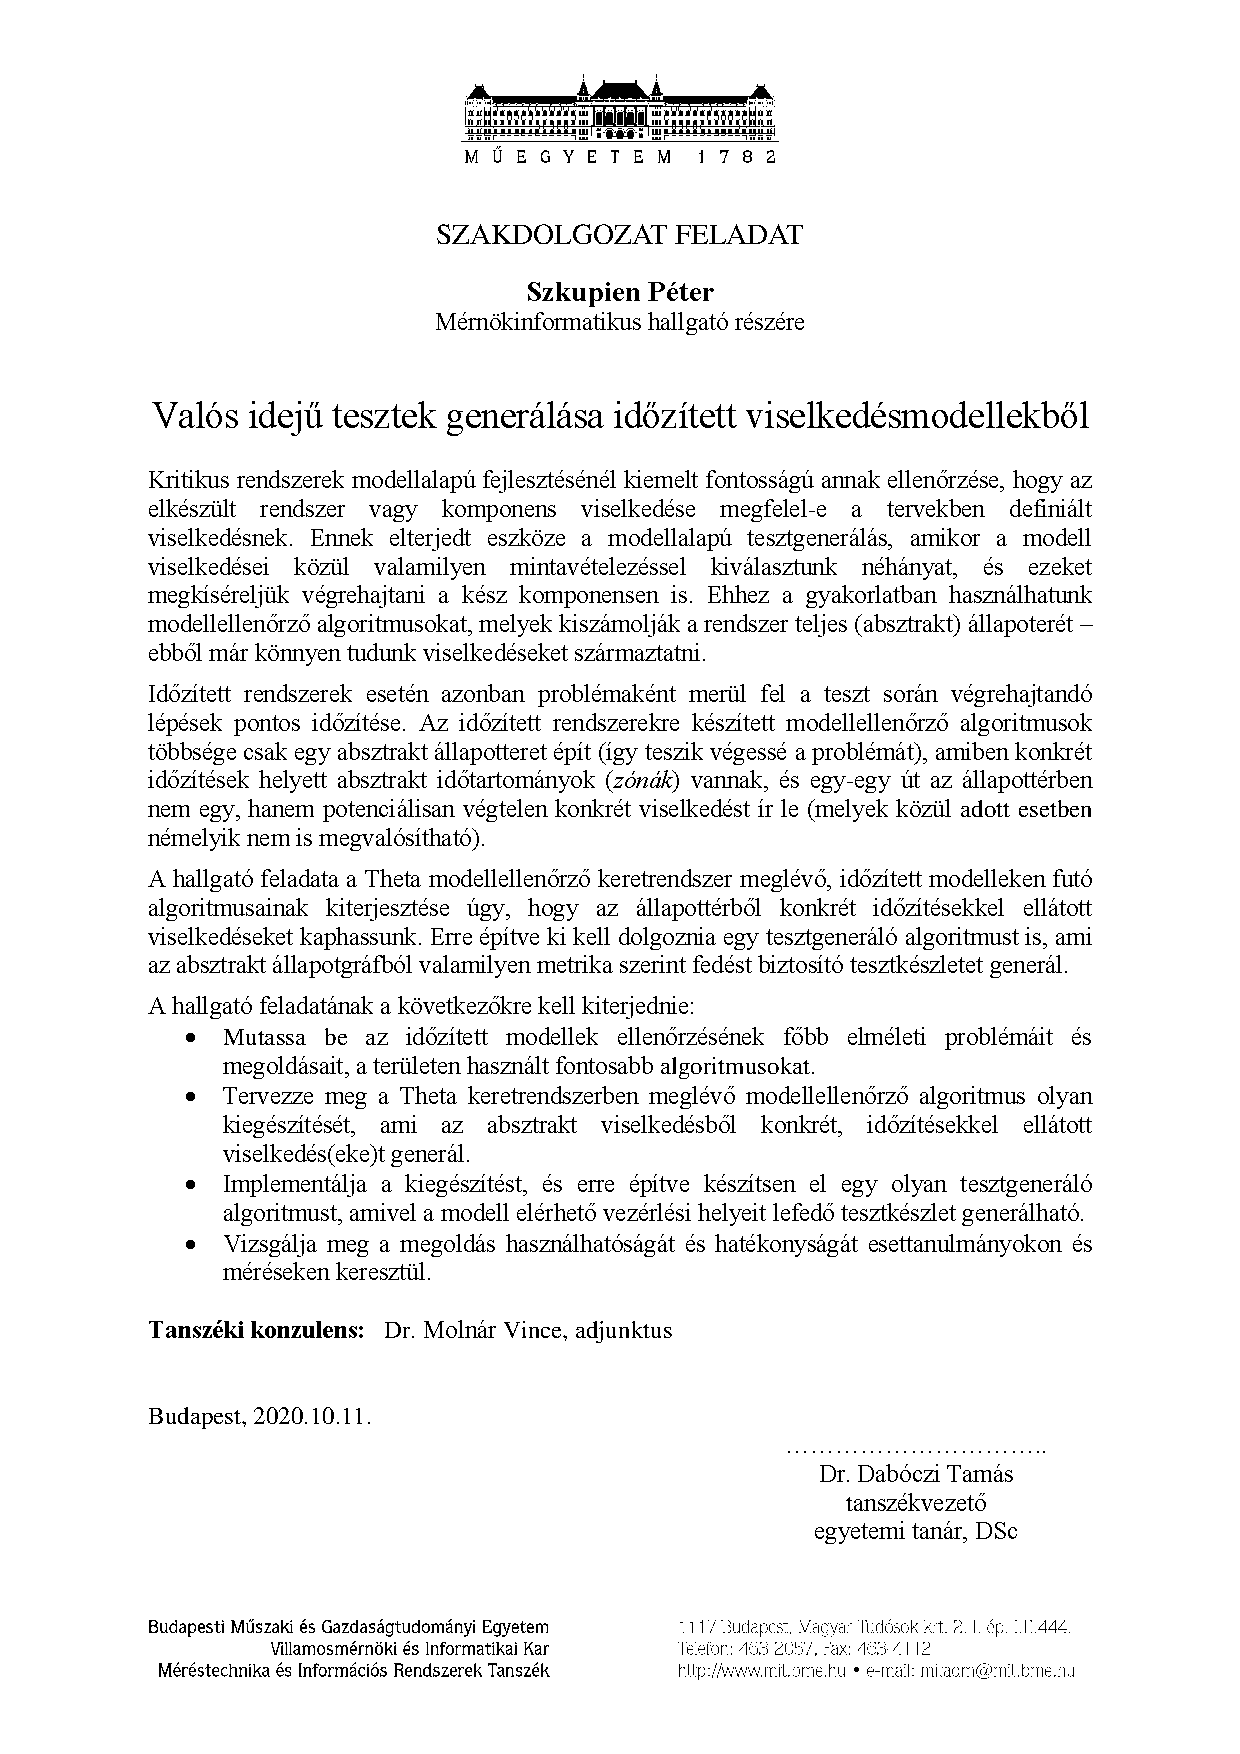
\includepdf[pages=-]{src/include/feladatkiiras.pdf}
     %Feladatkiírás

\hypersetup{pageanchor=false}
%--------------------------------------------------------------------------------------
%	The title page
%--------------------------------------------------------------------------------------
\begin{titlepage}
\begin{center}

\includegraphics[width=60mm,keepaspectratio]{figures/bme_logo.pdf}\\
\vspace{0.3cm}
\textbf{\bme}\\
\textmd{\vik}\\
\textmd{\viktanszek}\\[5cm]

\vspace{0.4cm}
{\huge \bfseries \vikcim}\\[0.8cm]
\vspace{0.5cm}
\textsc{\Large \vikdoktipus}\\[4cm]

{
	\renewcommand{\arraystretch}{0.85}
	\begin{tabular}{cc}
	 \makebox[7cm]{\emph{\keszitette}} & \makebox[7cm]{\emph{\konzulens}} \\ \noalign{\smallskip}
	 \makebox[7cm]{\szerzo} & \makebox[7cm]{\vikkonzulensA} \\
	  & \makebox[7cm]{\vikkonzulensB} \\
	  & \makebox[7cm]{\vikkonzulensC} \\
	\end{tabular}
}

\vfill
{\large \today}
\end{center}
\end{titlepage}
\hypersetup{pageanchor=false}

		   % Szakdolgozat/Diplomaterv címlap

\selectlanguage{magyar}
\pagenumbering{gobble}
%--------------------------------------------------------------------------------------
% Nyilatkozat
%--------------------------------------------------------------------------------------
\begin{center}
\large
\textbf{HALLGATÓI NYILATKOZAT}\\
\end{center}

Alulírott \emph{\vikszerzoVezeteknev{} \vikszerzoKeresztnev}, szigorló hallgató kijelentem, hogy ezt a \vikmunkatipusat{} meg nem engedett segítség nélkül, saját magam készítettem, csak a megadott forrásokat (szakirodalom, eszközök stb.) használtam fel. Minden olyan részt, melyet szó szerint, vagy azonos értelemben, de átfogalmazva más forrásból átvettem, egyértelműen, a forrás megadásával megjelöltem.

Hozzájárulok, hogy a jelen munkám alapadatait (szerző(k), cím, angol és magyar nyelvű tartalmi kivonat, készítés éve, konzulens(ek) neve) a BME VIK nyilvánosan hozzáférhető elektronikus formában, a munka teljes szövegét pedig az egyetem belső hálózatán keresztül (vagy autentikált felhasználók számára) közzétegye. Kijelentem, hogy a benyújtott munka és annak elektronikus verziója megegyezik. Dékáni engedéllyel titkosított diplomatervek esetén a dolgozat szövege csak 3 év eltelte után válik hozzáférhetővé.

\begin{flushleft}
\vspace*{1cm}
Budapest, \today
\end{flushleft}

\begin{flushright}
 \vspace*{1cm}
 \makebox[7cm]{\rule{6cm}{.4pt}}\\
 \makebox[7cm]{\emph{\vikszerzoVezeteknev{} \vikszerzoKeresztnev}}\\
 \makebox[7cm]{hallgató}
\end{flushright}
\thispagestyle{empty}

\vfill
\cleardoublepage

\selectthesislanguage
 %Hallgatói nyilatkozat

% Table of Contents
%~~~~~~~~~~~~~~~~~~~~~~~~~~~~~~~~~~~~~~~~~~~~~~~~~~~~~~~~~~~~~~~~~~~~~~~~~~~~~~~~~~~~~~
\tableofcontents\cleardoublepage


% Declaration and Abstract
%~~~~~~~~~~~~~~~~~~~~~~~~~~~~~~~~~~~~~~~~~~~~~~~~~~~~~~~~~~~~~~~~~~~~~~~~~~~~~~~~~~~~~~

% TeXstudio spellcheck 2020-12-10 16:25

\pagenumbering{roman}
\setcounter{page}{1}

\selecthungarian

%----------------------------------------------------------------------------
% Abstract in Hungarian
%----------------------------------------------------------------------------
\chapter*{Kivonat}\addcontentsline{toc}{chapter}{Kivonat}

Napjainkban már szinte minden biztonságkritikus rendszert szoftverek vezérelnek, amelyeknek minden körülmények között helyesen kell működniük, ellenkező esetben beláthatatlan következményekkel kellene szembenéznünk. A helyességbizonyítás elengedhetetlen alapja a rendszer és a biztonsági követelmények formalizálása. Noha a rendszerek helyességének bizonyítására egyre gyakrabban formális módszereket alkalmaznak, ez önmagában nem helyettesíti bizonyos konkrét tesztesetek lefuttatását.

A tesztkészletekkel szemben általános elvárás, hogy a rendszer minél több működését lefedjék, amire a modellalapú tesztgenerálás nyújt megoldást. Ekkor a teszteseteket nem kézzel adjuk meg, hanem a rendszer viselkedésmodelljének bejárásával generáljuk. Időzített rendszerek esetén azonban a tesztgenerálás összetettebb feladat: nem elegendő megadni a rendszer egy állapotsorozatát, az állapotváltozásokhoz konkrét időzítéseket is kell rendelnünk ahhoz, hogy megkapjuk a rendszer egy valós idejű tesztjét.

Szakdolgozatomban áttekintem a modellellenőrzés alapjait és az időzített viselkedésmodellek elméletét, valamint az időzített automatákon alkalmazható absztrakciókat és az SMT problémát. Formalizálom az időzített tesztekkel kapcsolatos fogalmakat és elvárásokat, valamint bemutatok egy algoritmust, amely a rendszer egy absztrakt modelljéből minden elérhető vezérlési helyét fedő tesztkészletet generál. Az absztrakt modell bejárásával kapott absztrakt tesztesetek időzítését visszavezetem SMT problémákra.

Bemutatom a Theta modellellenőrző keretrendszer releváns komponenseit, majd azokat kiegészítve implementálom az algoritmust, melyet végül esettanulmányon és méréseken keresztül részletesen is bemutatok.

\vfill
\selectenglish


%----------------------------------------------------------------------------
% Abstract in English
%----------------------------------------------------------------------------
\chapter*{Abstract}\addcontentsline{toc}{chapter}{Abstract}

Nowadays almost all safety critical systems are controlled by software which must operate correctly under all circumstances, otherwise we face unforeseeable consequences. Formalizing the system and its requirements is an essential base of proving correctness. Although formal methods are used more and more often in order to prove the correctness of systems, they do not, on their own, replace running certain test cases.

It is a general expectation towards test sets that they cover as many use cases as possible, which can be achieved by model-based test generation—generating test cases by traversing the behavioral model of the system instead of defining them manually. For timed systems, however, test generation becomes more complex as it is not enough to define a state sequence of the system but timing also has to be mapped to transitions to obtain a real-time test case.

In this thesis, the basics of model checking, theory of timed behavioral models, as well as applicable abstractions of timed automata and the SMT problem are presented. The concepts and expectations of real-time tests are formalized and an algorithm is presented which, using an abstract model of the system, generates a test set covering every available location of the system. The timing of the abstract test cases obtained from the traversal of the abstract model is reduced to SMT problems.

The relevant parts of the model checking framework Theta are also presented and the algorithm is implemented as their extension. Finally, the algorithm is discussed in detail through a case study and measurements.

\vfill
\cleardoublepage

\selectthesislanguage

\newcounter{romanPage}
\setcounter{romanPage}{\value{page}}
\stepcounter{romanPage}    %Összefoglaló


% The main part of the thesis
%~~~~~~~~~~~~~~~~~~~~~~~~~~~~~~~~~~~~~~~~~~~~~~~~~~~~~~~~~~~~~~~~~~~~~~~~~~~~~~~~~~~~~~
\pagenumbering{arabic}

%import your own content
% TeXstudio spellcheck 2020-12-10 16:31

%----------------------------------------------------------------------------
\chapter{\bevezetes}
%----------------------------------------------------------------------------
%\vspace{-1cm}
Biztonságkritikus informatikai rendszerek esetében kiemelt fontosságú, hogy megbizonyosodhassunk arról, megfelel-e az elkészített rendszer azoknak a követelményeknek, amelyeket eredetileg támasztottak vele szemben. Ennek ellenkezője ugyanis beláthatatlan következményekkel járhat: gondoljunk például atomerőművek vezérlésére, autóbuszok fékjére, repülők hajtóművére. Egy elkészült szoftverrendszer ellenőrzésének egyik módszere a tesztelés: annak vizsgálata, hogy a rendszer bizonyos bemenetekre (tesztesetekre) hogyan viselkedik, milyen állapotba kerül (\emph{white box test}), milyen kimenetet produkál (\emph{black box test}). Noha vannak ökölszabályok (pl. ekvivalencia-osztályok, határérték-analízis stb.) arra, hogy egy rendszer tesztelésekor milyen elvek mentén érdemes tesztbemeneteket választani ahhoz, hogy azok minél inkább lefedjék a rendszer lehetséges működéseit, ezek a kézzel megválasztott tesztesetek legfeljebb valószínűsíthetik a helyes működést, de nem alkalmasak arra, hogy egy rendszerről matematikai precizitással \emph{bizonyítsanak} valamit.

A megoldást a rendszer és a követelmények formalizálása jelenti, ami lehetővé teszi a modellek ellenőrzését formális módszerekkel. Ezek a módszerek matematikai alapokon nyugszanak, és a rendszer összes viselkedésének figyelembe vételével bizonyosodnak meg egy követelmény teljesüléséről vagy annak hiányáról. Nem elég azonban önmagában, ha egy algoritmus azt a kimenetet adja, hogy a rendszerünk nem teljesít egy követelményt, az is hasznos, ha ilyenkor megkapjuk a rendszer egy konkrét lefutását, amely egy olyan állapotba vezet, ahol a követelmény ténylegesen sérül – megkönnyítve ezzel a hiba javítását.

Nemcsak a követelmények sérülésekor hasznos a konkrét lefutások generálása: \emph{modellalapú tesztgenerálás} esetén a modellellenőrzés során feltárt teljes állapottér felhasználásával generálunk olyan tesztkészletet, amely lefedi a rendszer minél több (bizonyos metrika szerint akár összes releváns) működését. Ennek a jelentőségét az adja, hogy hiába tudjuk egy formális modellről biztosan, hogy teljesít egy követelményt, az implementáció során is kerülhetnek hibák a rendszerbe, amelyeket már valóban csak tesztekkel (a rendszer konkrét futtatásával) lehet kiszűrni. Éppen ezért hasznos, ha az elméletben helyes rendszer tényleges megvalósítása után is le tudjuk ellenőrizni, hogy teljesülnek-e a követelmények -- ha nem, akkor valójában nem a formális modell által leírt rendszert valósítottuk meg.

Időzített rendszerek esetén a teljes állapottér gyakran végtelen, így annak (minél nagyobb arányú) bejárása csak absztrakció segítségével lehetséges. Az állapotok absztrahálásával egy olyan absztrakt állapottérre egyszerűsítjük a feladatot, amely már véges, így kezelhető. Egy absztrakt állapottérben egy út azonban nem egy konkrét viselkedést (tesztesetet) ír le, hanem akár végtelen sokat.

Ha a modellellenőrző algoritmus talál egy utat az absztrakt állapottérben, az út menti állapotváltozásokhoz még konkrét időzítést is generálnunk kell. Ennek az időzítésnek pedig olyannak kell lennie, hogy az általa kapott konkrét út (teszteset) valóban abba az absztrakt útba (tesztesetbe) tartozzon, amit a modellellenőrző algoritmus eredetileg talált. Ezt az biztosítja, ha a konkrét útra teljesül minden olyan feltétel, amivel a modellellenőrző algoritmus az absztrakt utat specifikálta.

Az időzített automaták területének megkerülhetetlen eszköze az UPPAAL \cite{UPPAAL}. Az első kiadás 1995-ös dátuma is mutatja, hogy a probléma valós és régóta fennáll. Az UPPAAL-ban időzített automaták hálózatait modellezhetjük, vagyis nem pusztán az automatákat, de az azok közti kommunikációt is. Ezen rendszerekre megfogalmazhatunk feltételeket, amelyek teljesülését az UPPAAL modellellenőrzője ellenőrzi, azok sérülése esetén pedig ún. \emph{diagnostic trace}-t ad vissza, amely a rendszerünk egy olyan konkrét lefutása, amely abba az állapotba vezet, ahol a feltétel sérül. Ezeket a trace-eket szimulálhatjuk is. Az is megadható, hogy egy feltétel sérülése esetén milyen trace-t szeretnénk kapni: választhatjuk a \emph{legrövidebbet} (lépésszámban) vagy a \emph{leggyorsabbat} (időben) is.

A Theta \cite{Theta} modellellenőrző keretrendszert a Budapesti Műszaki és Gazdaságtudományi Egyetem Méréstechnika és Információs Rendszerek Tanszékén fejlesztik. Előnye, hogy több formalizmuson is működik, és felépítéséből adódóan könnyedén bővíthető továbbiakkal is. A modellellenőrző magja absztrakciót használ, amely hatékony működést eredményez.

Szakdolgozatomban a Theta modellellenőrző keretrendszer kiegészítését mutatom be: egy időzített automata absztrakt reprezentációjából olyan konkrét tesztesetek (időzített lépéssorozatok) generálását, amelyek \emph{lefedik a modell összes vezérlési helyét}.

A tesztesetek milyenségét illetően az UPPAAL-ban megismert célok (legrövidebb, leggyorsabb) itt is relevánsak, azonban nemcsak a tesztesetekre, hanem a teljes tesztkészletre vonatkozóan is értelmezhetők hasonló metrikák.

A fejlesztés távlatibb célja egy olyan folyamat támogatása, amelynek bemenete egy időzített mérnöki modell (pl. egy SysML állapotgép Magic Draw-ból\footnote{\url{https://www.nomagic.com/products/magicdraw}}), kimenete pedig egy (adott követelményeknek megfelelő) tesztkészlet. Ennek a folyamatnak a köztes lépése a szintén a Budapesti Műszaki és Gazdaságtudományi Egyetem Méréstechnika és Információs Rendszerek Tanszékén fejlesztett Gamma \cite{Gamma} eszköz segítségével történik, amely magas szintű mérnöki modelleket képes alacsonyabb szintű formális reprezentációkra (esetünkben pl. időzített automaták hálózatára) leképezni. A Gamma által előállított időzített automatákon futna tehát a Theta modellellenőrzője és tesztgenerálása. Ez a komplex tesztgenerálási folyamat komoly előrelépés lenne az időzített biztonságkritikus rendszerek fejlesztésében.

Szakdolgozatom \ref{hatterismeretek}. fejezetében áttekintem a témához kapcsolódó háttérismereteket: a modellek és követelmények formalizálását, valamint a modellellenőrzés elméletét. Bemutatom az időzített modellek formális leírását, annak szintaktikáját és szemantikáját, valamint, hogy milyen absztrakcióval tehető végessé a kezdetben végtelen állapottér, milyen adatstruktúrával írható le a véges, absztrakt modell. Áttekintem a kényszerkielégíthetőségi problémák leírását és ezek megoldását, majd bemutatom a Theta modellellenőrző keretrendszert. A \ref{main-elmelet}. fejezetben formalizálom a feladatot, és részletesen bemutatom az általam megvalósított tesztgeneráló algoritmust, majd a \ref{main-gyakorlat}. fejezetben annak implementációját is áttekintem. Az \ref{esettanulmany}. fejezetben egy esettanulmányon keresztül bemutatom a teljes tesztgenerálási folyamatot, majd áttekintem az implementációm mérési eredményeit. Végül a \ref{osszefoglalas}. fejezetben összefoglalom a munkámat és sorra veszem a megoldásom továbbfejlesztési lehetőségeit.
% TeXstudio spellcheck 2020-12-10 16:30

\chapter{Háttérismeretek} \label{hatterismeretek}

Ebben a fejezetben összefoglalom a szakdolgozat témájához kapcsolódó háttérismereteket. Bemutatom a modellellenőrzés alapjait (\ref{modellellenorzes}. fejezet), az időzített automaták elméletét és absztrakciós módszereit (\ref{idozitett-automata}. fejezet), az SMT problémákat (\ref{smt}. fejezet), valamint a Theta modellellenőrző keretrendszert (\ref{theta}. fejezet).

\section{Modellellenőrzés} \label{modellellenorzes}

A modellellenőrzés \cite{IntroductionToModelChecking} egy algoritmikus módszer tranzíciós rendszerek dinamikus viselkedésének vizsgálatára. A modellellenőrzéshez (\ref{fig:modell-ell} ábra) alapvetően három dolog szükséges:
\begin{itemize}
    \item \textbf{Formális modell}: Az állapotokat és tranzíciókat tartalmazó véges gráfokkal jól modellezhetők a véges állapotú rendszerek. Esetünkben az időzített automata formalizmussal fogjuk leírni a rendszereket.
    \item \textbf{Formális követelmény}: A modellre vonatkozó általánosabb követelmények megfogalmazhatók pl. temporális logikák \cite{IntroductionToModelChecking} segítségével, ám ezeket szakdolgozatomban nem részletezem. Esetünkben a vezérlési helyek elérhetősége fogja specifikálni a rendszert, ami felírható egy biztonsági követelmény negáltjaként is (a vizsgált invariáns a keresett vezérlési hely elérhetetlensége lesz).
    \item \textbf{Algoritmus}: Szükséges egy olyan algoritmus, amely a modellről eldönti, hogy teljesíti-e a specifikációban foglalt követelményeket.
\end{itemize}

A modellek pontos verifikációja gyakran már kis rendszerek esetében is komoly kihívást jelent, ám teljes bizonyítás nélkül is lehet hasznos a modellellenőrzés hibák felderítésére.

\begin{figure}
    \centering
    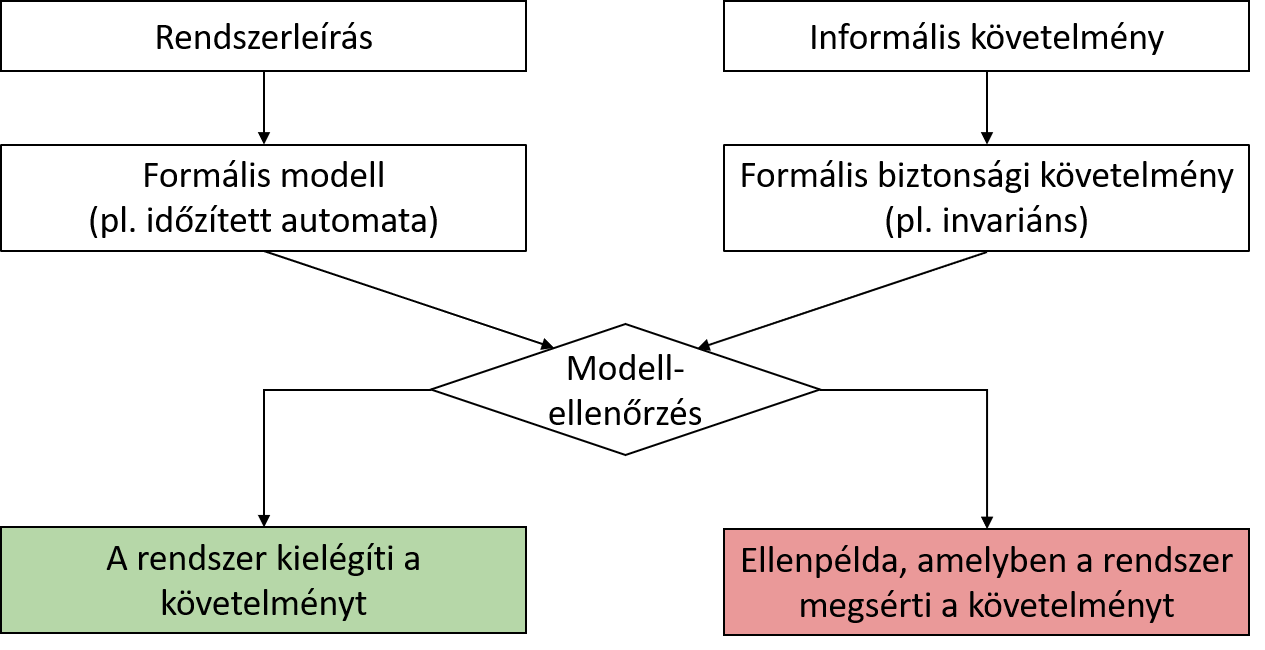
\includegraphics[width=0.85\textwidth, keepaspectratio]{figures/modellell.png}
    \caption{Modellellenőrzés}
    \label{fig:modell-ell}
\end{figure}

%\newpage
A véges állapotú rendszerek formális leírására az egyik legegyszerűbb formalizmus a \emph{Kripke-struktúra} \cite{IntroductionToModelChecking}.

\begin{definition}[Kripke-struktúra]
Egy $K$ \emph{Kripke-struktúra} egy irányított gráf, amelynek csúcsai $A$ atomi tulajdonságok egy-egy részhalmazával vannak címkézve. Formálisan $K = \langle S, R, L \rangle$, ahol
\begin{itemize}
    \item $S$ az állapotok halmaza (az állapottér),
    \item $R \subseteq S \times S$ a tranzíciók halmaza,
    \item $L: S \rightarrow 2^A$ a címkézőfüggvény, amely minden állapothoz az atomi tulajdonságok egy halmazát rendeli.
\end{itemize}
Egy Kripke-struktúra véges, ha $S$ véges.
\end{definition}

Egy $K$ \emph{Kripke-struktúra} $s \in S$ állapotára jelölje $L(s)$ azon atomi tulajdonságok halmazát, amelyek teljesülnek, ha a $K$ rendszer $s$ állapotban van, $A \setminus L(s)$ pedig azon atomi tulajdonságok halmazát, amelyek ugyanekkor nem teljesülnek.

%A \emph{tesztelés} a hibák megtalálásának leggyorsabb és legegyszerűbb módja. Teszteléssel azonban csak megtalálni lehet a hibákat, azok hiányát nem lehet hitelt érdemlően bizonyítani.

\subsection{A modellellenőrzés előnyei és kihívásai}

A modellellenőrzésnek több előnye is van, amely megkülönbözteti más módszerektől, így a teszteléstől is \cite{IntroductionToModelChecking}.
\begin{enumerate}
    \item Egyrészt ez egy algoritmikus módszer, amely automatizálható (szemben a tesztekkel, amelyeket kézzel meg kell írni).
    \item Másrészt a modellellenőrzés a rendszer létrejöttének bármelyik szintjén alkalmazható, vagyis már a tervezés fázisában is ellenőrizhető a rendszer (szemben a teszteléssel, hiszen egy teszt lefuttatása nem lehetséges egy még nem implementált rendszeren).
    \item Harmadrészt a modellellenőrzés konkurens rendszerek vizsgálatára is alkalmas. Ez különösen fontos, hiszen rohamosan terjednek a többprocesszoros rendszerek, a konkurens működés viszont a hibák jelentős hányadát is adja. Ezeket a hibákat viszont teszteléssel nagyon nehéz detektálni, reprodukálni.
\end{enumerate}

A rendszer változóinak számától akár exponenciálisan függhet az állapotok száma (\emph{állapottér-robbanás}), de bizonyos esetekben (pl. valamilyen felső korlát hiánya) akár végtelen is lehet az állapottér. A hatékony, való életbeli rendszereken is alkalmazható modellellenőrzés két kihívást is magában foglal.

\begin{itemize}
    \item Az \emph{algoritmikus kihívás} az algoritmus skálázódására vonatkozik. A nagy állapotterek hatékony kezelése kulcsfontosságú ahhoz, hogy valós méretű rendszereken is alkalmazható legyen az algoritmus.
    \item A \emph{modellezési kihívás} a bonyolult rendszerek formális modelljeinek lekicsinyítését, végessé tételét jelenti pl. absztrakció használatával.
\end{itemize}

A két kihívás természetesen összefügg, a megoldások közösen fejlődnek, hiszen önmagban egyik sem jelent használható módszert.

\subsection{Az állapottér-robbanás kezelése} \label{allapotterRobbanas}

Az állapottér-robbanás kezelése azt jelenti a modellellenőrzés során, hogy megpróbáljuk elkerülni, hogy explicit módon építsük fel és vizsgáljuk a rendszert leíró teljes Kripke-struktúrát (állapotteret). Az ezt célzó módszereket három csoportba sorolhatjuk \cite{IntroductionToModelChecking}.
\begin{itemize}
    \item A \textbf{strukturális módszerek} a rendszer felépítésének (struktúrájának) sajátosságait (pl. szimmetria, rekurzió) használják fel az állapottér kezelésére.
    \item A \textbf{szimbolikus technikák} az állapotok és tranzíciók halmazait valamilyen szimbolikus logikai kifejezéssel írják le (pl. bináris döntési diagram), ezzel tömörítve a teljes rendszer leírását is.
    \item Az \textbf{absztrakció} az eredeti Kripke-struktúra redukálását jelenti egy kisebbre úgy, hogy az is megtartsa az eredetinek bizonyos tulajdonságait.
\end{itemize}

\emph{Absztrakció} használatakor tehát a rendszert leíró $K$ Kripke-struktúrát egy kisebb $\hat{K}$ Kripke-struktúrára (absztrakt modellre) redukáljuk a hatékonyabb feldolgozás érdekében ($\hat{K}$ tehát felülbecslése, elnagyolása $K$-nak). Fontos, hogy az ellenőrizendő követelményünk szempontjából releváns tulajdonságokat nem nagyolhatunk el az absztrakció során, hiszen csak így biztosítható, hogy $\hat{K}$ csak azokat a követelményeket teljesítse, amelyeket $K$ is teljesít.

Jelöljön $\varphi$ egy $K$-n ellenőrizhető követelményt, $K \models \varphi$ pedig azt, ha $K$ teljesíti $\varphi$-t. Formálisan ha $\hat{K}$ szimulálja $K$-t, akkor bármely vizsgált $\varphi$-re ha $\hat{K} \models \varphi$, akkor $K \models \varphi$.

Az \emph{ellenpélda-vezérelt absztrakciófinomítás} \cite{IntroductionToModelChecking} (\ref{fig:cegar} ábra) során iterációnként tovább finomítjuk a $\hat{K}$ absztrakciót, amennyiben ez szükséges.
\begin{itemize}
    \item Ha az absztrakt $\hat{K}$ modell teljesíti a $\varphi$ követelményt, az eredeti $K$ modell is biztosan teljesíti azt (hiszen $\hat{K}$ akkor szimulálja $K$-t (vagyis akkor megfelelő az absztrakció), ha bármely vizsgált $\varphi$-re $\hat{K} \models \varphi \Rightarrow K \models \varphi$).
    \item Ha az absztrakt $\hat{K}$ modell nem teljesíti $\varphi$-t ($\hat{K} \not \models \varphi$), a kapott $\hat{\pi}$ absztrakt ellenpéldát megpróbáljuk konkretizálni.
    \begin{itemize}
        \item Amennyiben ez sikerül, vagyis a $\hat{\pi}$ ellenpélda valódi, az eredeti $K$ rendszer sem teljesíti $\varphi$-t ($K \not \models \varphi$).
        \item Amennyiben a $\hat{\pi}$ ellenpéldát nem sikerül konkretizálni, mert az nem valódi (vagyis csak az absztrakció miatt találhattuk meg), az absztrakt $\hat{K}$-t tovább kell finomítanunk, hogy már ne találhassuk meg benne újra ezt a hamis $\hat{\pi}$ ellenpéldát.
    \end{itemize}
\end{itemize}

\begin{figure}
    \centering
    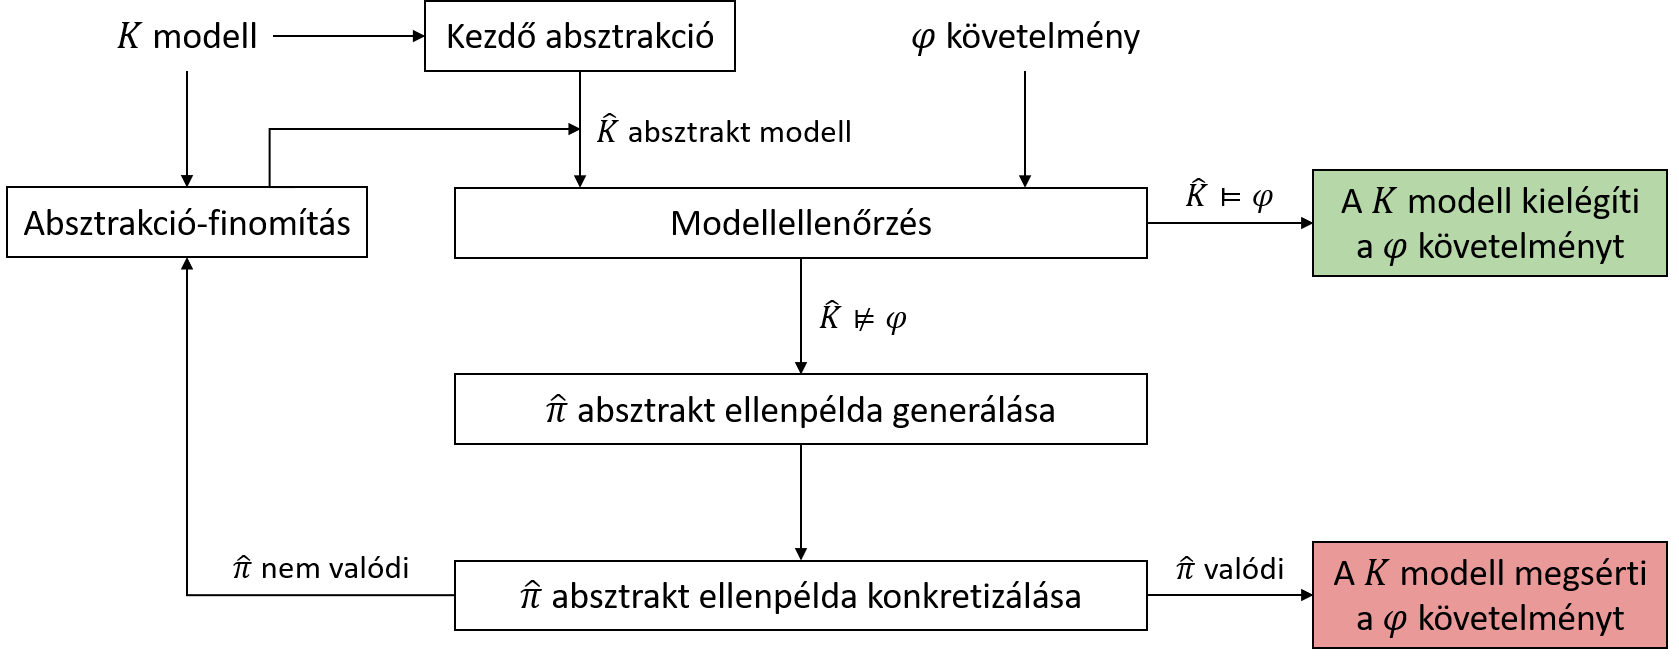
\includegraphics[width=\textwidth, keepaspectratio]{figures/cegar.png}
    \caption{Ellenpélda-vezérelt absztrakciófinomítás}
    \label{fig:cegar}
\end{figure}

\section{Időzített automata} \label{idozitett-automata}

Az időfüggő viselkedésű rendszerek leírására az időzített automata \cite{TimedAutomata} formalizmust alkalmazhatjuk. Az időzített automaták óraváltozókkal kiegészített véges automaták. Az óraváltozók olyan speciális változók, amelyek értéke

\begin{itemize}
    \item valós ($x\in\mathbb{R}$),
    \item 0-ról indul ($x_0=0$),
    \item az automata működése során növekszik (vagyis $x\geq0$),
    \item lenullázható.
\end{itemize}

Jelölje az $x$, $y$ stb. óraváltozók halmazát $\mathcal{C}$, az $a$, $b$ stb. akciók ábécéjét $\Sigma$, az üres akciót $\varepsilon$. Az óraváltozókra ($x \sim n$) vagy azok különbségeire ($x - y \sim n$) megfogalmazhatunk kényszereket (ahol $x$ és $y$ óraváltozók, $\sim$ relációs jel, valamint $n \in \mathbb{N}_0^+$). $\mathcal{B}(\mathcal{C})$-vel jelöljük $\mathcal{C}$-beli óraváltozókra vonatkozó összes lehetséges kényszer halmazát.

\begin{definition}[Időzített automata]
\label{IdőzítettAutomata}
Egy $\mathcal{A}$ \emph{időzített automata} formálisan $\langle L,l_0,T,I\rangle$, ahol
\begin{itemize}
    \item $L$ a vezérlési helyek véges halmaza,
    \item $l_0 \in L$ a kezdő vezérlési hely,
    \item $T \subseteq L \times G \times \Sigma \times 2^\mathcal{C} \times L$ az élek halmaza, ahol $G \subseteq \mathcal{B}(\mathcal{C})$
    \item $I: L \rightarrow 2^{\mathcal{B}(\mathcal{C})}$ a vezérlési helyekhez tartozó invariánsok.
\end{itemize}
\end{definition}

\begin{figure}
    \centering
    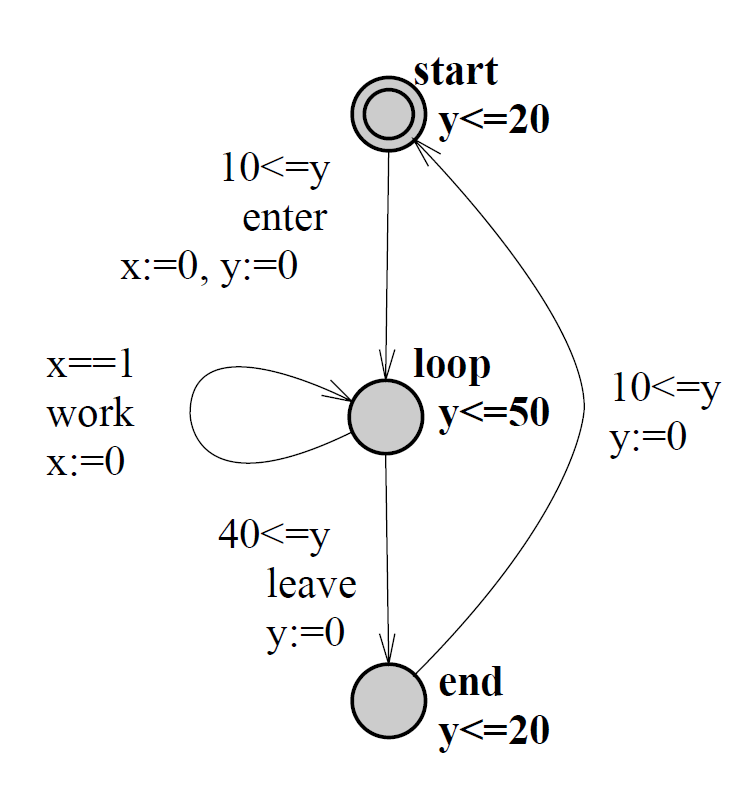
\includegraphics[height=60mm, keepaspectratio]{figures/idozitett-automata-pelda.png}
    \caption{Időzített automata \cite{TimedAutomata}}
    \label{fig:idozitett-automata-pelda}
\end{figure}

\begin{example}[Időzített automata]
A \ref{fig:idozitett-automata-pelda} ábrán látható időzített automata bemeneti ábécéje $\Sigma = \{enter, work, leave\}$, formális leírása $\mathcal{A}^1 = \langle L^1,l_0^1,T^1,I^1 \rangle$, ahol
\begin{itemize}
    \item $L^1 = \{start, loop, end\}$,
    \item $l_0^1 = start$,
    \item $T^1 = 
    \begin{Bmatrix}
    (&start,& \{10 \leq y\},& enter,& \{x, y\},& loop&),\\
    (&loop,& \{x = 1\},& work,& \{x\},& loop&),\\
    (&loop,& \{40 \leq y\},& leave,& \{y\},& end&),\\
    (&end,& \{10 \leq y\},& \varepsilon,& \{y\},& start&)
    \end{Bmatrix}$,
    \item $I^1 = \{ (start \rightarrow \{ y \leq 20 \}), (loop \rightarrow \{ y \leq 50 \}), (end \rightarrow \{ y \leq 20 \}) \}$.
\end{itemize}
\end{example}

Egy $t \in T$ él egy $L$-beli vezérlési helyből egy $L$-beli vezérlési helybe vezet, adott $\mathcal{B}(\mathcal{C})$-beli $G$ őrfeltételek mellett, valamely $\Sigma$-beli akció hatására, a $\mathcal{C}$-beli óraváltozók egy részhalmazának lenullázásával.
Óraváltozókat három módon használhatunk időzített automatákban (ezek mindegyikére mutat példát a \ref{fig:idozitett-automata-pelda} ábra).

\begin{itemize}
    \item 	\textbf{Őrfeltétel élen}: az él csak akkor tüzelhet, ha az őrfeltétel teljesül. A példában a $start$ vezérlési helyről csak akkor léphetünk át a $loop$ vezérlési helyre, ha a $10 \leq y$ feltétel teljesül.
    \item 	\textbf{Lenullázás éllel}: ha az él tüzel, az óraváltozó értéke $0$ lesz. A példában ha az automata az $end$ vezérlési helyről a $start$ vezérlési helyre lép, az $y$ óraváltozó értéke lenullázódik.
    \item 	\textbf{Vezérlési hely invariáns}: az automata csak olyan vezérlési helyen lehet, amelynek az összes invariáns feltétele teljesül. A példában mivel az $end$ vezérlési helyhez az $y \leq 20$ invariáns tartozik, az automatának el kell hagynia az $end$ vezérlési helyet legkésőbb, amikor $y$ értéke $20$ lesz.
\end{itemize}

Jelölje $u$ az óraváltozók egy állását, vagyis egy olyan $\mathcal{C} \rightarrow \mathbb{R}_+$ függvényt, amely értéket rendel minden óraváltozóhoz, $u(x)$ pedig az $x$ óraváltozó értékét az $u$ állásban. Szemantikáját tekintve egy időzített automata egy olyan \emph{Kripke-struktúra}, amelynek állapotai $\langle l, u \rangle$ párok, ahol $l$ egy vezérlési hely, $u$ pedig az óraváltozók egy állása, a címkéző függvény pedig minden állapothoz hozzárendeli az összes ott igaz állítást. A rendszerben kétféle tranzíció (állapotátmenet) lehetséges:
\begin{itemize}
    \item $\langle l, u \rangle \rightarrow \langle l, u + d \rangle$ esetben az automata az $l$ vezérlési helyen várakozik $d$ ideig. Ez értelemszerűen csak akkor lehetséges, ha az $l$ vezérlési helyhez tartozó invariánsokat $u + d$ is kielégíti.
    \item $\langle l, u \rangle \rightarrow \langle l', u' \rangle$ esetben az automata vezérlési helyet vált, $l$-ből $l$'-be lép át. Ez értelemszerűen csak akkor lehetséges, ha van tüzelhető él $l$-ből $l'$-be. Ekkor $u = u'$, kivéve az él által lenullázott óraváltozókat.
\end{itemize}
Egy időzített automata esetében a klasszikus verifikációs probléma az elérhetőség analízis \cite{RealTimeModelChecking}. A megválaszolandó kérdés tehát az, hogy egy $\langle l_0, u_0 \rangle$ kezdőállapotból egy adott $\langle l, u \rangle$ állapot elérhető-e.

Mivel az óraváltozók valós értékkészletű változók, végtelen sok értéket felvehetnek. Ráadásul egy rendszerben nemcsak egy, hanem több óraváltozó is lehet, vagyis egy időzített automata állapottere „többszörösen” végtelen. Adódik tehát az igény ennek az egyszerűsítésére, véges reprezentációjára. Erre több lehetőség is van: a folytonos időt feloszthatjuk régiókra vagy zónákra.

\subsection{Régió}
A valós értékkészletű óraváltozók okozta végtelen állapottér végessé tételének egyik lehetséges módja az idő (az óraváltozók értékkészleteinek) régiókra osztása. Ennél a módszernél azt használjuk ki, hogy az időzített automata működése hogyan függhet az óraváltozók értékeitől. Ha két $u, v$ óraváltozó-állás ugyan különbözik, de ez a különbség az automata működésében nem jelenik meg (és nem is jelenhet meg), tekinthetjük őket azonosnak. Az ezen gondolatmenet alapján azonosnak tekintett állások tartoznak egy régióba, tehát ez a legfinomabb felbontás, amire szükségünk lehet.
\begin{itemize}
    \item Minden $x \in \mathcal{C}$ óraváltozóhoz hozzárendeljük azt a legnagyobb $k(x)$ konstanst, amely rá vonatkozó feltételben szerepel a rendszerben. Az $x$ óraváltozó két $x_i > k(x)$, $x_j > k(x)$ értéke azonosnak tekinthető, hiszen nem lehet két olyan feltétel a rendszerben, amelyre más eredményt adnak.
    
    \item Az óraváltozókra megfogalmazott $x \sim n$ feltételekben $n \in \mathbb{N}_0^+$, vagyis az óraváltozók valós értékét mindig nemnegatív egészekkel hasonlítjuk össze. Az $x$ óraváltozó két $m \in \mathbb{N} < x_i, x_j < m + 1$ értéke tehát ebből a szempontból azonosnak tekinthető, hiszen nem lehet olyan $x \sim n$ feltétel a rendszerben, amelyre más eredményt adnak.
    
    \item Az óraváltozók különbségeire is megfogalmazhatunk kényszereket $x - y \sim n$ alakban, vagyis két $u, v$ óraváltozó-állás nem tekinthető azonosnak, ha van bennük két $x, y$ óra, amelyekre $u(x) \sim u(y)$ és $v(x) \sim v(y)$ $\sim$ relációja nem egyezik meg.
\end{itemize}

Egy példa $\mathcal{C} = \{x, y\}$ két óraváltozós rendszer régiói láthatók a \ref{fig:regiok-pelda} ábrán. A síknegyed vonalak által részben vagy egészben közrezárt területei és \emph{a szakaszok maguk is} külön régiók.

\begin{figure}
    \centering
    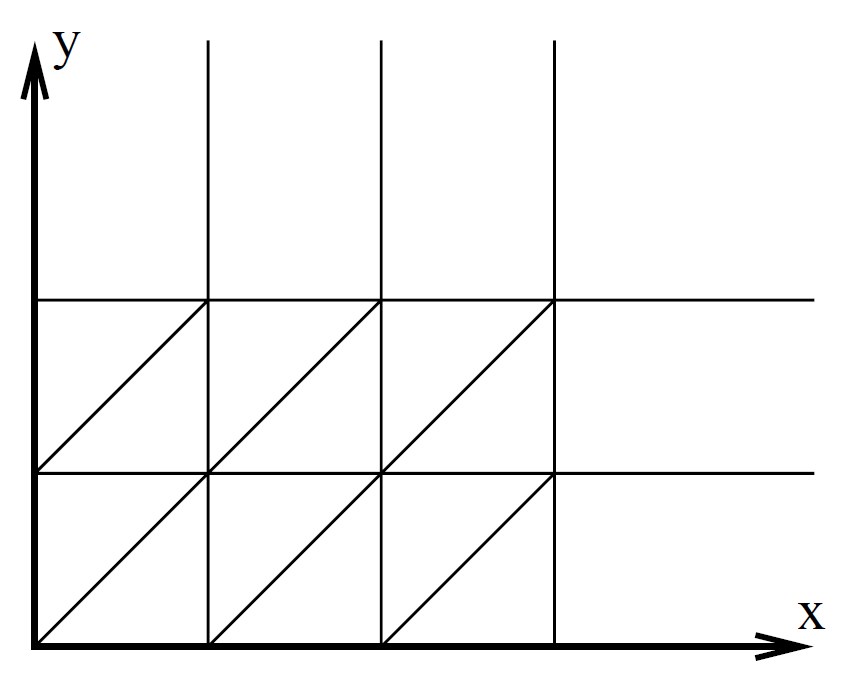
\includegraphics[height=60mm, keepaspectratio]{figures/regiok-pelda.png}
    \caption{Két óraváltozós rendszer régiói \cite{TimedAutomata}}
    \label{fig:regiok-pelda}
\end{figure}

\subsection{Zóna} \label{zona}
Általában nincs szükség a régiók adta granularitásra, ezért a gyakorlatban régiók egy konvex csoportjával dolgozunk: ezt hívjuk zónának.

\begin{definition}[Zóna]
Jelölje $\mathcal{C}$ az óraváltozók halmazát. Zónán a $\mathcal{C}$-beli óraváltozókra vonatkozó $C_i - C_j \sim n$ alakú kényszerek egy (konjunktív) halmazát értjük (ahol $\sim\ \in \{\leq,<,=,>,\geq\}$ és $n \in \mathbb{N}$), de zónának tekinthetjük azt a legtágabb óraváltozóérték-halmazt is, amely kielégíti a kényszerhalmazt.
\end{definition}

A korábban definiált $\langle l, u \rangle$ állapotok helyett bevezetünk $\langle l, \mathcal{Z} \rangle$ szimbolikus állapotokat, ahol $\mathcal{Z}$ egy zóna. A rendszerünk átmenetei ebben az esetben is a korábban leírtak szerint adódnak.

Szimbolikus állapotok alkalmazása esetén értelemszerűen az elérhetőség analízis is szimbolikus állapotokra értendő: a kérdés tehát az, hogy egy $\langle l_0, \mathcal{Z}_0 \rangle$ kezdőállapotból egy adott $\langle l, \mathcal{Z} \rangle$ szimbolikus állapot elérhető-e. Amennyiben $\langle l_f, \mathcal{Z}_f \rangle$-fel jelöljük a rendszer hibaállapotait (vagyis azokat az állapotokat, amelyek bizonyos biztonsági tulajdonságok, követelmények megsértését reprezentálják), a rendszerünk biztonságossága azt jelenti, hogy egyik $\langle l_f, \mathcal{Z}_f \rangle$ állapot sem érhető el.

A \ref{fig:zonagraf-pelda} ábra egy egyszerű időzített automatát és annak zónagráfját mutatja. Ránézésre is látható, hogy a zónagráf az időzített automatánk egy nagyon kompakt (elérhetőség szempontjából azonban teljes) reprezentációja. Hiába vehet fel az $x$ óraváltozó végtelen sok értéket, a zónagráfnak mindösszesen 8 csúcsa van. Látható, hogy a zónagráf csúcsai szimbolikus állapotok, vagyis vezérlési hely és zóna párok.

\begin{figure}
    \centering
    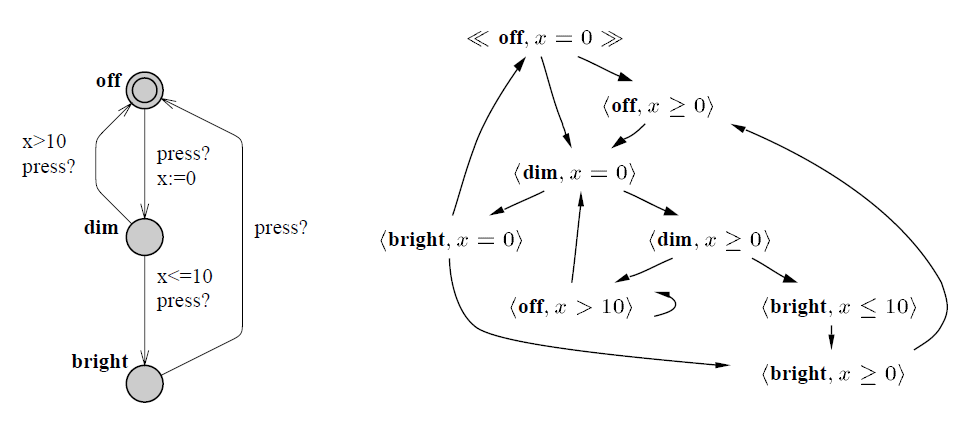
\includegraphics[width=\textwidth, keepaspectratio]{figures/zonagraf-pelda.png}
    \caption{Időzített automata zónagráfja \cite{TimedAutomata}}
    \label{fig:zonagraf-pelda}
\end{figure}

\subsection{Zónák mátrixos ábrázolása}
Az óraváltozókra vonatkozó kényszereknek két alakja lehetséges, ahol $x, y \in \mathcal{C}$, $\sim\ \in \{\leq,<,=,>,\geq\}$ és $n \in \mathbb{N}$. Egy kényszer vonatkozhat egy óraváltozó értékének és egy konstansnak a relációjára ($x \sim n$) vagy két óraváltozó különbségének és egy konstansnak a relációjára ($x-y \sim n$).

A kényszerek kezelése szempontjából kényelmetlen az előbb ismertetett két eltérő alak, ezért bevezetjük a \textbf{0} referenciaórát, amelynek értéke mindig 0. Ennek segítségével az $x \sim n$ alakú kényszerek $x-\textbf{0} \sim n$ alakúra hozhatók, vagyis az összes kényszert leírhatjuk $x-y \sim n$ alakban.

A \textbf{0} referenciaórával kiegészített órahalmazt jelölje $\mathcal{C}_0= \mathcal{C} \cup \{\textbf{0}\}$, az órákat pedig rendezzük sorrendbe, és jelölje az elemeket rendre $C_0,C_1,…,C_n$, ahol $C_0$ a referenciaóra, $C_1,…,C_n$ pedig az eredeti $\mathcal{C}$ órahalmaz.

A $\mathcal{C}_0$-beli óraváltozók különbségeire megfogalmazott kényszereket könnyen reprezentálhatjuk egy $(n+1) \times (n+1)$-es mátrixban, ezt az adatszerkezetet nevezzük \emph{Difference Bound Matrixnak} (DBM). A mátrix $(i,j)$ eleme ($0 \leq i, j \leq |\mathcal{C}|$) reprezentálja a (legszigorúbb) $C_i - C_j \sim n$ kényszert $(n, \sim)$ alakban. Amennyiben egy óraváltozópár különbségére nem vonatkozik kényszer, a mátrix megfelelő mezőjébe $\infty$ kerül.

\begin{example}[Difference Bound Matrix]
Vegyünk például egy rendszert két órával $\mathcal{C} = \{x, y\}$, majd egészítsük ki a \textbf{0} referenciaórával: $\mathcal{C}_0 = \mathcal{C} \cup \{ \textbf{0} \} = \{\textbf{0}, x, y\}$. Az óraváltozóink sorrendje ekkor legyen $C_0 = \textbf{0}, C_1 = x, C_2 = y$. Vegyük azt a $\mathcal{Z}$ zónát, amelyet az $x<20 \wedge y \leq 20 \wedge y-x \leq 10$ kényszerek írnak le. Az $x \sim n$ alakú kényszereket $x-y \sim n$ alakúra hozva a következő kifejezést kapjuk: $\mathcal{Z} = x-\textbf{0}<20 \wedge y-\textbf{0} \leq 20 \wedge y-x \leq 10$.

A $\mathcal{Z}$ zónához tartozó DBM a következő:

\[
M(\mathcal{Z}) = \begin{pmatrix}
(0,\leq) & (0,\leq) & (0,\leq)\\
(20,<) & (0,\leq) & \infty\\
(20,\leq) & (10,\leq) & (0,\leq)
\end{pmatrix}
\]
\end{example}

A $\mathcal{Z}$ zónát leíró $M(\mathcal{Z})$ DBM kapcsán a következő megfigyeléseket tehetjük:
\begin{itemize}
    \item A $\mathcal{Z}$ zónára vonatkozó kényszerek egyértelműen megjelennek az $M(\mathcal{Z})$ mátrixban. Az $x < 20$ ($x - \textbf{0} < 20$) kényszer a mátrix $(1,0)$ elemében $(20,<)$ alakban, az $y \leq 20$ ($y - \textbf{0} \leq 20$) kényszer a mátrix $(2,0)$ elemében $(20,\leq)$ alakban, míg az $y-x \leq 10$ kényszer a mátrix $(2,1)$ elemében $(10,\leq)$ alakban.
    \item A mátrix felső (nulladik) sorában kizárólag $(0,\leq)$ elemek szerepelnek, hiszen itt a $\textbf{0}$ referenciaóra és az óraváltozók negatív különbségeire vonatkozó „kényszerek” szerepelnek. Mivel $\textbf{0}$ értéke mindig 0, az óraváltozók értéke pedig biztosan nemnegatív, $\textbf{0}-C_i = 0-C_i$ értéke biztosan kisebb vagy egyenlő lesz 0-nál.
    \item A mátrix főátlójában is csak $(0,\leq)$ elemek szerepelnek. Ez is értelemszerű, hiszen itt az óraváltozók önmaguktól vett különbségére vonatkozó „kényszerek” állnak ($C_i - C_i \leq 0$).
    \item Mivel a $\mathcal{Z}$ zónában $x-y$-ra nem vonatkozik kényszer, a mátrix hozzá tartozó $(1,2)$ elemében $\infty$ szerepel.
\end{itemize}

A \ref{zona}. fejezetben bevezetett $\langle l, \mathcal{Z} \rangle$ alakú szimbolikus állapotok $\mathcal{Z}$ zónája tehát leírható egy DBM segítségével, vagyis egy szimbolikus állapotot egy vezérlési hely és egy DBM határoznak meg.

\subsection{Absztrakt állapottér-reprezentáció}
Az időzített automaták működésének leírására használhatjuk az Adaptive Simulation Graph (ASG) \cite{spin2018} adatszerkezetet, ez az adatstruktúra az absztrakcióhoz. Az ASG egy olyan gráf, amely az időzített automata (végtelen) lefutásait a (véges) gráfban lévő utakként reprezentálja.
\begin{definition}[Adaptive Simulation Graph]
\label{def:ASG}
Egy $\mathcal{A} = \langle L,l_0,T,I\rangle$ időzített automata $G$ ASG-je formálisan $\langle V, E, v_0, M_v, M_e, \rhd, \psi_Z, \psi_W \rangle$, ahol
\begin{itemize}
    \item $(V, E)$ egy irányított $v_0 \in V$ gyökerű fa gráf,
    \item $M_v: V \rightarrow L$ a csúcscímkézés,
    \item $M_e: E \rightarrow T$ az élcímkézés,
    \item $\rhd \subseteq V \times V$ a fedési reláció,
    \item $\psi_Z, \psi_W: V \rightarrow \{ \mathcal{Z}_i \}$ a csúcsok címkézése zónákkal.
\end{itemize}
\end{definition}

A csúcsok $\psi_Z$ zónacímkézése az állapothoz tartozó pontos zónát jelöli, míg $\psi_W$ ennek egy felülbecslése, absztrakciója. Az elérhetőség vizsgálata közben $\psi_Z$-t valójában nem tároljuk, az algoritmus a kezdetben durva felülbecslést fogja finomítani $\psi_W$-ben annyira, hogy a vizsgált követelmény belátható legyen.

A gráf $v$ csúcsai $\langle l, \mathcal{Z} \rangle$  szimbolikus állapotokat reprezentálnak, ahol $l=M_v(v), \mathcal{Z}=\psi_Z(v)$. A gráf csúcsaira értelmezett fedési reláció azt fejezi ki, hogy az egyik csúcs által reprezentált állapot része egy másik csúcs által reprezentáltnak. Formálisan $v,v' \in V$ csúcsokra $v \rhd v'$ esetén $M_v(v)=M_v(v')$ és $\psi_W(v) \sqsubseteq \psi_W(v')$, vagyis $v'$ fedi $v$-t, ha ugyanaz az állapotcímkéjük, és $v'$ (felülbecsült) zónája tartalmazza $v$ (felülbecsült) zónáját.

%Az ASG generálás legfontosabb kérdése a hatékonyság. Minél kevesebb csúcs kifejtésével szeretnénk megválaszolni az állapotok elérhetőségének kérdését, vagyis végső soron minél kisebb teljes, helyesen címkézett ASG-t szeretnénk kapni. Ez minél több egymást fedő csúcsot jelent, hiszen, ha egy csúcsot lefedünk egy másikkal, már nem kell kifejtenünk.

Absztrakció használatával tehát egy ``durvább`` állapottal reprezentálhatunk több ``finomabb`` állapotot a fedés fogalmára építve. Szükség esetén ezek az absztrakciók finomíthatók a zóna felbontásával, ám erre csak akkor van szükség, ha elérhetőnek tűnik egy olyan állapot, amely valójában nem elérhető. Az elv ugyanaz, mint \aref{allapotterRobbanas}. fejezetben bemutatott absztrakciófinomításnál.
%Az absztrakció jelentőségét az adja, hogy használatával egy tágabb zónával lefedhetünk több kisebb zónájú állapotot (és esetleg néhány olyat is, ami nem elérhető). Vagyis egy állapotfedés annál nagyobb előrelépést jelent, minél tágabb (absztraktabb) a hozzá tartozó zóna. Ebből pedig következik, hogy az absztrakciót csak akkor érdemes finomítanunk, ha muszáj (mert egyébként nem tudnánk lefedni a csúcsot).

Az ASG erejét az adja, hogy egy helyesen címkézett ASG-ből kiolvasható az állapotok elérhetősége. Ez azt jelenti, hogy egy $\mathcal{A}$ időzített automata és annak teljes, helyesen címkézett $G$ ASG-je esetén az alábbi állítások ekvivalensek:
\begin{itemize}
    \item $\mathcal{A}$-nak van $(l_0, \mathcal{Z}_0) \Rightarrow (l_1, \mathcal{Z}_1) \Rightarrow \cdots \Rightarrow (l_n, \mathcal{Z}_n)$ szimbolikus lefutása.
    \item $G$-nek van megfelelő elérhető $v$ csúcsa, hogy $M_v(v) = l_n$.
\end{itemize}

\section{SMT problémák és megoldók} \label{smt}

Az SMT (\emph{Satisfiability Modulo Theories}) \cite{SMT} probléma egy elsőrendű logikai kifejezéseken (feltételeken) értelmezett kielégíthetőségi probléma, vagyis annak az eldöntése, hogy a változóknak (interpretált szimbólumoknak) van-e olyan kiértékelése, hogy az összes feltétel teljesül.

\subsection{Propozicionális logika}
A propozicionális (nulladrendű) logika \cite{SMTTutorial} logikai (bináris) típusú változókon értelmez logikai kifejezéseket.

Egy $\varphi$ nulladrendű logikai formula lehet egy nulladrendű $p$ változó, vagy a $\varphi_0$ és $\varphi_1$ kisebb formulák tagadása ($\neg \varphi_0$), konjunkciója ($\varphi_0 \wedge \varphi_1$), diszjunkciója ($\varphi_0 \vee \varphi_1$), implikációja ($\varphi_0 \Rightarrow \varphi_1$) vagy ekvivalenciája ($\varphi_0 \Leftrightarrow \varphi_1$).

A fenti műveletek igazságtáblái láthatók a \ref{table:logika-ketop-igazsagtabla}. és \ref{table:logika-neg-igazsagtabla}. táblázatban (ahol $\top$ az \emph{igaz}, $\bot$ a \emph{hamis} logikai érték).

\begin{table}[t]
\centering
    \begin{minipage}[b]{0.59\textwidth}%
        \centering
        \begin{tabular}{ c|c||c|c|c|c } 
         $\varphi_0$ & $\varphi_1$ & $\varphi_0 \wedge \varphi_1$ & $\varphi_0 \vee \varphi_1$ & $\varphi_0 \Rightarrow \varphi_1$ &  $\varphi_0 \Leftrightarrow \varphi_1$\\ 
         \hline
         $\top$ & $\top$ & $\top$ & $\top$ & $\top$ & $\top$ \\ 
         $\top$ & $\bot$ & $\bot$ & $\top$ & $\bot$ & $\bot$ \\ 
         $\bot$ & $\top$ & $\bot$ & $\top$ & $\top$ & $\bot$ \\ 
         $\bot$ & $\bot$ & $\bot$ & $\bot$ & $\top$ & $\top$ 
        \end{tabular}
        \subcaption{Kétoperandusú műveletek}
        \label{table:logika-ketop-igazsagtabla}
    \end{minipage}%
    \hspace{0.01\textwidth}%
    \begin{minipage}[b]{0.3\textwidth}%
        \centering
        \begin{tabular}{ c||c } 
         $\varphi_0$ & $\neg \varphi_0$  \\ 
         \hline
         $\top$ & $\bot$ \\ 
         $\bot$ & $\top$ \\
         \multicolumn{2}{c}{} \\
         \multicolumn{2}{c}{} \\
        \end{tabular}
        \subcaption{Tagadás (negáció)}
        \label{table:logika-neg-igazsagtabla}
    \end{minipage}%
    \caption{A nulladrendű logika műveleteinek igazságtáblái}
    \label{tab:my_label}
\end{table}

Egy $\varphi$ formula $M$ kiértékelése minden $\varphi$-beli változóhoz egy $\{\top,\bot\}$-beli igazságértéket rendel. Egy adott $\varphi$ formula \emph{kielégíthető}, ha van olyan $M$ kiértékelése, hogy $M \models \varphi$ a fenti igazságtáblák alapján. $\varphi$ \emph{érvényes}, ha minden $M$ kiértékelésre $M \models \varphi$. Minden nulladrendű formula vagy érvényes vagy a tagadása kielégíthető.

Egy \emph{literál} egy nulladrendű $p$ változó vagy annak $\neg p$ tagadása. Egy $p$ literál tagadása $\neg p$, $\neg p$ tagadása pedig $p$. Egy formula egy \emph{klóz}, ha literálok diszjunkciója $l_1 \vee \dots \vee l_n$ alakban $l_i$ literálokra, ahol $1 \leq i \leq n$. Egy formula \emph{konjunktív normálformában} (CNF) van, ha klózok konjunkciója $\Gamma_1 \wedge \dots \wedge \Gamma_m$ alakban $\Gamma_i$ klózokra, ahol $1 \leq i \leq m$.

\subsection{Elsőrendű logika}
Egy elsőrendű logikai szignatúra \cite{SMTTutorial} definiálásakor feltételezünk három megszámlálható halmazt: \emph{változókat} ($X$), \emph{függvényjeleket} ($\mathcal{F}$) és \emph{predikátumjeleket} ($\mathcal{P}$).

Egy $\Sigma$ elsőrendű logikai \emph{szignatúra} egy részleges $\mathcal{F} \cup \mathcal{P} \rightarrow \mathbb{N}$ hozzárendelés, amely a függvényjelekhez és predikátumjelekhez egy természetes számot rendel az \emph{aritásuknak} megfelelően.

Egy $\tau$ \emph{$\Sigma$-term}
\[
\tau := x \mid f(\tau_1,\dots,\tau_n)
\]
alakú, ahol $x \in X$, $f \in \mathcal{F}$ és $\Sigma(f) = n$. Például, ha $\Sigma(f) = 2$ és $\Sigma(g) = 1$, akkor $f(x,g(x))$ egy $\Sigma$-term.

Egy $\psi$ \emph{$\Sigma$-formula}
\[
\psi := p(\tau_1,\dots,\tau_n) \mid \tau_0 = \tau_1 \mid \neg \psi_0 \mid \psi_0 \vee \psi_1 \mid \psi_0 \wedge \psi_1 \mid (\exists x: \psi_0) \mid (\forall x: \psi_0)
\]
alakú, ahol $p \in \mathcal{P}$, $\Sigma(p) = n$ és $\tau_i$ egy $\Sigma$-term, ahol $1 \leq i \leq n$. Például, ha egy $<$ predikátumjelre $\Sigma(<) = 2$, akkor $(\forall x: (\exists y: x < y))$ egy $\Sigma$-formula.

Egy változó szabad $\psi$-ben, ha nem szerepel $\forall$ vagy $\exists$ kvantor után. Egy $\psi$ formula szabad változóit $vars(\psi)$-vel jelöljük. A \emph{zárt kifejezés} olyan formula, amelynek nincs szabad változója, vagyis $\psi$ zárt kifejezés, ha $vars(\psi) = \emptyset$.

Egy $M$ $\Sigma$-struktúra tartalmaz egy nem-üres $|M|$ domént, ahol:
\begin{itemize}
    \item minden $x \in X$-re $M(x) \in |M|$, vagyis $x$ értékei $|M|$-ből kerülnek ki;
    \item minden $f \in \mathcal{F}$-re, ahol $\Sigma(f) = n$, $M(f)$ egy leképezés $|M|^n$-ről $|M|$-re, vagyis $n$ db argumentumhoz rendel egy értéket; 
    \item minden $p \in \mathcal{P}$-re, ahol $\Sigma(p) = n$, $M(p)$ az $|M|^n$ egy részhalmaza, vagyis azok az $n$-esek, amikre a predikátum igaz.
\end{itemize}

Egy adott $a$ $\Sigma$-term interpretációja egy $M$ $\Sigma$-struktúrában $M\llbracket a \rrbracket = M(a)$ és $M\llbracket f(a_1,\dots,a_n) \rrbracket = M(f)(M\llbracket a_1\rrbracket,\dots,M\llbracket a_n \rrbracket)$.

Egy $\psi$ $\Sigma$-formulára és egy $M$ $\Sigma$-struktúrára az $M \models \psi$ kielégítés a következőképpen definiálható:

\begin{align*}
    M \models a = b &\iff M \llbracket a \rrbracket = M \llbracket b \rrbracket \\
    M \models p(a_1,\dots,a_n) &\iff (M \llbracket a_1 \rrbracket,\dots,M \llbracket a_n \rrbracket) \in M(p) \\
    M \models \neg \psi &\iff M \not \models \psi \\
    M \models \psi_0 \vee \psi_1 &\iff M \models \psi_0 \text{ vagy } M \models \psi_1 \\
    M \models \psi_0 \wedge \psi_1 &\iff M \models \psi_0 \text{ és } M \models \psi_1 \\
    M \models (\forall x: \psi) &\iff M\{x \mapsto \textbf{a}\} \models \psi, \text{ minden } \textbf{a} \in |M|\text{-re} \\
    M \models (\exists x: \psi) &\iff M\{x \mapsto \textbf{a}\} \models \psi, \text{ valamely } \textbf{a} \in |M|\text{-re}
\end{align*}

Egy elsőrendű $\psi$ $\Sigma$-formula \emph{kielégíthető}, ha van olyan $M$ $\Sigma$-struktúra, amelyre $M \models \psi$; továbbá \emph{érvényes}, ha minden $M$ $\Sigma$-struktúrára $M \models \psi$. Minden $\Sigma$-zártkifejezés vagy kielégíthető vagy a tagadása érvényes.

\subsection{SMT probléma}
Egy SMT probléma feltételei többek között lehetnek a változókra vonatkozó lineáris egyenlőtlenségek, mint pl. $x + 2y - 3z \leq 19$.

Az SMT probléma felfogható a SAT (\emph{Boolean satisfiability problem}) probléma kiterjesztéseként is, hiszen míg SAT-esetben bináris változókra ($x \in \{0, 1\}$) szorítkozunk, SMT esetben a változók nem-bináris, hanem pl. racionális ($x \in \mathbb{Q}$) értékkészletűek. A nem-bináris változókra vonatkozó logikai kifejezések viszont ugyanúgy bináris értékűek (vagy teljesülnek vagy nem).

\subsection{SMT megoldók} \label{smt-megoldok}

Az SMT megoldók (solverek) működésük szerint kétfélék lehetnek.
\begin{itemize}
    \item \textbf{Mohó} (\emph{eager}) módszer: Az SMT problémát lefordítják SAT problémára (vagyis a magasabb szintű problémát lefordítják alacsonyabb, bináris szintre), majd átadják egy SAT megoldónak. Ennek előnye, hogy a már létező SAT solverek használhatók SMT problémákra is, hátránya ugyanakkor, hogy a magasabb szintű szemantika elvesztésével a SAT megoldónak gyakran a szükségesnél nehezebb feladatot kell megoldania. (Pl. ha egy 32 bites egész számot 32 egybites bináris változóra fordít le a mohó SMT solver, akkor egy $x+y = y+x$ egyenlőség triviális voltát már nem olyan könnyű észrevennie.)
    \item \textbf{Lusta} (\emph{lazy}) módszer: Ez az előbbi felismerés vezetett el a lusta SMT megoldókhoz. Ezek csak integrálják a SAT megoldók bináris logikáját az elméletspecifikus megoldókba (ún. T-megoldókba), amelyek az adott elméleten (pl. egész számok) képesek dolgozni.
\end{itemize}

Az SMT megoldóknak nagy jelentőségük van a számítástudományban, ugyanis számos fontos probléma (így a modellellenőrzés is) visszavezethető logikai kifejezések kielégíthetőségének vizsgálatára.

Az SMT megoldó programoktól a következő funkcionalitást várjuk el:
\begin{itemize}
    \item \textsc{Hozzáadás}: Egy új kényszer hozzáadása a meglévőkhöz.
    \item \textsc{Push}: Az aktuális kényszerkonfiguráció mentése a kényszerkonfigurációk közé.
    \item \textsc{Pop}: A legutóbb mentett kényszerkonfiguráció betöltése, és törlése a kényszerkonfigurációk közül.
    \item \textsc{Megoldás}: Az aktuális kényszerek megoldása.
\end{itemize}

A \textsc{Push} és \textsc{Pop} egy \emph{stack}-szerű (LIFO: last in, first out) működést biztosít a mentett kényszerkonfigurációkhoz (visszaállítási pontokhoz).

Egy széleskörűen használt SMT megoldó a Microsoft Research által C++ nyelven fejlesztett, nyílt forráskódú \emph{Z3 Theorem Prover}.\footnote{\url{https://github.com/Z3Prover/z3/wiki}} A Z3 többek között C, C++, C\#, Java, és Python nyelvű API-kon keresztül is elérhető.

\section{Theta} \label{theta}
A Theta \cite{Theta} egy generikus, moduláris, konfigurálható modellellenőrző keretrendszer, amelyet a Budapesti Műszaki és Gazdaságtudományi Egyetem Méréstechnika és Információs Rendszerek Tanszékén fejlesztenek. Absztrakciófinomítás-alapú algoritmusok fejlesztését és használatát teszi lehetővé különböző formalizmusok elérhetőségi analízisének megoldására.

\subsection{Felépítés} \label{Theta:felepites}

A Theta fő előnye a felépítése (\ref{fig:theta} ábra), amely lehetővé teszi különböző absztrakt domének, interpreterek és absztrakciófinomítási módszerek kombinálását különböző formalizmusú modelleken.

\begin{figure}
    \centering
    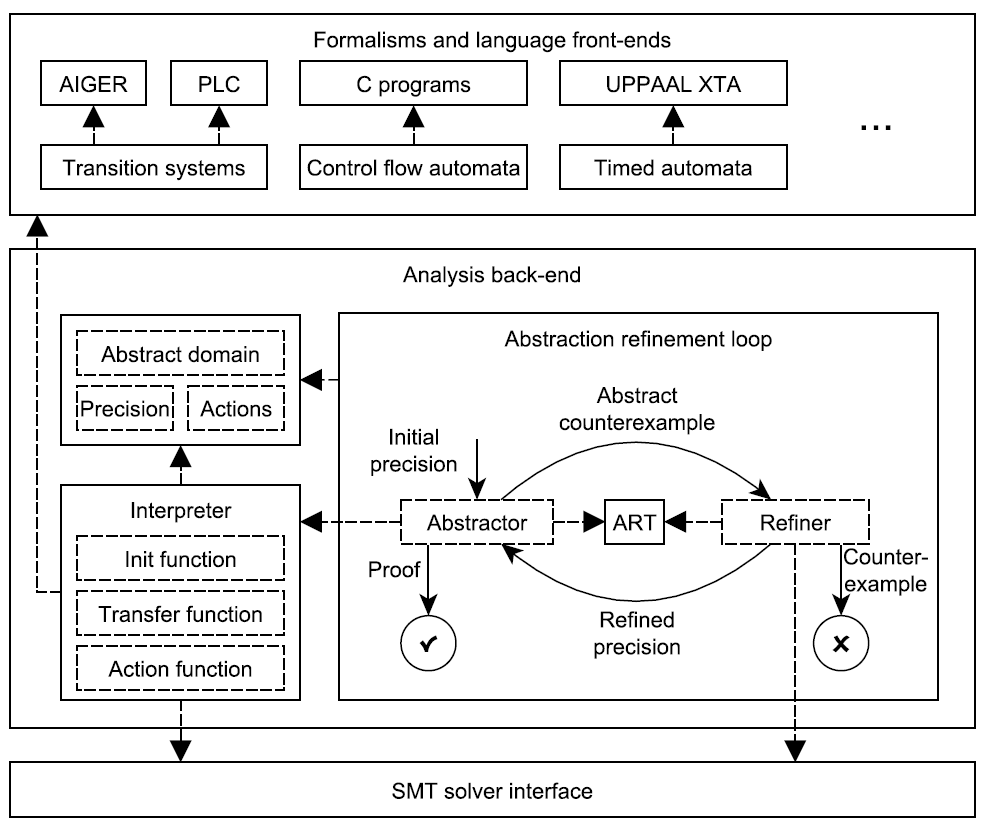
\includegraphics[width=0.9\textwidth, keepaspectratio]{figures/theta.png}
    \caption{A Theta keretrendszer felépítése \cite{Theta}}
    \label{fig:theta}
\end{figure}

A Theta felépítését tekintve három fő részre osztható: a formalizmusok és nyelvi front-endek (\emph{formalisms and language front-ends}), az analízis back-end (\emph{analysis back-end}) és az SMT megoldó interfész (\emph{SMT solver interface}).

A Theta egyik célja, hogy különböző formalizmusokat is támogasson. Az alacsony szintű matematikai reprezentációkhoz (elsőrendű logika kifejezések, gráfalapú leírások) magasabb szintű nyelvi front-endek is tartoznak, amelyek parszerek és interpreterek segítségével képződnek le alacsonyabb szintre. A támogatott formalizmusok jelenleg tranzíciós rendszerek (PLC vagy AIGER nyelvről), control flow automaták (C programnyelvből) és időzített automaták (UPPAAL XTA nyelvből). A moduláris felépítésből adódóan azonban a támogatott nyelvek és formalizmusok tovább bővíthetők, a dolgozat írásakor végéhez közeledik az XSTS és XCFA formalizmusok fejlesztése.

Az analízis back-end három fő részből áll: az absztrakt doménből (\emph{abstract domain}), a formalizmusfüggő interpreterből (\emph{interpreter}) és az absztrakciófinomítási ciklusból (\emph{abstraction refinement loop}).

Az analízis alapja az absztrakt domén, az absztrakt állapotok halmazával (valamint az alsó elemmel és egy állapotokon értelmezett részleges rendezéssel). Egy adott analízis pontosságát (\emph{precision}) a modellből nyilvántartott információk halmaza adja. Továbbá az adott formalizmus meghatározza az akciók halmazát (\emph{actions}).

Az interpreter definiálja az absztrakt állapotokon és akciókon értelmezett működési szemantikát, adott pontossággal. Az absztrakt kezdőállapotokat az inicializáló függvény (\emph{init function}) adja meg, míg egy absztrakt állapotot adott akcióra követő utód állapot az átviteli függvénnyel (\emph{transfer function}) számítható ki. Az akció függvény (\emph{action function}) az elérhető akciókat rendeli egy absztrakt állapothoz.

Az elérhetőség analízist az absztrakciófinomítási ciklus végzi el, melynek központi adatstruktúrája az absztrakt elérhetőségi fa (\emph{ART: abstract reachability tree}), melynek csúcsai absztrakt állapotokkal (amik elérhető állapotok absztrakt felülbecslései), élei pedig akciókkal címkézettek. A \ref{def:ASG}. definícióban bevezetett Adaptive Simulation Graph is egy ART az XTA formalizmushoz. Az ART-t a ciklus két fő eleme módosítja: az absztraháló (\emph{abstractor}) és a finomító (\emph{refiner}).

Az interpreter segítségével a kezdeti pontosság (\emph{initial precision}) és az adott absztrakciós stratégia (algoritmus) alapján az absztraháló előállítja a kezdeti ART-t. Ha az ART-ben nincs ellenpélda, az bizonyítja (\emph{proof}) a modell helyességét (biztonságosságát). Ellenkező esetben (vagyis ha az absztraháló az ART-ben talál absztrakt ellenpéldát) a finomító ellenőrzi az absztrakt ellenpélda elérhetőségét. Amennyiben elérhető, vagyis valódi ellenpélda, a modell hibás (nem biztonságos), egyébként pedig a finomító úgy finomítja az ART absztrakcióját, hogy ezt a valójában nem elérhető ellenpéldát már ne tartalmazza (lásd \ref{modellellenorzes}. fejezet).

Az SMT megoldó interfész egy általános interfész, amely támogatja többek között az inkrementális megoldást is (\aref{smt-megoldok}. fejezetben bemutatott \textsc{Push} és \textsc{Pop} műveletek). Ezt az interfészt használják az analízis komponensek az állapotok részleges rendezéséhez és az átviteli függvényhez, de a finomító is használhatja egy absztrakt ellenpélda elérhetőségének vizsgálatához vagy az absztrakció finomításához, Az interfészt többek között a jelenleg elsődlegesen használt Z3 SMT megoldó implementálja, de könnyen bővíthető további megoldókkal.

\subsection{Megvalósítás}

A Theta Java\footnote{\url{https://www.java.com/}} nyelven írt, nyílt forráskódú\footnote{\url{https://github.com/ftsrg/theta}} szoftver. A fentebb ismertetett modularitás a szoftver megvalósításában is tetten érhető: az elkülöníthető modulok külön alprojektekben (\emph{subproject}) és csomagokban (\emph{package}) találhatók. A \ref{table:theta-packages}. táblázatban láthatók rendszerezve a Theta alprojektjei.

Az analízis formalizmusfüggetlen, közös komponenseit az \textsf{analysis} alprojekt tartalmazza. Itt találhatók az analízis algoritmusok és komponenseik, mint pl. absztrakt domén, absztrakt elérhetőségi gráf, finomítási stratégiák, pontosságok stb.

A \textsf{common} alprojekt tartalmazza az általános fejlesztéshez kapcsolódó osztályokat, többek között a logoláshoz és megjelenítéshez kapcsolódóan. A formalizmusok leírásához szükséges közös komponensek a \textsf{core} alprojektben találhatók. Itt találhatók a típusok, konstansok, változók, kifejezések, modellek és utasítások.

Az általános SMT megoldó interfészt a \textsf{solver}, a Z3 implementációját pedig a \textsf{solver-z3} alprojekt tartalmazza.

\begin{table}
\centering
\begin{tabular}{ |c||c|c|c|c|c| } 
 \hline
  & Közös & CFA & STS & XTA & XSTS \\ 
 \hline
 \hline
 Eszközök & & \textsf{cfa-cli} & \textsf{sts-cli} & \textsf{xta-cli} & \textsf{xsts-cli} \\ 
 \hline
 Analízis & \textsf{analysis} & \textsf{cfa-analysis} & \textsf{sts-analysis} & \textsf{xta-analysis} & \textsf{xsts-analysis} \\ 
 \hline
 Formalizmusok & \textsf{core}, \textsf{common} & \textsf{cfa} & \textsf{sts} & \textsf{xta} & \textsf{xsts} \\ 
 \hline
 SMT megoldók & \textsf{solver}, \textsf{solver-z3} & & & & \\
 \hline
\end{tabular}
\caption{A Theta keretrendszer alprojektjei}
\label{table:theta-packages}
\end{table}

A Theta által támogatott konkrét formalizmusok külön projektekben találhatók. Jelenleg a következő formalizmusok támogatottak: control flow automaták (\textsf{cfa}), (kiterjesztett) szimbolikus tranzíciós rendszerek (\textsf{sts} / \textsf{xsts}) és időzített automaták (\textsf{xta}).

A formalizmusspecifikus analízis modulok külön alprojektekben találhatók, melyek neve a formalizmus nevéből és az \textsf{-analysis} végződésből áll (\textsf{cfa-analysis}, \textsf{sts-analysis}, \textsf{xta-analysis}, \textsf{xsts-analysis}).

A formalizmusspecifikus eszközök egyszerű parancssoros programok (\emph{command line interface}), melyek futtatható jar fájllá fordíthatók. Feladatuk többnyire csak az inputok beolvasása, majd a megfelelő algoritmus példányosítása és meghívása. Ezek az eszközök is külön alprojektekben találhatók, melyek neve a formalizmus nevéből és a \textsf{-cli} végződésből áll (\textsf{cfa-cli}, \textsf{sts-cli}, \textsf{xta-cli}, \textsf{xsts-cli}).

Munkám során az XTA-hoz kapcsolódó részeket egészítettem ki, a modularitást szem előtt tartva amennyire csak lehetséges, külön alprojektben és csomagban.
%own chapters...
% TeXstudio spellcheck 2020-12-10 16:34

\chapter{Valós idejű tesztek generálása vezérlési helyekhez}\label{main-elmelet}

Ebben a fejezetben formalizálom a munkám során használt fogalmakat (\ref{teszt-tesztkeszlet}. fejezet), majd meghatározom a generálandó tesztkészlettel kapcsolatos elvárásokat (\ref{kovetelmenyek}. fejezet). Bemutatom a tesztesetek útvonalát (\ref{teszt-utvonal}. fejezet) és időzítését (\ref{teszt-idozites}. fejezet) generáló algoritmusokat, majd utóbbit visszavezetem egy SMT problémára (\ref{teszt-smt}. fejezet). Végül belátom, hogy a bemutatott algoritmusokkal generált tesztkészlet valóban teljesíti \aref{kovetelmenyek}. fejezetben megfogalmazott elvárásokat (\ref{kovetelmenyek-telj}. fejezet), majd leírom a szükséges kimeneti formátumokat (\ref{kimenet}. fejezet).

A cél a bemenetként kapott időzített automata vezérlési helyeinek lefedése valós idejű (konkrét időzítésű) tesztekkel. A bemenetünk nemcsak egy, hanem tetszőleges (véges) számú időzített automata hálózata is lehet. Ehhez először is definiálnunk kell, hogy milyen tesztkészletet szeretnénk generálni (vagyis hogy milyen követelményeket támasztunk a tesztkészlettel szemben).

Ezt követően fel kell dolgoznunk az időzített automatát. Egy véges, absztrakt adatszerkezetre (ASG) képezzük le, amelyet bejárva absztrakt teszteseteket tudunk generálni. Egy absztrakt tesztesethez konkrét időzítést kell generálni (vagyis konkretizálni kell a tesztet), hogy valós idejű tesztet kapjunk belőle.

\section{Teszt, tesztkészlet} \label{teszt-tesztkeszlet}
Egy időzített automatán értelmezett valós idejű teszt az automata egy konkrét lefutása (vezérlési helyek és élek alternáló időzített sorozata).

Jelölje egy $\mathcal{A}$ időzített automata vezérlési helyeinek halmazát $L(\mathcal{A})$, kezdő vezérlési helyét $l_0(\mathcal{A})$, éleinek halmazát $T(\mathcal{A})$, invariánsainak halmazát $I(\mathcal{A})$.

\begin{definition}[Valós idejű teszt]
\label{ValósIdejűTeszt}
Egy $\mathcal{A}$ időzített automata $n \in \mathbb{N}^+$ hosszúságú $\mathcal{T}$ \emph{valós idejű tesztje} formálisan $\langle \mathcal{A}, Loc, Act, \hat{t} \rangle$, ahol
\begin{itemize}
    \item $\mathcal{A}$ az időzített automata, amin az időzített teszt fut,
    \item $Loc$ az $\mathcal{A}$ automata vezérlési helyeinek $n$ hosszú sorozata, vagyis $|Loc| = n$ és $Loc_i \in L(\mathcal{A})$, ha $1 \leq i \leq n$,
    \item $Act$ az $\mathcal{A}$ automata éleinek $n-1$ hosszú sorozata, vagyis $|Act| = n-1$ és $Act_j \in T(\mathcal{A})$, ha $1 \leq j \leq n-1$,
    \item $\hat{t}$ az időzítések $n$ hosszú sorozata, vagyis $|\hat{t}| = n$ és $\hat{t}_k \in \mathbb{R}_0^+$, ha $1 \leq k \leq n$, amely minden $Loc_k$ vezérlési helyre megadja, hogy a $k.$ lépésben $\hat{t}_k$ időt tölt el ott az automata.
\end{itemize}
\end{definition}

Egy $\automaton$ automatán értelmezett $\test$ valós idejű teszt $i.$ lépése szemantikáját tekintve három lépésből áll, ahol $1 \leq i \leq |\test|$:
\begin{enumerate}
    \item tüzel az automata $Act_{i-1}$ éle, ha $i > 1$,
    \item az automata $\hat{t}_{i}$ ideig várakozik a $Loc_i$ vezérlési helyen,
    \item az óraváltozók a $Loc_i$-beli értékükre váltanak, vagyis a $Loc_i$-beli értékek már a $\hat{t}_{i}$ időnyi várakozás utáni értékekre vonatkozik.
\end{enumerate}

Jelölje egy $\mathcal{T}$ valós idejű teszt esetén $A(\mathcal{T})$ azt az időzített automatát, amelyen a teszt fut (vagyis $A(\langle \mathcal{A}, Loc, Act, \hat{t} \rangle) = \mathcal{A}$), $Loc(\mathcal{T})$ a teszt vezérlési helyeinek sorozatát, $Act(\mathcal{T})$ a teszt éleinek sorozatát, $\hat{t}(\mathcal{T})$ a teszt időzítéseinek sorozatát, $|\mathcal{T}| = |Loc(\mathcal{T})|$ a teszt hosszát, $Loc_s(\mathcal{T}) = \bigcup\limits_{i = 1}^{|Loc(\mathcal{T})|} \{ Loc(\mathcal{T})_i \}$ pedig a teszt által lefedett vezérlési helyek halmazát.

\begin{definition}[Valós idejű teszt valódisága]
\label{ValódiTeszt}
Egy $\mathcal{T}$ valós idejű teszt \emph{valódi}, ha az $A(\mathcal{T})$ időzített automatának valóban van olyan lefutása, amit a teszt leír, vagyis 
\begin{itemize}
    \item $Loc(\mathcal{T})_1 = l_0(A(\mathcal{T}))$, vagyis a $\mathcal{T}$ teszt első vezérlési helye az $A(\mathcal{T})$ automata kezdő vezérlési helye,
    \item minden $Loc(\mathcal{T})_i$ vezérlési helyen $\hat{t}(\mathcal{T})_i$ ideig történő várakozást lehetővé teszik az $A(\mathcal{T})$ automata $I(A(\mathcal{T}))$ invariánsai (vagyis az $A(\mathcal{T})$ időzített automatának van $\langle Loc(\mathcal{T})_i, u \rangle \rightarrow \langle Loc(\mathcal{T})_i, u + \hat{t}(\mathcal{T})_i \rangle$ állapotátmenete, ahol $u$ jelöli az óraváltozók állását, amikor a teszt az $i$. lépésben a $Loc(\mathcal{T})_i$ vezérlési helyre lép), ahol $1 \leq i \leq |\test|$,
    \item minden $Act(\mathcal{T})_i$ élhez van olyan éle az $A(\mathcal{T})$ automatának, amely $Loc(\mathcal{T})_i$ vezérlési helyből $Loc(\mathcal{T})_{i+1}$ vezérlési helybe vezet, és $Loc(\mathcal{T})_i$ vezérlési helyen $\hat{t}(\mathcal{T})_i$ ideig való várakozás után tüzelhető (vagyis az $A(\mathcal{T})$ időzített automatának van $\langle Loc(\mathcal{T})_i, u \rangle \rightarrow \langle Loc(\mathcal{T})_{i+1}, u' \rangle$ állapotátmenete, ahol $u$ jelöli az óraváltozók állását, amikor a teszt az $i$. lépésben $\hat{t}(\mathcal{T})_i$ időt eltöltött a $Loc(\mathcal{T})_i$ vezérlési helyen), ahol $1 \leq i \leq |\test| - 1$.
\end{itemize}
\end{definition}

\begin{definition}[Valós idejű tesztkészlet]
\label{Tesztkészlet}
Egy $\mathcal{A}$ időzített automata $n$ elemű $\mathfrak{T}$ \emph{valós idejű tesztkészlete} valós idejű tesztek $n \in \mathbb{N}^+$ elemű halmaza ($|\mathfrak{T}| = n$), amelynek minden $\mathfrak{T}_i$ tesztjére $A(\mathfrak{T}_i) = \mathcal{A}$, ahol $1 \leq i \leq n$.
\end{definition}

A valós idejű tesztek tulajdonságait kiterjeszthetjük a valós idejű tesztkészletekre is. Jelöljön $\mathfrak{T}$ egy valós idejű tesztkészletet.
\begin{itemize}
    \item $A(\mathfrak{T}) = A(\mathfrak{T}_i)$, ahol $1 \leq i \leq |\mathfrak{T}|$
    \item $Loc_s(\mathfrak{T}) = \bigcup\limits_{i = 1}^{|\mathfrak{T}|} Loc_s(\mathfrak{T}_i)$ a $\mathfrak{T}$ által lefedett vezérlési helyek halmaza
    \item $\mathfrak{T}$ \emph{valódi}, ha minden $\mathfrak{T}_i$ tesztje valódi, ahol $1 \leq i \leq |\mathfrak{T}|$
\end{itemize}

\subsection{Kiterjesztés időzített automaták hálózatára}

A fent bevezetett fogalmak nemcsak egyetlen időzített automatára értelmezhetők, hanem kiterjeszthetők időzített automaták véges hálózatára (halmazára) is. Jelölje $\hat{\mathcal{A}}$ időzített automaták $n \in \mathbb{N}^+$ elemű hálózatát ($|\hat{\mathcal{A}}| = n$), $\hat{\mathcal{A}}_i$ pedig a hálózat egy automatáját ($1 \leq i \leq n$). Jelölje továbbá $L(\automatanetwork)$ az $\automatanetwork$-beli automaták vezérlési helyeinek halmazát, azaz $L(\automatanetwork) = \bigcup\limits_{i = 1}^{|\automatanetwork|} L(\automatanetwork_i)$; $T(\automatanetwork)$ pedig az $\automatanetwork$-beli automaták éleinek halmazát, azaz $T(\automatanetwork) = \bigcup\limits_{i = 1}^{|\automatanetwork|} T(\automatanetwork_i)$. Jelölje $\varepsilon$ az üres élt (amikor az automata egyik éle sem tüzel), ekkor $T_\varepsilon(\automatanetwork) = T(\automatanetwork) \cup \{ \varepsilon \}$

\begin{definition}[Valós idejű teszt kiterjesztése]
\label{ValósIdejűTesztKiterjesztés}
Időzített automaták $\hat{\mathcal{A}}$ hálózatának $n \in \mathbb{N}^+$ hosszúságú $\hat{\mathcal{T}}$ valós idejű tesztje formálisan $\langle \hat{\mathcal{A}}, \hat{L}oc, \hat{A}ct, \hat{t} \rangle$, ahol

\begin{itemize}
    \item $\hat{\mathcal{A}}$ az időzítettautomata-hálózat, amin az időzített teszt fut,
    \item $\hat{L}oc: \automatanetwork \rightarrow L(\automatanetwork)^n$  az automatahálózat minden $\automatanetwork_i$ automatájához egy $n$ elemű $\hat{L}oc(\automatanetwork_i)$ vezérlésihely-vektort rendel, amelynek $j.$ eleme megadja az $\automatanetwork_i$ automata aktív vezérlési helyét a teszt $j.$ lépésében, vagyis $\hat{L}oc(\automatanetwork_i)_j \in L(\automatanetwork_i)$, ahol $1 \leq i \leq |\automatanetwork|$ és $1 \leq j \leq n$,
    %\item $\hat{L}oc$ az $\hat{\mathcal{A}}$ automatahálózat $n$ hosszú vezrélésihely-vektor sorozata, amelynek minden $\hat{L}oc_i$ eleme egy $|\hat{\mathcal{A}}|$ hosszú vektor, ahol $1 \leq i \leq n$. $\hat{L}oc_i_j$ az $\hat{\mathcal{A}}_j$ automata aktív vezérlési helye a teszt $i.$ lépésében, vagyis $\hat{L}oc_i_j \in L(\hat{\mathcal{A}}_j)$, ahol $1 \leq j \leq |\hat{\mathcal{A}}|$,
    
    %\item $\hat{A}ct$ az $\hat{\mathcal{A}}$ automatahálózat $n - 1$ hosszú élvektor sorozata, és minden $T_i$ él valamely $\hat{\mathcal{A}}_j$ automata éle, vagyis minden $i$-re $T_i \in T(\hat{\mathcal{A}}_j)$, ahol $1 \leq i \leq n - 1$ és $1 \leq j \leq |\hat{\mathcal{A}}|$,
    
    \item $\hat{A}ct: \automatanetwork \rightarrow T_\varepsilon(\automatanetwork)^{n-1}$  az automatahálózat minden $\automatanetwork_i$ automatájához egy $n-1$ elemű $\hat{A}ct(\automatanetwork_i)$ élvektort rendel (amelyben $\varepsilon$ jelöli az üres élt), amelynek $j.$ eleme megadja az $\automatanetwork_i$ automata által tüzelt élt a teszt $j.$ lépésében, vagyis $\hat{A}ct(\automatanetwork_i)_j \in T(\automatanetwork_i) \cup \{ \varepsilon \}$, ahol $1 \leq i \leq |\automatanetwork|$ és $1 \leq j \leq n$,
    
    %\item $\hat{A}ct$ az $\hat{\mathcal{A}}$ automatahálózat éleinek $n - 1$ hosszú sorozata, és minden $T_i$ él valamely $\hat{\mathcal{A}}_j$ automata éle, vagyis minden $i$-re $T_i \in T(\hat{\mathcal{A}}_j)$, ahol $1 \leq i \leq n - 1$ és $1 \leq j \leq |\hat{\mathcal{A}}|$,
    \item $\hat{t}$ az időzítések $n$ hosszú sorozata, vagyis $|\hat{t}| = n$ és $\hat{t}_i \in \mathbb{R}_0^+$, ha $1 \leq i \leq n$, amely megadja, hogy az $i.$ lépésben $\hat{t}_i$ időt tölt minden $\automatanetwork_j$ automata a $\hat{L}oc(\automatanetwork_j)_i$ vezérlési helyen, ahol $1 \leq j \leq |\automatanetwork|$.
\end{itemize}
\end{definition}

Egy $\automatanetwork$ automatahálózaton értelmezett $\networktest$ teszteset $i.$ lépésének szemantikája a $\test$-nél bemutatotthoz hasonlóan, ahol $1 \leq i \leq |\networktest|$:
\begin{enumerate}
    \item tüzel az automatahálózat minden $\automaton \in \automatanetwork$ automatájának $\hat{A}ct(\automaton)_{i - 1}$ éle, ha $i > 1$ és $\hat{A}ct(\automaton)_{i - 1} \neq \varepsilon$,
    \item az automatahálózat minden $\automaton \in \automatanetwork$ automatája $\hat{t}_i$ ideig várakozik a $\hat{L}oc(\automaton)_{i}$ vezérlési helyen,
    \item az automatahálózat minden $\automaton \in \automatanetwork$ automatájának óraváltozói $\hat{L}oc(\automaton)_{i}$-beli értékükre váltanak, vagyis az óraváltozók $\hat{L}oc(\automaton)_{i}$-beli értéke már a $\hat{t}_i$ időnyi várakozás utáni értékekre vonatkozik.
\end{enumerate}

Jelölje egy $\networktest$ valós idejű teszt esetén $\hat{A}(\networktest)$ azt az időzítettautomata-hálózatot, amelyen a teszt fut (vagyis $\hat{A}(\langle \automatanetwork, \hat{L}oc, \hat{A}ct, \hat{t} \rangle) = \automatanetwork$), $\hat{L}oc(\networktest)$ a teszt vezérlésihelyvektor-hozzárendelését, $\hat{A}ct(\networktest)$ a teszt élvektor-hozzárendelését, $\hat{t}(\networktest)$ a teszt időzítéseinek sorozatát, $|\networktest| = |\hat{L}oc(\hat{A}(\networktest)_i)|$ a teszt hosszát (ahol $1 \leq i \leq |\hat{A}(\networktest)|$), $\hat{L}oc_s(\networktest) = \bigcup\limits_{i = 1}^{|\hat{A}(\networktest)|} \hat{L}oc(\hat{A}(\networktest)_i)$ pedig a teszt által lefedett vezérlési helyek halmazát.

Megjegyzendő, hogy míg egyetlen $\automaton$ időzített automatán futó $\test$ teszt esetén a teszt vezérlési helyek és élek alternáló sorozata, időzített automaták $\automatanetwork$ hálózatán futó $\networktest$ teszt esetén egy adott lépésben a rendszer aktív vezérlési helyeit az összes automata aktív vezérlési helye együttesen határozza meg.

Hasonlóan kiemelendő, hogy utóbbi esetben a teszt egy lépésében több $\automatanetwork_i$ automatának ($1 \leq i \leq |\hat{A}(\networktest)|$) is tüzelhet éle (vagyis egy adott $j.$ lépésben ($1 \leq j \leq |\networktest| - 1$) $k$ számú $\automatanetwork_i$ automatára is fennállhat, hogy $\hat{A}ct(\automatanetwork_i)_j \neq \varepsilon$, ahol $1 \leq k \leq |\hat{A}(\networktest)|$). Ez teszi lehetővé, hogy egy automatahálózat automatái élekkel szinkronizálják működésüket, vagyis automaták egy-egy éle \emph{egyszerre} tüzeljen.

Egy $\networktest$ teszteset hossza (időben) a lépésekben eltöltött várakozási idők összege, vagyis $time(\networktest) = \sum\limits_{i = 1}^{|\networktest|} \hat{t}_i$.

\begin{definition}[Valós idejű teszt valódiságának kiterjesztése]
\label{ValódiTesztKiterjesztés}
Egy $\networktest$ valós idejű teszt \emph{valódi}, ha az $\hat{A}(\networktest)$ időzítettautomata-hálózatnak valóban van olyan lefutása, amit a teszt leír, vagyis 
\begin{itemize}
    \item $\hat{L}oc(\hat{A}(\networktest)_i)_1 = l_0(\hat{A}(\networktest)_i)$, vagyis az $\hat{A}(\networktest)$ időzítettautomata-hálózat minden $\hat{A}(\networktest)_i$ automatájának vezérlésihely-vektorának első eleme az automata kezdő vezérlési helye, ahol $1 \leq i \leq |\hat{A}(\networktest)|$,
    %\item OFF $\hat{L}(\hat{\mathcal{T}})_1_i = l_0(\hat{A}(\hat{\mathcal{T}})_i)$, vagyis a $\hat{\mathcal{T}}$ teszt első vezérlésihely-vektora az $\hat{A}(\hat{\mathcal{T}})$ automatahálózat minden $\hat{A}(\hat{\mathcal{T}})_i$ automatájának a kezdő vezérlési helyét tartalmazza, ahol $1 \leq i \leq |\hat{A}(\hat{\mathcal{T}})|$,
    \item minden $\hat{A}(\networktest)_i$ automata minden $\hat{L}oc(\hat{A}(\networktest)_i)_j$ vezérlési helyén lehetővé teszik az automata $I(\hat{A}(\networktest)_i)$ invariánsai a $\hat{t}_j$ ideig történő várakozást (vagyis minden $\hat{A}(\networktest)_i$ időzített automatának van $\langle \hat{L}oc(\hat{A}(\networktest)_i)_j, u \rangle \rightarrow \langle \hat{L}oc(\hat{A}(\networktest)_i)_j, u + \hat{t}_j \rangle$ állapotátmenete, ahol $u$ jelöli az óraváltozók állását, amikor a teszt $j.$ lépésben az automata a $\hat{L}oc(\hat{A}(\networktest)_i)_j$ vezérlési helyre lép), ahol $1 \leq i \leq |\hat{A}(\networktest)|$ és $1 \leq j \leq |\networktest|$,
    %\item minden $L(\mathcal{T})_i$ vezérlési helyen $t(\mathcal{T})_i$ ideig történő várakozást lehetővé teszik az $A(\mathcal{T})$ automata $I(A(\mathcal{T}))$ invariánsai (vagyis az $A(\mathcal{T})$ időzített automatának van $\langle L(\mathcal{T})_i, u \rangle \rightarrow \langle L(\mathcal{T})_i, u + t(\mathcal{T})_i \rangle$ állapotátmenete, ahol $u$ jelöli az óraváltozók állását, amikor a teszt az $i$. lépésben az $L(\mathcal{T})_i$ vezérlési helyre lép),
    \item minden $\hat{A}ct(\hat{A}(\networktest)_i)_j$ élhez van olyan éle az $\hat{A}(\networktest)_i$ automatának, amely a $\hat{L}oc(\hat{A}(\networktest)_i)_j$ vezérlési helyből a $\hat{L}oc(\hat{A}(\networktest)_i)_{j+1}$ vezérlési helybe vezet, és $\hat{L}oc(\hat{A}(\networktest)_i)_j$ vezérlési helyen $\hat{t}_j$ ideig való várakozás után tüzelhető (vagyis minden $\hat{A}(\networktest)_i$ időzített automatának van $\langle \hat{L}oc(\hat{A}(\networktest)_i)_j, u \rangle \rightarrow \langle \hat{L}oc(\hat{A}(\networktest)_i)_{j+1}, u' \rangle$ állapotátmenete, ahol $u$ jelöli az óraváltozók állását, amikor a teszt $j.$ lépésében az $\hat{A}(\networktest)_i$ automata $\hat{t}_j$ időt eltöltött a $\hat{L}oc(\hat{A}(\networktest)_i)_j$ vezérlési helyen), ahol $1 \leq i \leq |\hat{A}(\networktest)|$ és $1 \leq j \leq |\networktest| - 1$.
    %\item minden $T(\mathcal{T})_i$ élhez van olyan éle az $A(\mathcal{T})$ automatának, amely $L(\mathcal{T})_i$ vezérlési helyből $L(\mathcal{T})_{i+1}$ vezérlési helybe vezet, és $L(\mathcal{T})_i$ vezérlési helyen $t(\mathcal{T})_i$ ideig való várakozás után tüzelhető (vagyis az $A(\mathcal{T})$ időzített automatának van $\langle L(\mathcal{T})_i, u \rangle \rightarrow \langle L(\mathcal{T})_{i+1}, u' \rangle$ állapotátmene, ahol $u$ jelöli az óraváltozók állását, amikor a teszt az $i$. lépésben $t(\mathcal{T})_i$ időt eltöltött $L(\mathcal{T})_i$ vezérlési helyen).
\end{itemize}
\end{definition}

\begin{definition}[Valós idejű tesztkészlet kiterjesztése]
\label{TesztkészletKiterjesztés}
Egy $\automatanetwork$ időzítettautomata-hálózat $n$ elemű $\networktestset$ \emph{valós idejű tesztkészlete} valós idejű tesztek $n \in \mathbb{N}^+$ elemű halmaza ($|\networktestset| = n$), amelynek minden $\networktestset_i$ tesztjére $\hat{A}(\networktestset_i) = \automatanetwork$, ahol $1 \leq i \leq n$.
\end{definition}

A valós idejű tesztek tulajdonságait ezúttal is kiterjeszthetjük a valós idejű tesztkészletekre. Jelöljön $\networktestset$ egy valós idejű tesztkészletet.
\begin{itemize}
    \item $\hat{A}(\networktestset) = \hat{A}(\networktestset_i)$, ahol $1 \leq i \leq |\networktestset|$
    \item $\hat{L}oc_s(\networktestset) = \bigcup\limits_{i = 1}^{|\networktestset|} \hat{L}oc_s(\networktestset_i)$ a $\networktestset$ által lefedett vezérlési helyek halmaza
    \item $\networktestset$ \emph{valódi}, ha minden $\networktestset_i$ tesztje valódi, ahol $1 \leq i \leq |\networktestset|$
\end{itemize}

\section{A tesztkészlet elvárt tulajdonságai} \label{kovetelmenyek}

Tekintsük a tesztgenerálási folyamatot egy $TG: \automatanetwork \rightarrow \networktestset$ hozzárendelésnek, ahol $\automatanetwork$ a bemenetként kapott időzítettautomata-hálózat, $\networktestset$ pedig az $\automatanetwork$ hálózat kimenetként generált valós idejű tesztkészlete.

A $\networktestset$ valós idejű tesztkészlettel szemben több elvárást is támasztunk:

\begin{enumerate}
    \item \label{kov:valodi} $\networktestset$ legyen valódi, vagyis a tesztek valóban $\automatanetwork$ lefutásai legyenek,
    \item \label{kov:fedes} $\networktestset$ fedje le $\automatanetwork$ összes \emph{elérhető} vezérlési helyét, vagyis ha minden vezérlési hely elérhető, akkor $\hat{L}oc_s(\networktestset) = L(\automatanetwork)$,
    \item \label{kov:tesztekhossza} $\networktestset$ tesztjei minél rövidebbek legyenek, vagyis $\min |\networktestset_i|$, ahol $1 \leq i \leq |\networktestset|$,
    \item \label{kov:tesztekszama} $\networktestset$ minél kevesebb tesztből álljon, vagyis $\min |\networktestset|$,
    \item \label{kov:tesztekideje} $\networktestset$ tesztjei minél rövidebb ideig fussanak, vagyis $\min time(\networktestset_i)$, ahol $1 \leq i \leq |\networktestset|$,
    \item \label{kov:prefixteszt} (\ref{kov:tesztekszama}. követekzménye) $\networktestset$ egyik tesztje se legyen prefixe egy másiknak, vagyis $\nexists \networktestset_i, \networktestset_j$, hogy $\forall k, l: \hat{L}oc(\networktestset_i)(\hat{A}(\networktestset)_k)_l = \hat{L}oc(\networktestset_j)(\hat{A}(\networktestset)_k)_l$, ahol $1 \leq i \neq j \leq |\networktestset|$, $1 \leq k \leq |\hat{A}(\networktestset)|$ és $1 \leq l \leq |\networktestset_i|$.
\end{enumerate}

\section{A tesztek útvonala} \label{teszt-utvonal}

Az $\automatanetwork$ automatahálózat helyesen címkézett ASG-jének bejárásával keressük meg azokat az absztrakt lefutásokat, amelyek konkrét időzítés után $\networktestset$ tesztjei lesznek.

Jelölje $G = \langle V, E, v_0, M_v, M_e, \rhd, \psi_Z, \psi_W \rangle$ az $\automatanetwork$ hálózat helyesen címkézett ASG-jét. Jelölje $V(G)$ $V$-t, $E(G)$ $E$-t, $v_0(G)$ $v_0$-t stb., $\hat{A}(G)$ pedig azt az időzítettautomata-hálózatot, amelyet $G$ reprezentál.

Legyen $v \in V$ a $G$ ASG egy csúcsa. Jelölje $\textsc{Children}(v)$ azoknak a $V$-beli csúcsoknak a halmazát, amelyekbe vezet él $v$-ből, $\textsc{Ancestor}(v)$ azt a $V$-beli csúcsot, amelyből vezet él $v$-be, $\textsc{InEdge}(v)$ pedig azt az $E$-beli élt, amely $v$-be vezet.

Jelölje továbbá $\hat{L}oc(v): \automatanetwork \rightarrow L(\automatanetwork)$ azt a hozzárendelést, amely az $\automatanetwork$ hálózat minden automatájára megadja, hogy a $v$ csúcs által reprezentált absztrakt állapotban az automata melyik vezérlési helye aktív.

Legyen $e \in E$ a $G$ ASG egy éle. Jelölje $\hat{A}ct(e): \automatanetwork \rightarrow T_\varepsilon(\automatanetwork)$ azt a hozzárendelést, amely az $\automatanetwork$ hálózat minden automatájára megadja, hogy az $e$ él által reprezentált absztrakt élen az automata melyik éle tüzel ($\varepsilon$ jelöli azt, hogy egyik sem).

$G$ egy $v \in V$ csúcsa egy olyan absztrakt állapotot ír le, amelyben az $\automatanetwork$ hálózat $M_v(v)$ vezérlési helyei aktívak, egy $e \in E$ éle pedig egy olyan absztrakt átmenetet, amely során az $\automatanetwork$ hálózat $M_e(e)$ élei tüzelnek. $G$-beli úton egy $(V, E)$-beli utat értünk, vagyis $V$-beli csúcsok és $E$-beli élek alternáló sorozatát.

Egy $G$-beli út egy absztrakt (konkrét időzítés nélküli) tesztesetet ír le, vagyis meghatározza a $\networktest$ teszteset $\hat{L}oc(\networktest)$ és $\hat{A}ct(\networktest)$ hozzárendeléseit, míg a konkrét $\hat{t}(\networktest)$ időzítést majd csak a konkretizálás fogja meghatározni.

Egy $(K \mapsto V)$ kulcs-érték párokat tartalmazó $M$ \emph{map} (hozzárendelés) esetén $\textsc{Keys}(M)$ a $K$ kulcsok halmazát, míg $\textsc{Values}(M)$ a $V$ értékek halmazát jelöli. $M(K) = V$, ha $(K \mapsto V) \in M$.

Az üres \emph{listát}  $[\ ]$ jelöli, egy $X$ lista esetén az $a$ elem beszúrását a lista elejére az $X \gets [a, X]$, a lista végére pedig az $X \gets [X, a]$ művelet jelöli.

A tesztkészlet-generálás \textsc{GenerateTests} algoritmusát az \ref{GenerateTests}. algoritmus írja le, amely felhasználja a \ref{GenerateTest}. algoritmusban leírt \textsc{GenerateTest} segédeljárást, amely egy adott ASG-csúcshoz generál tesztet.

A $\networktestset$-vel szemben támasztott \ref{kov:fedes}. követelmény miatt addig kell új teszteseteket (utakat) keresnünk $G$-ben, amíg minden $L(\automatanetwork)$-beli vezérlési helyet lefed már legalább egy teszteset vagy a teljes $G$ ASG-t bejártuk (amennyiben $G$ teljes bejárása után sem találtunk egy vezérlési helyhez azt fedő utat, a vezérlési hely nem elérhető, vagyis a lefedése nélkül is teljesítjük \aref{kov:fedes}. követelményt). A $locTests: L(\automatanetwork) \rightarrow \networktestset$ hozzárendelés $\automatanetwork$ minden vezérlési helyére megad egy azt fedő $\networktestset_i$ tesztesetet.

$G$-t szélességi bejárással járjuk be (amíg szükséges), hogy a kapott tesztesetek a lehető legrövidebbek legyenek (\ref{kov:tesztekhossza}. követelmény). A $nodesToProcess$ halmaz tartalmazza az éppen feldolgozandó csúcsokat, $nextNodes$ halmaz pedig a következő lépésben feldolgozandókat ($nextNodes$-ba kerülnek a $nodesToProcess$-ből elérhető csúcsok). $G$ teljes bejárását az jelzi, ha egy iteráció után $nodesToProcess = \emptyset$.

Egy $node$ csúcs feldolgozása során először egy időzítetlen $\networktest$ tesztet generálunk hozzá a \textsc{GenerateTest} eljárás segítségével, majd a $\networktest$ által fedett $\hat{L}oc_s(\networktest)$ vezérlési helyekre frissítjük a $locTests$-et, hogy minden $l \in \hat{L}oc_s(\networktest)$-re $locTests(l) = \networktest$ legyen. Ezt a frissítést azokra a vezérlési helyekre is elvégezzük, amelyeket már lefedett egy korábban megtalált teszt, hogy az eredményül kapott tesztkészlet megfeleljen a \ref{kov:tesztekszama}. és \ref{kov:prefixteszt}. követelménynek.

Minden tesztgenerálás után leellenőrizzük, hogy lefedtünk-e már minden vezérlési helyet, és amennyiben igen, kilépünk a ciklusból. Amennyiben az ASG végére értünk ($nodesToProcess = \emptyset$), szintén leáll az algoritmus. Végül a $locTests$ mapben értékként tárolt időzítetlen tesztek időzítését a \textsc{CalculateDelays} eljárással kiszámítjuk, majd az így kapott valós idejű tesztek $realTimeTests$ halmazát adjuk eredményül, amely egy az elvárásokat kielégítő tesztkészlet.

Az ASG felderítése során azért időzítés nélküli teszteseteket generálunk, mert a korábban megtalált teszteseteket a későbbi generálások során még eldobhatjuk, az időzítést leíró SMT probléma megoldása pedig számításigényes feladat. Így viszont biztosan csak az eredmény tesztkészletben ténylegesen szereplő tesztesetek időzítését számítjuk ki.

\begin{algorithm}[t]
\DontPrintSemicolon
\caption{{\sc GenerateTests} Valós idejű tesztkészlet generálása időzített automaták hálózatához} \label{GenerateTests}
\KwIn{Időzített automaták $\automatanetwork$ hálózatát leíró $G = \langle V, E, v_0, M_v, M_e, \rhd, \psi_Z, \psi_W \rangle$ ASG ($\hat{A}(G) = \automatanetwork$)}
\KwOut{Az $\automatanetwork$ hálózat $\networktestset$ valós idejű tesztkészlete ($\hat{A}(\networktestset) = \automatanetwork$)}
\SetKwProg{GenerateTests}{GenerateTests}{}{}

\GenerateTests{$(G)$}{
 $locTests \gets \emptyset$\;
 $nodesToProcess \gets \{ v_0(G) \}$\;
 $nextNodes \gets \emptyset$\;
 \While{$|locTests| < |L(\automatanetwork)| \land nodesToProcess \neq \emptyset$}{
  \ForEach{$node \in nodesToProcess$} {
   $\networktest \gets \textsc{GenerateTest}(G, node)$\;
   \ForEach{$loc \in \hat{L}oc_s(\networktest)$}{ \label{GenerateTests:locTestsForEach}
    $locTests \gets locTests \setminus \{ (loc \mapsto locTests(loc)) \} \cup \{ (loc \mapsto \networktest) \}$\;
    \tcp*{$loc$ leképezésének beállítása $\networktest$-ra}
   }
   \ForEach{$child \in \textsc{Children}(node)$}{
    $nextNodes \gets nextNodes \cup \{ child \}$\;
   }
   \If{$|locTests| = |L(\automatanetwork)|$}{
    \textbf{break}\;
   }
  }
  $nodesToProcess \gets nextNodes$\;
  $nextNodes \gets \emptyset$\;
 }
 $realTimeTests \gets \emptyset$\;
 \ForEach{$\langle \automatanetwork, \hat{L}oc, \hat{A}ct, [\ ] \rangle \in \textsc{Values}(locTests)$}{
  $\hat{t} \gets \textsc{CalculateDelays}(\automatanetwork, \hat{L}oc, \hat{A}ct)$\;
  $realTimeTests \gets realTimeTests \cup \{ \langle \automatanetwork, \hat{L}oc, \hat{A}ct, \hat{t} \rangle \}$
 }
\Return{$realTimeTests$}\;
}
\end{algorithm}

\begin{algorithm}[t]
\DontPrintSemicolon
\caption{{\sc GenerateTest} Időzítés nélküli teszt generálása adott ASG-csúcshoz} \label{GenerateTest}
\KwIn{Időzített automaták $\automatanetwork$ hálózatát leíró $G = \langle V, E, v_0, M_v, M_e, \rhd, \psi_Z, \psi_W \rangle$ ASG ($\hat{A}(G) = \automatanetwork$), $node$ ASG-csúcs ($node \in V$)}
\KwOut{A $node$ absztrakt állapotba vezető időzítés nélküli $\networktest$ teszt}
\SetKwProg{GenerateTest}{GenerateTest}{}{}

\GenerateTest{$(G, node)$}{

$\hat{L}oc \gets \emptyset$\;
$\hat{A}ct \gets \emptyset$\;
\ForEach{$\automaton \in \automatanetwork$}{
 $\hat{L}oc \gets \hat{L}oc \cup \{ (\automaton, [\ ]) \}$\;
 $\hat{A}ct \gets \hat{A}ct \cup \{ (\automaton, [\ ]) \}$\;
}

$running \gets node$\;
\ForEach{$\automaton \in \automatanetwork$}{
 $\hat{L}oc(\automaton) \gets [ \hat{L}oc(\automaton) ]$
}

\While{$\textsc{Ancestor}(running) \neq null$}{
 $inEdge \gets \textsc{InEdge}(running)$\;
 $running \gets \textsc{Ancestor}(running)$\;
 \ForEach{$\automaton \in \automatanetwork$}{
  $\hat{A}ct(\automaton) \gets [ \hat{A}ct(inEdge)(\automaton), \hat{A}ct(\automaton) ]$\;
  $\hat{L}oc(\automaton) \gets [ \hat{L}oc(running)(\automaton), \hat{L}oc(\automaton) ]$\;
 }
}

%$\hat{t} \gets \textsc{CalculateDelays}(\hat{A}(G), \hat{L}oc, \hat{A}ct)$\;
$\networktest \gets \langle \hat{A}(G), \hat{L}oc, \hat{A}ct, [\ ] \rangle$\;
\Return{$\networktest$}\;
}
\end{algorithm}

\section{A tesztek időzítése} \label{teszt-idozites}

Az előzőekben ismertetett módon megkapott absztrakt teszteset még csak azt határozza meg, hogy az adott lépésekben az automatahálózat melyik vezérlési helyei aktívak, illetve melyik élei tüzelnek. Ahhoz, hogy ebből konkrét, valós idejű tesztet kapjunk, konkrét időzítéseket kell rendelnünk hozzá, amelyek meghatározzák, hogy az egyes lépések között mennyi idő telik el (vagyis egy adott lépésben mennyi időt töltenek el az automaták az éppen aktív vezérlési helyükön).

Az \ref{kov:tesztekideje}. követelmény miatt egy $\networktest$ absztrakt teszteset konkretizálása során minimális $time(\networktest)$-ra kell törekednünk. Ezt úgy érjük el, hogy a megtalált megoldást (időzítést) a várakozások összegére vonatkozó kényszerrel $time(\networktest) < MAX$ megpróbáljuk tovább rövidíteni, amíg ez lehetséges.

Megjegyzendő, hogy egy teszt össz. idejének nem biztos, hogy létezik minimuma, pl. ha egy élen az $x$ óraváltozóra vonatkozóan az $x > 1$ őrfeltétel szerepel. A megtalált megoldás javítása során figyelnünk kell tehát arra, hogy az algoritmus leálljon, vagyis érzékelje, ha ugyan sikerült még javítania az össz. időn, de a javítás már egy bizonyos küszöb alatti. A küszöb meghatározásakor érdemes felhasználni, hogy az óraváltozókra vonatkozó kényszerekben csak egész számok szerepelhetnek.

\section{Visszavezetés SMT problémákra} \label{teszt-smt}

Egy absztrakt teszt konkretizálása egy SMT-probléma megoldását jelenti, amelyben a változók a hálózat óraváltozói, a kényszerek pedig a vezérlési helyek invariánsaiból, az élek őrfeltételeiből valamint az élek óraváltozó-lenullázásaiból származnak.

\subsection{Zónák, mint SMT problémák}

Egy időzített automata szimbolikus állapotának zónája az óraváltozókra vonatkozó kényszerek (egyenlőtlenségek) halmazát jelenti, vagyis egy zóna önmagában is egy SMT probléma.

Egy $\automatanetwork$ automatahálózat $\langle \hat{l}, \hat{\mathcal{Z}} \rangle$ szimbolikus állapota (amit a hálózat ASG-jének egy $v \in V$ csúcsa reprezentál) a hálózatbeli $\automatanetwork_i$ automaták egy-egy $\langle l, \mathcal{Z} \rangle$ szimbolikus állapotának összessége, ahol $1 \leq i \leq |\automatanetwork|$. A hálózat egy $\langle \hat{l}, \hat{\mathcal{Z}} \rangle$ szimbolikus állapotának $\hat{\mathcal{Z}}$ zónája az $\langle \hat{l}, \hat{\mathcal{Z}} \rangle$-be tartozó $\langle l, \mathcal{Z} \rangle$ szimbolikus állapotok $\mathcal{Z}$ zónáinak metszete (vagyis a $\hat{\mathcal{Z}}$-t meghatározó kényszerhalmaz (egyenlőtlenséghalmaz) a $\mathcal{Z}$-ket leíró kényszerhalmazok (egyenlőtlenséghalmazok) uniója).

Egy $\langle \hat{l}, \hat{\mathcal{Z}} \rangle$ szimbolikus állapot konkretizálása az $\langle \hat{l}, \hat{\mathcal{Z}} \rangle$-beli összes $\langle l, \mathcal{Z} \rangle$ szimbolikus állapot $\langle l, u \rangle$ állapottá konkretizálását jelenti, vagyis minden $\hat{\mathcal{Z}}$-beli $\mathcal{Z}$ zóna konkretizálását egy konkrét $u$ óraállássá, ahol minden $\langle l, u \rangle$-beli $u$ megegyezik.

\subsection{Tesztek, mint SMT problémák sorozatai}

Egy $\networktest$ valós idejű teszt az $\automatanetwork$ automatahálózat állapotainak és éleinek sorozata. A tesztet leíró kényszerhalmaz minden állapot zónájának kényszereiből és az élek kényszereiből áll.

Jelölje egy $\automaton$ időzített automata óraváltozóinak halmazát $\mathcal{C}(\automaton)$, $\hat{\mathcal{C}}(\automatanetwork) = \bigcup\limits_{i = 1}^{|\automatanetwork|} \mathcal{C}(\automatanetwork_i)$ pedig egy $\automatanetwork$ időzítettautomata-hálózat óraváltozóinak összességét. Egy $\automatanetwork$ hálózaton futó $|\networktest|$ hosszú $\networktest$ teszt esetén jelölje minden $x \in \hat{\mathcal{C}}(\automatanetwork)$ óraváltozóra $x_i$ az óraváltozó értékét a teszt $i.$ lépésében, ahol $1 \leq i \leq |\networktest|$. 

$\networktest = \langle \hat{\mathcal{A}}, \hat{L}oc, \hat{A}ct, \hat{t} \rangle$ konkretizálása, vagyis $\hat{t}$ meghatározása egy olyan kényszerrendszer megoldását jelenti, amely kényszereinek forrásai:
\begin{itemize}
    \item minden $x \in \hat{\mathcal{C}}(\automatanetwork)$ óraváltozó kezdeti értéke megegyezik $\hat{t}_1$-gyel, vagyis $x_1 = \hat{t}_1$, hiszen az első lépésben is várakozhat a teszteset, és a szemantikát úgy definiáltuk, hogy az $i.$ lépésben az óraváltozók állása a $\hat{t}_i$ időnyi várakozás után értelmezendő,
    \item minden $i.$ lépésben ($1 \leq i \leq |\networktest|$) minden $\automaton \in \automatanetwork$ automata aktív vezérlési helyének minden invariánsának teljesülnie kell (az $I(\automaton)(\hat{L}oc(\automaton)_i)$ invariánsokat a $\mathcal{C}(\automaton)$-beli óraváltozók $i.$ értékeire értve),
    \item minden $i.$ lépésben ($1 \leq i \leq |\networktest| - 1$) minden $\automaton \in \automatanetwork$ automata tüzelő élének (amennyiben van ilyen) minden őrfeltételének teljesülnie kell (a $G(\hat{A}ct(\automaton)_i)$ őrfeltételeket a $\mathcal{C}(\automaton)$-beli óraváltozók $i.$ értékeire értve, ha $\hat{A}ct(\automaton)_i \neq \varepsilon$, ahol egy $a$ élre $G(a)$ jelöli az él őrfeltételeinek halmazát),
    \item minden $\automaton \in \automatanetwork$ automata minden $x \in \mathcal{C}(\automaton)$ óraváltozójának $i.$ és $i + 1$. lépésben felvett $x_i$ és $x_{i+1}$ értéke között a következő kapcsolat áll fenn, ahol $1 \leq i \leq |\networktest| - 1$ és egy $a$ élre $\mathcal{R}(a)$ jelöli az él által lenullázott óraváltozók halmazát:
    \begin{itemize}
        \item ha $\hat{A}ct(\automaton)_i \neq \varepsilon$ és $x \in \mathcal{R}(\hat{A}ct(\automaton)_i)$, $x_{i+1} = \hat{t}_i$,
        \item ha $\hat{A}ct(\automaton)_i = \varepsilon$ vagy $x \notin \mathcal{R}(\hat{A}ct(\automaton)_i)$, $x_{i+1} = x_i + \hat{t}_i$.
    \end{itemize}
\end{itemize}

Ennek a kényszerrendszernek (SMT problémának) a megoldása megadja a $\networktest$ teszteset $\hat{t}$ időzítését, vagyis konkretizálja a tesztesetet. Egy óraváltozókra vonatkozó $X$ kényszerhalmaz esetén jelölje $\textsc{Index}_i(X)$ azt a kényszerhalmazt, melynek minden kényszerében minden $x$ óraváltozó helyett annak az $i.$ értéke ($x_i$) szerepel.

Egy $\networktest$ teszteset konkretizálásának ($\hat{t}(\networktest)$ kiszámításának) \textsc{CalculateDelays} segédeljárását a \ref{CalculateDelays}. algoritmus írja le. \textsc{CalculateDelays} felhasználja a \textsc{Solve} eljárást, amely egy SMT problémát old meg (bemenete változókra vonatkozó kényszerek halmaza, kimenete a változók kiértékelése). A \textsc{CalculateDelays} eljárás során a fentiekben leírt kényszereket adjuk hozzá a kényszerhalmazhoz:
\begin{itemize}
    \item a kezdő várakozásokra vonatkozó egyenlőségeket,
    \item a vezérlési helyek invariánsait,
    \item az élek őrfeltételeit,
    \item az élek által lenullázott óraváltozók következő értékére vonatkozó feltételeket,
    \item az élek által nem lenullázott óraváltozók következő értékére vonatkozó feltételeket.
\end{itemize}

A \textsc{CalculateDelays} eljárás felhasználja a \textsc{ReduceDelays} eljárást, amely a már összeállított kényszerhalmazt kielégítő megoldást próbálja tovább javítani (az össz. időt csökkenteni) \aref{kov:tesztekideje}. követelmény teljesítése érdekében.

Egy már konkretizált $\networktest$ teszteset $time(\networktest)$ össz. idejének minimalizálásának \textsc{ReduceDelays} eljárását a \ref{ReduceDelays}. algoritmus írja le. A $\textsc{Satisfiable}(constraints)$ eljárás eredménye, hogy a $constraints$ kényszerhalmaz által meghatározott SMT probléma megoldható-e.

A \textsc{ReduceDelays} eljárás addig felezi $time(\networktest)$ lehetséges intervallumát, amíg a felezés még legalább $0{,}5$ intervallumcsökkenést eredményez. \textsc{Push} és \textsc{Pop} az SMT megoldó korábban bemutatott eljárásai.

\begin{algorithm}[t]
\DontPrintSemicolon
\caption{{\sc CalculateDelays} Valós idejű teszt konkretizálása} \label{CalculateDelays}
\KwIn{Időzített automaták $\automatanetwork$ hálózata, $\automatanetwork$-n értelmezett $\hat{L}oc$ vezérlésihelyvektor-hozzárendelés és $\hat{A}ct$ élvektor-hozzárendelés}
\KwOut{A teszt időzítéseinek $n$ hosszú $\hat{t}$ sorozata}
\SetKwProg{CalculateDelays}{CalculateDelays}{}{}

\CalculateDelays{$(\automatanetwork, \hat{L}oc, \hat{A}ct)$}{

$constraints \gets \emptyset$\;
\ForEach{$x \in \hat{\mathcal{C}}(\automatanetwork)$}{
 $constraints \gets constraints \cup \{ x_1 = \hat{t}_1 \}$\;
}

\ForEach{$\automaton \in \automatanetwork$}{
 %1. loc
 $constraints \gets constraints \cup \textsc{Index}_1(I(\automaton)(\hat{L}oc(\automaton)_1))$\;
 \For{$i \gets 2$ \textbf{to} $|\hat{L}oc(\automaton)|$}{
  %i. loc, i-1. act
   $constraints \gets constraints \cup \textsc{Index}_i(I(\automaton)(\hat{L}oc(\automaton)_i))$\;
   \If{$\hat{A}ct(\automaton)_i \neq \varepsilon$}{
    $constraints \gets constraints \cup \textsc{Index}_{i-1}(G(\hat{A}ct(\automaton)_{i-1}))$\;
   }
   \ForEach{$x \in \mathcal{C}(\automaton)$}{
    \uIf{$\hat{A}ct(\automaton)_i \neq \varepsilon \land x \in \mathcal{R}(\hat{A}ct(\automaton)_i)$}{
     $constraints \gets constraints \cup \{ x_i = \hat{t}_{i-1} \}$\;
    }
    \Else{
     $constraints \gets constraints \cup \{ x_i = x_{i-1} + \hat{t}_{i-1} \}$\;
    }
   }
 }
}

$valuation \gets \textsc{Solve}(constraints)$\;
$valuation \gets \textsc{ReduceDelays}(constraints, |\hat{L}oc|, valuation)$\;
$delays \gets valuation(\hat{t})$\;
\Return{$delays$}\;
}
\end{algorithm}

\begin{algorithm}[t]
\DontPrintSemicolon
\caption{{\sc ReduceDelays} Valós idejű teszt javítása} \label{ReduceDelays}
\KwIn{A tesztesetet leíró $constraints$ kényszerhalmaz, a teszteset $n$ hossza, a tesztesetet leíró változók $valuation$ kiértékelése az első talált megoldásban}
\KwOut{A tesztesetet leíró változók javított kiértékelése}
\SetKwProg{ReduceDelays}{ReduceDelays}{}{}

\ReduceDelays{$(constraints, n, valuation)$}{
$min \gets 0$\;
$max \gets \sum\limits_{i = 1}^{n} valuation(\hat{t})_i$\;
$newMax \gets min + (max - min) / 2$\;
$bestValuation \gets valuation$\;

\While{$max - newMax \geq 0,5$}{
 $\textsc{Push}(constraints)$\;
 $constraints \gets constraints \cup \{ \sum\limits_{i = 1}^{n} \hat{t}_i \leq newMax \}$\;
 
 \uIf{$\textsc{Satisfiable}(constraints)$}{
  $bestValuation \gets \textsc{Solve}(constraints)$\;
  $max \gets \sum\limits_{i = 1}^{n} bestValuation(\hat{t}_i)$\;
 }
 \Else{
  $min \gets newMax$\;
 }
 $newMax \gets min + (max - min) / 2$\;
 $\textsc{Pop}()$\;
}
\Return{$bestValuation$}\;
}
\end{algorithm}

\section{A tesztkészlet elvárt tulajdonságainak teljesülése} \label{kovetelmenyek-telj}

Vizsgáljuk meg, hogy a fentiekben bemutatott módszerrel generált $\networktestset$ tesztkészlet miképp teljesíti a vele szemben a \ref{kovetelmenyek}. fejezetben támasztott követelményeket.

Az \ref{GenerateTests}. algoritmusban bemutatott \textsc{GenerateTests} eljárás kapcsán fontos megvizsgálni, hogy az eljárás biztosan leáll-e. Mivel a \ref{def:ASG}. definíció szerint az ASG $(V, E)$ gráfja fa (vagyis összefüggő is), a gyökeréből induló szélességi bejárással bejárjuk az egész fát. Vagyis amennyiben az automatahálózat minden elérhető vezérlési helye megjelenik az ASG gráfjának élcímkézésében, a bejárás során biztosan érintünk minden elérhető vezérlési helyet, így generálunk is hozzá legalább egy tesztesetet, vagyis amennyiben minden vezérlési hely elérhető, legkésőbb a bejárás végére teljesül, hogy $|locTests| = |L(\automatanetwork)|$. Az ASG élcímkézésében pedig meg kell jelennie minden elérhető vezérlési helynek, mert ez a helyes címkézés szükséges feltétele. Az algoritmus mindenképp leáll, legkésőbb, amikor végzett az ASG bejárásával.

A továbbiakban vizsgáljuk meg a \ref{kovetelmenyek}. fejezetben leírt számozott követelményeket.

\begin{enumerate}
    \item $\networktestset$ valódisága: Ha az ASG helyesen címkézett, akkor egy vezérlési hely elérhetősége ekvivalens a vezérlési hellyel címkézett megfelelő ASG-csúcs meglétével, vagyis egy ASG-beli út megfeleltethető egy szimbolikus lefutásnak. Az időzítés helyességét pedig az garantálja, hogy a lefutás konkretizálásakor figyelembe vesszük az ASG-beli út összes kényszerét.
    \item Minden elérhető vezérlési hely fedése ($\hat{L}oc_s(\networktestset) = L(\automatanetwork)$, ha $L(\automatanetwork)$ minden vezérlési helye elérhető): A \textsc{GenerateTests} eljárás addig fut, amíg a $locTests$ map már minden vezérlési helyhez tartalmaz tesztet vagy amíg az ASG végére nem ér. Egy vezérlési helyhez pedig csak olyan tesztet rendelünk, ami valóban fedi azt (lásd $\textbf{foreach}\ child \in \textsc{Children}(node)$ bejárás az \ref{GenerateTests}. algoritmus \ref{GenerateTests:locTestsForEach}. sorában), az ASG teljes bejárása során pedig minden elérhető vezérlési helyet érintünk, vagyis tesztet is rendelünk hozzá.
    \item $\min |\networktestset_i|$, ahol $1 \leq i \leq |\networktestset|$: Szélességi bejárást használunk, ami leáll, amint lefedtünk minden vezérlési helyet, vagyis csak olyan mélyre megyünk az ASG bejárása során, amilyen mélyre szükséges, így csak olyan hosszú teszteseteket generálunk, amilyen hosszúakat szükséges.
    \item $\min |\networktestset|$: Ha még nem fedtünk le minden vezérlési helyet, vagyis új tesztesetet kell generálnunk, az új tesztesetet által érintett összes vezérlési helyhez az új tesztesetet rendeljük a $locTests$-ben. Így az eredmény tesztkészlet nem fogja tartalmazni a korábban generált, rövidebb teszteket, csak azokat, amelyekre ténylegesen szükség van. \label{kovTelj:tesztekszama}
    \item $\min time(\networktestset_i)$, ahol $1 \leq i \leq |\networktestset|$: A \textsc{ReduceDelays} eljárás garantálja, hogy amennyiben $time(\networktestset_i)$-nek van minimuma, megtaláljuk (felhasználva, hogy a feltételekben csak egészekhez hasonlíthatjuk az óraváltozók értékeit).
    \item $\nexists \networktestset_i, \networktestset_j$, hogy $\forall k, l: \hat{L}oc(\networktestset_i)(\hat{A}(\networktestset)_k)_l = \hat{L}oc(\networktestset_j)(\hat{A}(\networktestset)_k)_l$, ahol $1 \leq i \neq j \leq |\networktestset|$, $1 \leq k \leq |\hat{A}(\networktestset)|$ és $1 \leq l \leq |\networktestset_i|$: Hasonlóan, mint a \ref{kovTelj:tesztekszama}. pont.
\end{enumerate}

Megjegyzendő, hogy \aref{kov:tesztekhossza}. és \ref{kov:tesztekszama}. követelmény akár ellentétben is állhat egymással. Az általam bemutatott algoritmus egy kompromisszum a két akár különböző optimum között.

\section{Kimeneti formátumok} \label{kimenet}

A generált tesztkészletet két formátumban is meg kívánjuk jeleníteni: szövegesen és grafikusan. Előbbi könnyebben feldolgozható, utóbbi könnyebben értelmezhető emberek számára.

Mindkét esetben nehézség, hogy az XTA formátumban csak a vezérlési helyeknek van nevük, az éleknek nincs. Vagyis egy tesztesetben egyértelműen leírható egy állapot (az automaták aktív vezérlési helyeinek neveivel), két állapot közti lépés (a tüzelt tranzíciók) viszont már nem.

A tesztesetek leírására ezért két lehetőségünk van:
\begin{enumerate}
    \item A lépésekben tüzelt éleket az élek tulajdonságaival (őrfeltételek, akciók) írjuk le. Ez ugyan önmagában nem feltétlenül biztosít tökéletes egyediséget, de nagyban megkönnyíti a beazonosítást. \label{kimenet:élekis}
    \item A tüzelő élekkel nem foglalkozunk, csak a lépésekben aktív vezérlési helyekkel. Két állapotból majdnem mindig kikövetkeztethető, hogy melyik él tüzelt. \label{kimenet:csakvezérlésihelyek}
\end{enumerate}

A szöveges formátumban az \ref{kimenet:élekis}. lehetőséget, grafikus formátumban pedig a \ref{kimenet:csakvezérlésihelyek}. lehetőséget fogjuk használni. (A grafikus formátum emberi felhasználásra készül, ahol az élek részletes tulajdonságai csak zavaróak lennének.)

% TeXstudio spellcheck 2020-12-10 16:38

\chapter{Tesztgenerálás megvalósítása Theta környezetben} \label{main-gyakorlat}

Ebben a fejezetben bemutatom \aref{theta}. fejezetben ismertetett, Java nyelven írt Theta  modellellenőrző keretrendszer meglévő, felhasznált komponenseit (\ref{theta-felhasznalt}. fejezet), majd részletesen bemutatom \aref{main-elmelet}. fejezetben leírt tesztgenerálási algoritmus megvalósítását (\ref{megvalositas}. fejezet).

\section{A Theta meglévő, felhasznált komponensei} \label{theta-felhasznalt}

A megvalósítás során felhasználtam a Theta számos meglévő, modellellenőrzéshez használt komponensét. Ezen komponensek bemutatása során csak azokra a részekre térek ki, amelyek a szakdolgozat szempontjából relevánsak.

Az átláthatóság végett az UML osztálydiagramokon alapvetően nem jelöltem a getter és setter függvényeket, hanem ezek megléte esetén publikusként jelöltem az adattagot magát. Ettől csak ott tértem el, ahol a különbség releváns, pl. ha az absztrakt getter már az ősosztályban szerepel, majd a leszármazott osztály definiálja. A diagramokon a $\oplus$ jel jelöli a beágyazott osztályt.

\subsection{XtaCli}
Az \textsf{XtaCli} osztály az XTA formalizmushoz biztosít egyszerű parancssoros interfészt. A futása parancssori paraméterekkel konfigurálható, mint pl. a modellt tartalmazó fájl neve, választott bejárási stratégiák stb.

A \textsf{main} függvény példányosítja az \textsf{XtaCli} osztályt, majd meghívja a \textsf{run} metódusát, ahol az érdemi működés található.

A \textsf{loadModel} metódus a paraméterként kapott fájlból az \textsf{XtaDslManager} osztály \textsf{createSystem} statikus metódusával beolvassa a rendszert leíró XTA fájlt, és létrehoz belőle egy \textsf{XtaSystem} objektumot.

Ezt követően a \textsf{LazyXtaCheckerFactory} osztály statikus \textsf{create} függvénye létrehoz egy \textsf{SafetyChecker} objektumot, melynek a \textsf{check} metódusa elvégzi az \textsf{XtaSystem} objektum modellellenőrzését, ami egy \textsf{SafetyResult} objektumot ad eredményül. Ebben az objektumban található a \textsf{getArg} metódussal elérhető \textsf{ARG} objektum, amely a rendszer absztrakt elérhetőségi gráfja \emph{(Abstract Reachability Graph)}.

\subsection{XtaSystem}
\begin{figure}%[h!]
    \centering
    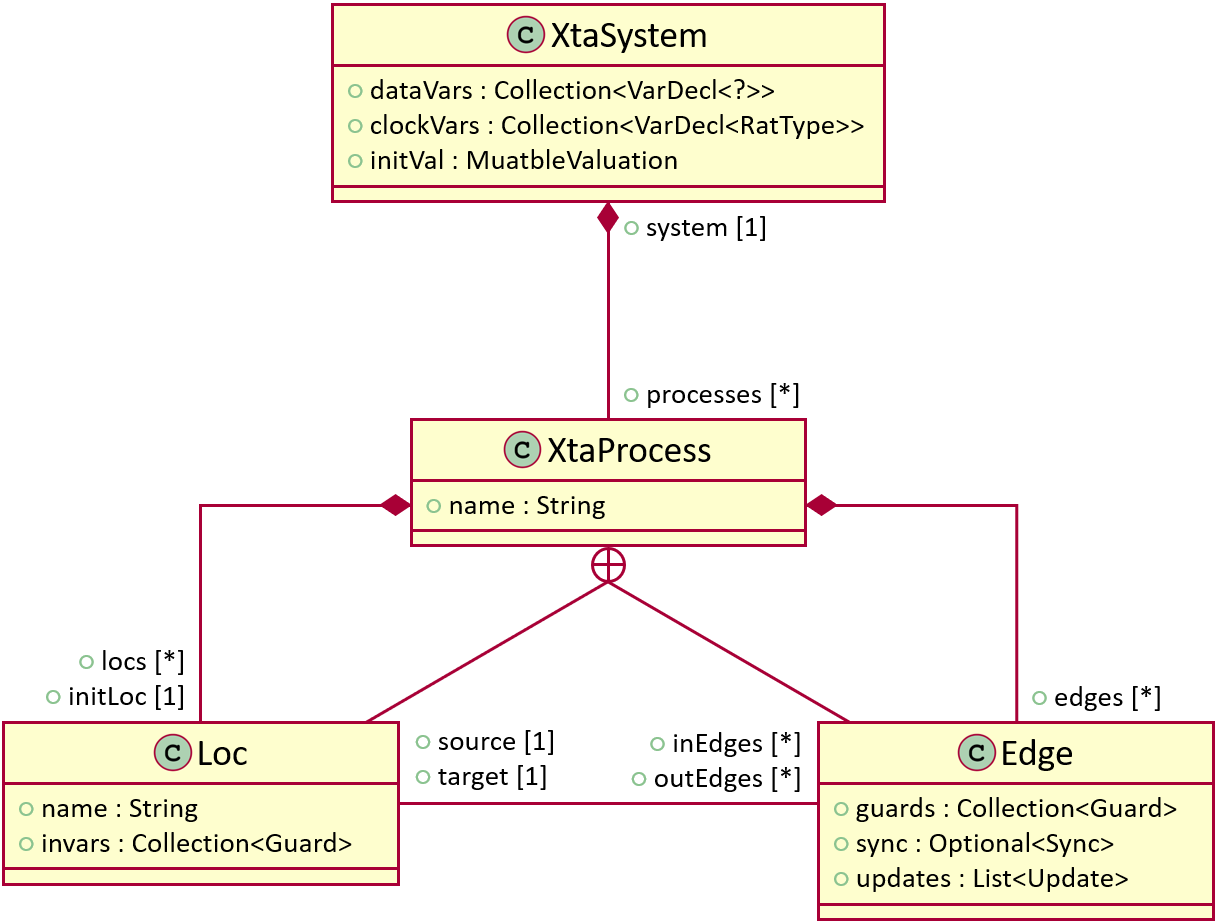
\includegraphics[height=100mm, keepaspectratio]{src/figures/xtasystem-uml.png}
    \caption{Az \textsf{XtaSystem}, \textsf{XtaProcess}, \textsf{Loc}, és \textsf{Edge} osztályok UML osztálydiagramja}
    \label{fig:xtasystem-uml}
\end{figure}

Az \textsf{XtaSystem} osztály időzítettautomata-hálózatok leírására alkalmas, vagyis egy példánya időzített automaták egy $\automatanetwork$ hálózatát írja le. Itt találhatók a hálózat óraváltozói (\textsf{clockVars : Collection<VarDecl<RatType>{}>}) és adatváltozói (\textsf{dataVars : Collection<VarDecl<?>{}>}), utóbbiak kezdeti értékei (\textsf{initVal : MutableValuation}), valamint a hálózatot alkotó $\automatanetwork_i$ időzített automata példányok (\textsf{processes : List<XtaProcess>}).

Az \textsf{XtaProcess} osztály példányai időzített automatákat írnak le. Egy \textsf{XtaProcess} példány rendelkezik névvel (\textsf{name : String}), ismeri az őt tartalmazó hálózatot (\textsf{system : XtaSystem}), valamint tartalmazza a vezérlési helyeit (\textsf{locs : Collection<Loc>}), az éleit (\textsf{edges : Collection<Edge>}) és a kezdő vezérlési helyét (\textsf{initLoc : Loc}).

Az \textsf{XtaProcess} beágyazott osztályai a vezérlési helyeket reprezentáló \textsf{Loc}, valamint az éleket reprezentáló \textsf{Edge}.

Egy \textsf{Loc} objektum tárolja a vezérlési hely nevét (\textsf{name : String}), a belé vezető éleket (\textsf{inEdges : Collection<Edge>}), a belőle kivezető éleket (\textsf{outEdges : Collection<Edge>}), valamint a vezérlési hely invariánsait (\textsf{invars : Collection<Guard>}).

Egy \textsf{Edge} objektum tárolja az él forrás (\textsf{source : Loc}) és cél (\textsf{target : Loc}) vezérlési helyét, az őrfeltételeit (\textsf{guards : Collection<Guard>}), a szinkronizációját (\textsf{sync : Optional<Sync>}) és a változókon végzett frissítéseit (\textsf{updates : List<Update>}).

Az \textsf{XtaSystem}, \textsf{XtaProcess}, \textsf{Loc}, és \textsf{Edge} osztályok UML osztálydiagramja a \ref{fig:xtasystem-uml}. ábrán látható.

\subsection{ARG}
\begin{figure}%[h!]
    \centering
    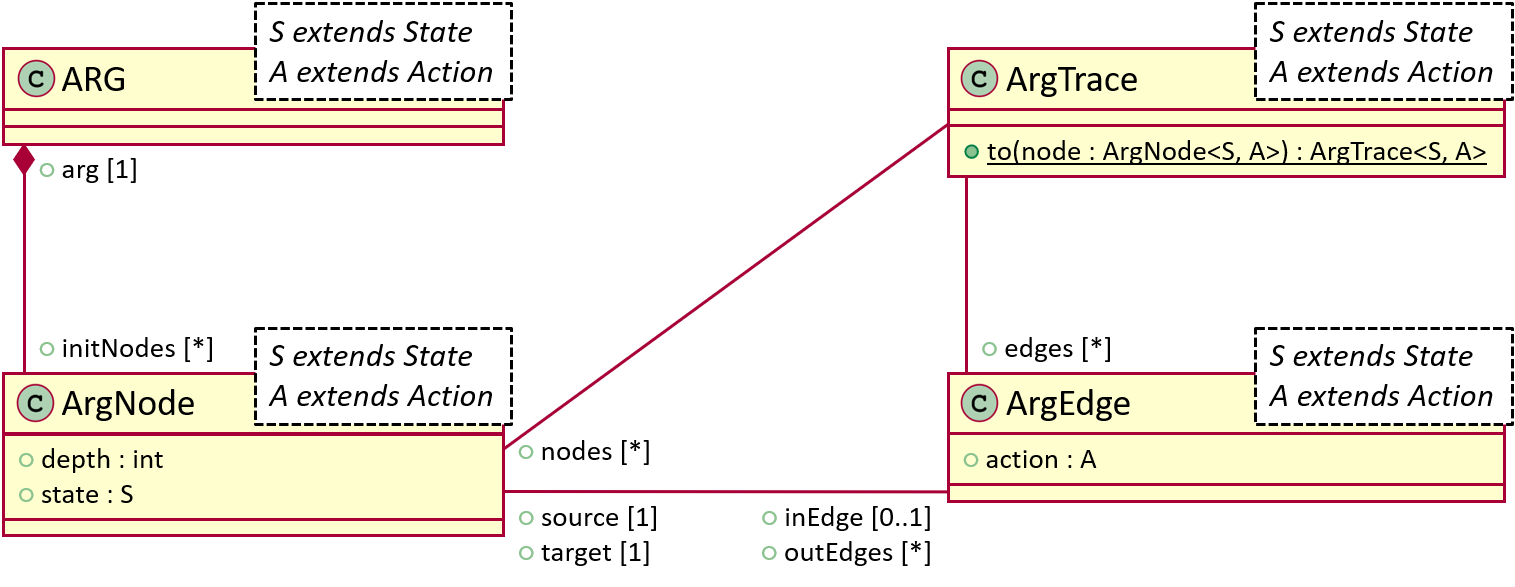
\includegraphics[width=\textwidth, keepaspectratio]{src/figures/arg-uml.png}
    \caption{Az \textsf{ARG}, \textsf{ArgNode}, \textsf{ArgEdge}, és \textsf{ArgTrace} osztályok UML osztálydiagramja}
    \label{fig:arg-uml}
\end{figure}

Egy \textsf{ARG} példány egy absztrakt elérhetőségi gráfot reprezentál. Ez megegyezik a \ref{Theta:felepites}. fejezetben említett ART-vel (absztrakt elérhetőségi fa), és megvalósítja a \ref{def:ASG}. definícióban (ASG) leírtakat.

\textsf{ARG<S extends State, A extends Action>} egy generikus osztály, melynek két típusparamétere az \textsf{S} állapot- és \textsf{A} akciótípus. Esetünkben az \textsf{S} típusparaméter az \textsf{XtaState}, az \textsf{A} típusparaméter pedig az \textsf{XtaAction} lesz. 

Egy \textsf{ARG} gráf \textsf{ArgNode} típusú csúcsokból és \textsf{ArgEdge} típusú élekből áll, de az \textsf{ARG} csak a kezdő csúcsait (\textsf{initNodes : Collection<ArgNode<S, A>{}>}) ismeri közvetlenül.

Egy \textsf{ARG<S, A>} egy hasonlóan generikus \textsf{ArgNode<S, A>} csúcsa ismeri az őt tartalmazó gráfot (\textsf{arg : ARG<S, A>}), tárolja a saját mélységét a fában (\textsf{depth : int}), a belé vezető élt (\textsf{inEdge : Optional<ArgEdge<S, A>{}>}) és a belőle kivezető éleket (\textsf{outEdges : Collection<ArgEdge<S, A>{}>}), valamint a csúcs állapotát (\textsf{state : S}).

Egy \textsf{ARG<S, A>} egy hasonlóan generikus \textsf{ArgEdge<S, A>} éle tárolja forrás (\textsf{source : ArgNode<S, A>}) és cél (\textsf{target : ArgNode<S, A>}) csúcsát, valamint az él akcióját (\textsf{action : A}).

Az \textsf{ArgTrace<S extends State, A extends Action>} osztály egy \textsf{ARG}-beli utat reprezentál, vagyis csúcsok (\textsf{nodes : List<ArgNode<S, A>{}>}) és élek (\textsf{edges : List<ArgEdge<S, A>{}>}) alternáló sorozatát. Az \textsf{ArgTrace} osztály statikus \textsf{to} metódusa a paraméterként kapott \textsf{ArgNode} csúcshoz vezető \textsf{ArgTrace}-t ad vissza.

Az \textsf{ARG}, \textsf{ArgNode}, \textsf{ArgEdge}, és \textsf{ArgTrace} osztályok UML osztálydiagramja a \ref{fig:arg-uml}. ábrán látható.

\subsection{XtaState}

\begin{figure}%[h!]
    \centering
    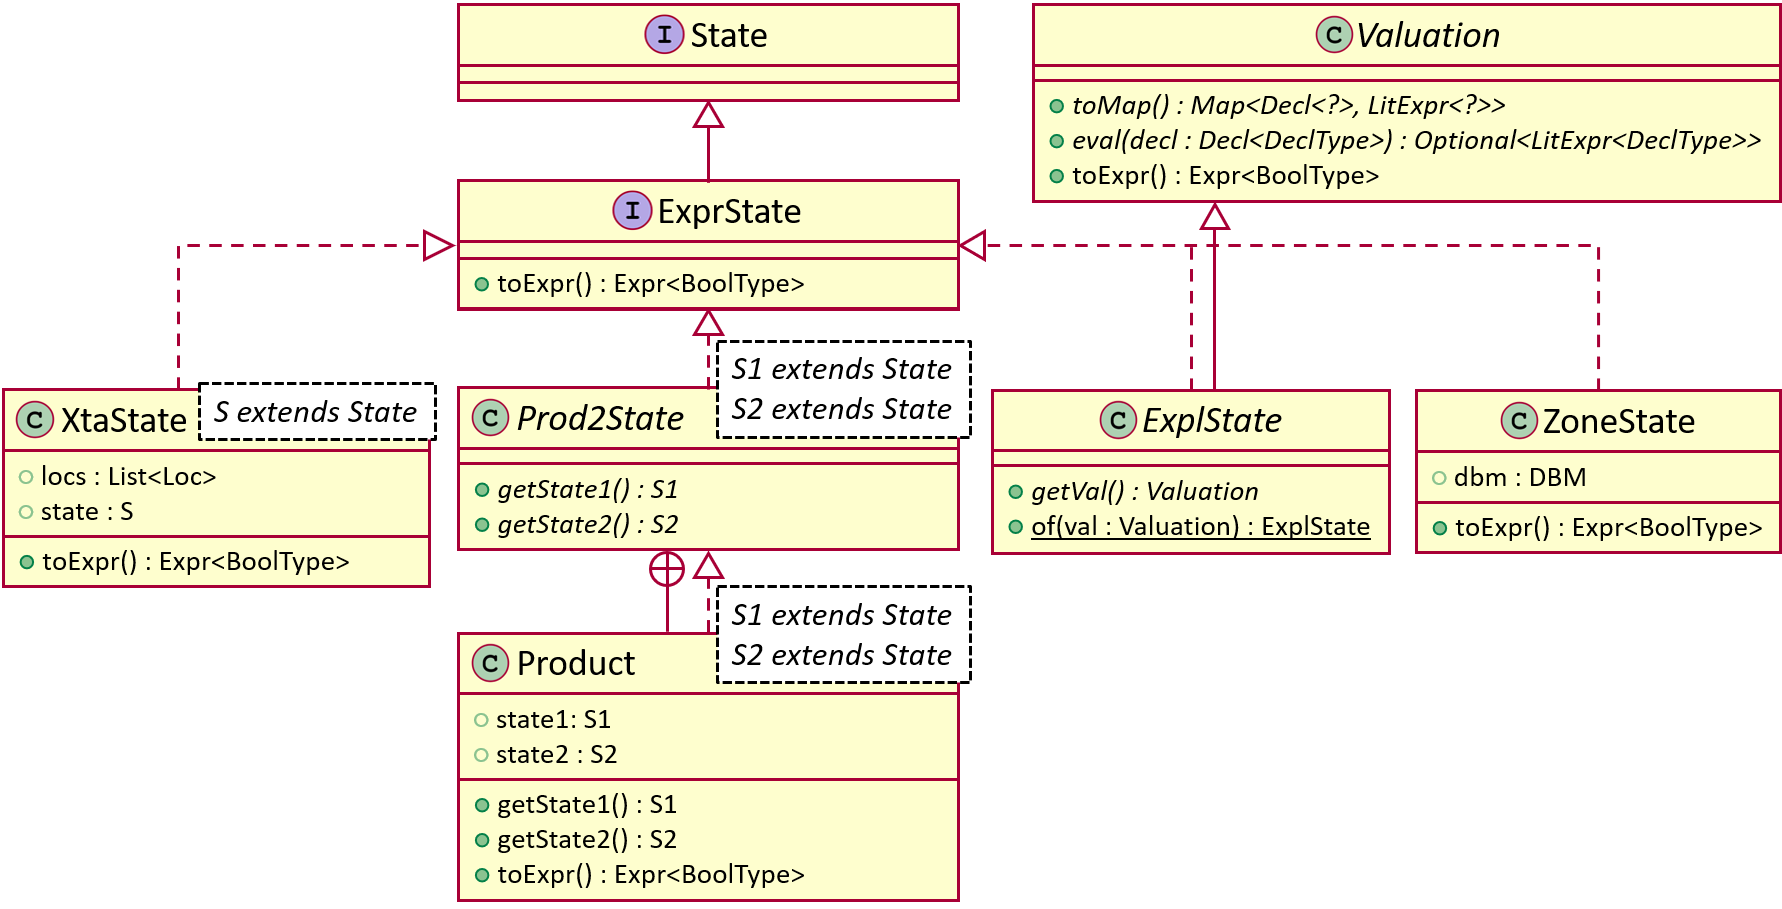
\includegraphics[width=\textwidth, keepaspectratio]{src/figures/xtastate-uml.png}
    \caption{Az \textsf{XtaState} és kapcsolódó osztályok UML osztálydiagramja}
    \label{fig:xtastate-uml}
\end{figure}

Az \textsf{XtaState<S extends State>} generikus osztály egy \textsf{ArgNode} állapotát írja le. Tárolja az állapotban aktív vezérlési helyeket (\textsf{locs : List<Loc>}), valamint egy állapotot (\textsf{state : S}), amely esetünkben két állapot szorzata (\textsf{Prod2State.Product}). Az állapotot ugyanis egy explicit állapot (\textsf{ExplState}) és egy zónaállapot (\textsf{ZoneState}) együtt határozzák meg. Előbbi az értékváltozókra vonatkozó kényszereket (\textsf{Valuation} alakban), míg utóbbi a zónákat, vagyis az óraváltozókra vonatkozó kényszereket (\textsf{DBM} alakban) tartalmazza.

Az imént említett osztályok (\textsf{XtaState}, \textsf{Prod2State.Product}, \textsf{ExplicitState}, \textsf{ZoneState}) mind megvalósítják az \textsf{ExprState} interfészt, vagyis definiálniuk kell a \textsf{toExpr} függvényt. Ez a függvény az objektumban lévő kényszereket egy \textsf{Expr<BoolType>} objektummá alakítja.

Az \textsf{XtaState} és kapcsolódó osztályok UML osztálydiagramja a \ref{fig:xtastate-uml}. ábrán látható.

\subsection{XtaAction}
\begin{figure}%[h!]
    \centering
    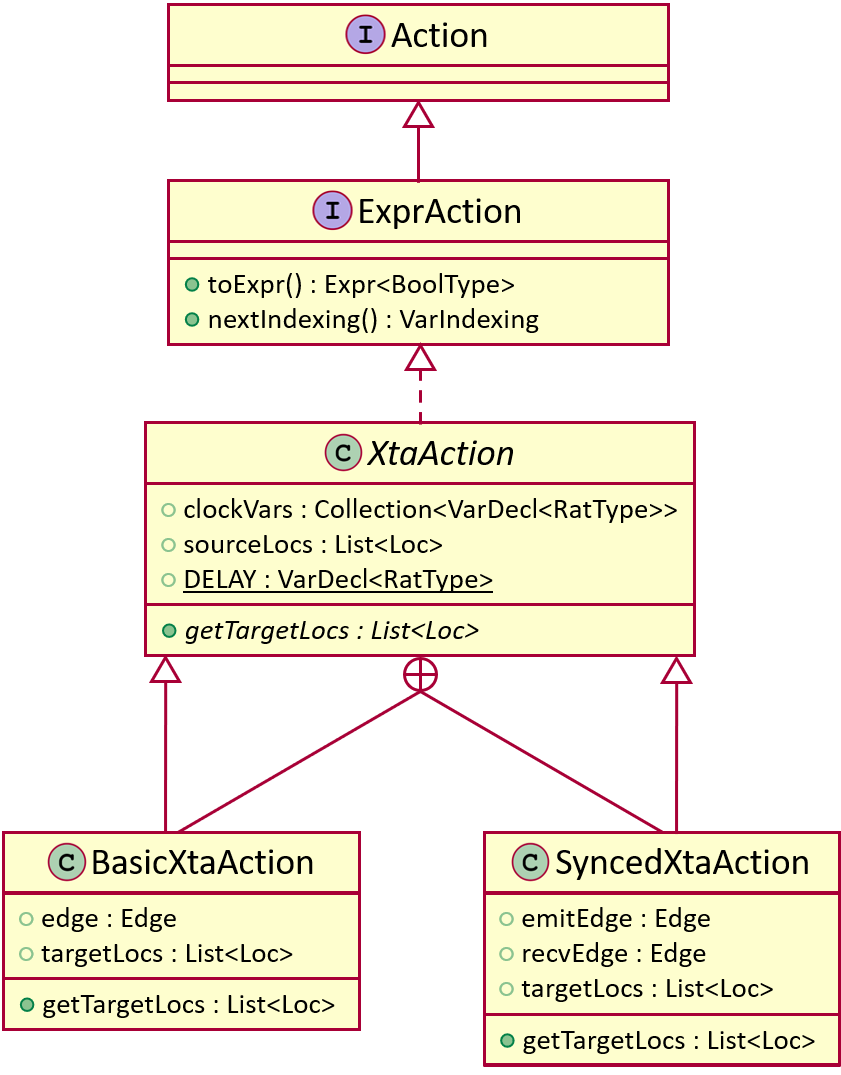
\includegraphics[height=120mm, keepaspectratio]{src/figures/xtaaction-uml.png}
    \caption{Az \textsf{XtaAction} és kapcsolódó osztályok UML osztálydiagramja}
    \label{fig:xtaaction-uml}
\end{figure}

Az \textsf{XtaAction} osztály egy \textsf{ArgEdge} akcióját írja le. Ismeri az óraváltozókat (\textsf{clockVars : Collection<VarDecl<RatType>{}>}), illetve a forrás (\textsf{sourceLocs : List<Loc>}) és cél (\textsf{targetLocs : List<Loc>}) állapotban aktív vezérlési helyeket. Itt található továbbá a statikus, \textsf{VarDecl<RatType>} típusú \textsf{DELAY} adattag, amely azt a változót reprezentálja, amely megadja, hogy egy állapotban mennyit várakozik a rendszer.

Az \textsf{XtaAction} osztály absztrakt, két leszármazottal: a \textsf{BasicXtaAction} osztály szinkronizáció nélküli átmeneteket, míg a \textsf{SyncedXtaAction} osztály szinkronizáló átmeneteket reprezentál. A \textsf{BasicXtaAction} osztály egy időzített automata egyetlen élére (\textsf{edge : Edge}) vonatkozik, míg a \textsf{SyncedXtaAction} osztály egyaránt ismeri a szinkronizációt küldő (\textsf{emitEdge : Edge}) és fogadó (\textsf{recvEdge : Edge}) élt.

Az \textsf{XtaState}-nél bemutatotthoz hasonlóan az \textsf{XtaAction} is megvalósítja az \textsf{ExprAction} interfészt, vagyis definiálja az ott deklarált \textsf{toExpr} metódust. Ennek a működése megegyezik az \textsf{ExprState}-nél leírttal.

\subsection{Típusok}

\begin{figure}%[h!]
    \centering
    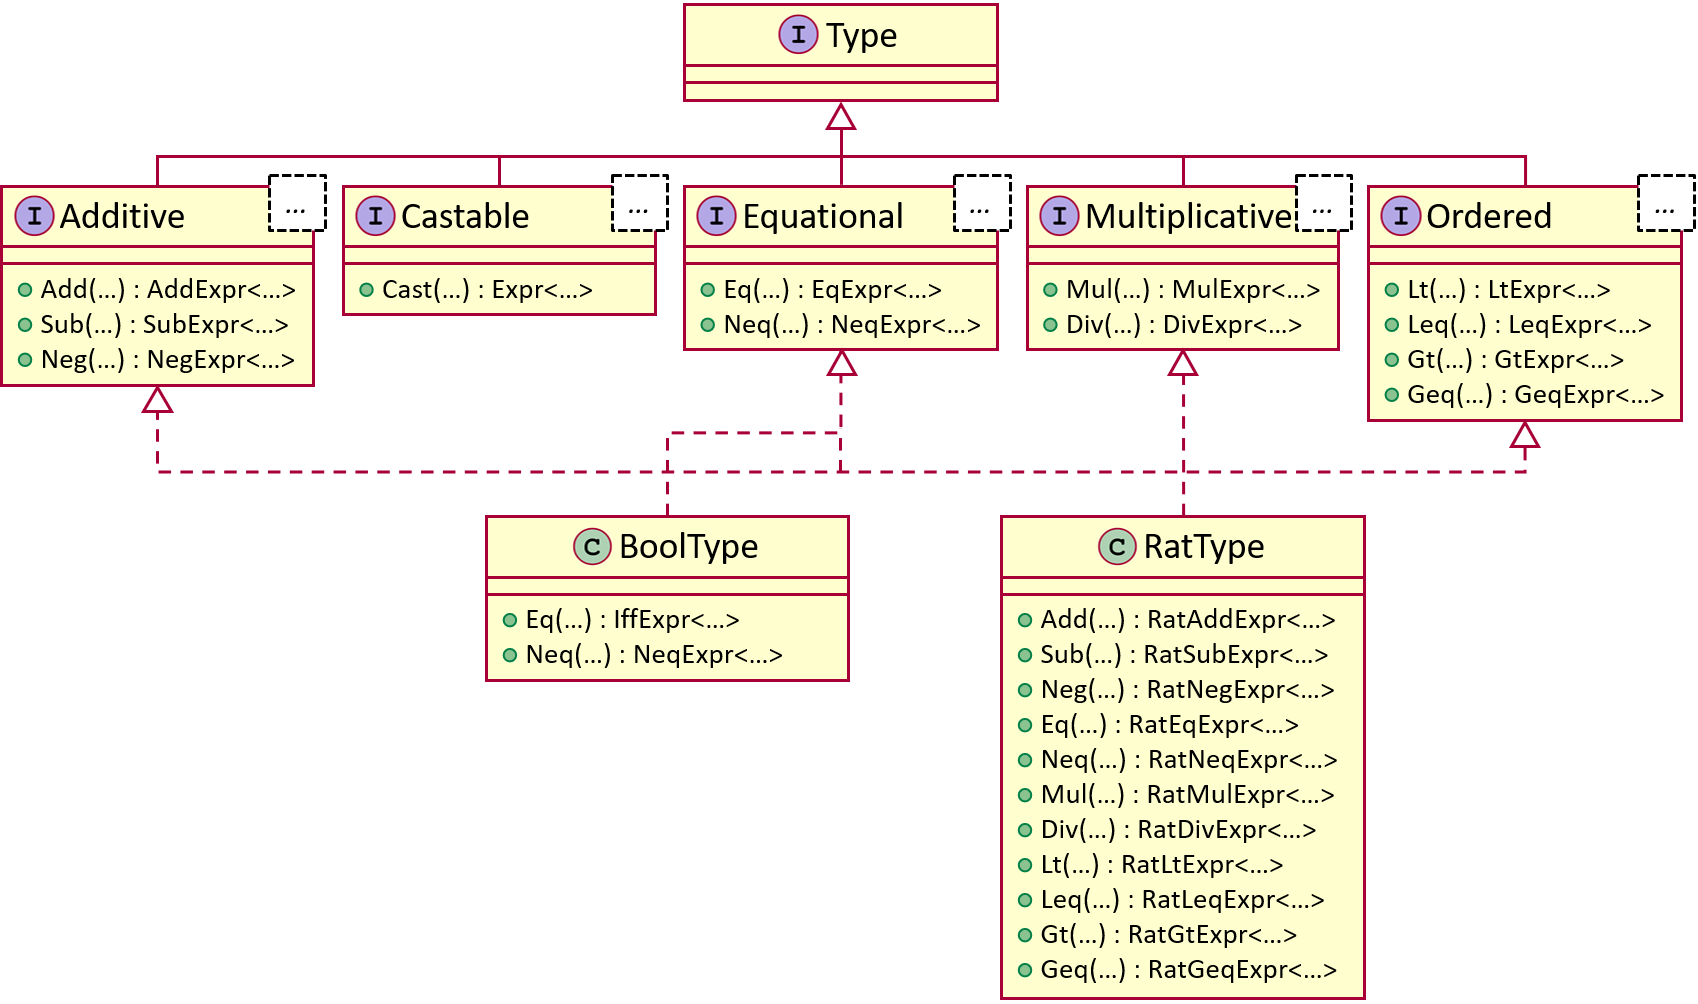
\includegraphics[width=\textwidth, keepaspectratio]{src/figures/type-uml.png}
    \caption{Típusok a Theta-ban}
    \label{fig:type-uml}
\end{figure}

A Theta típusainak őse a \textsf{Type} interfész. Ezt valósítják meg az \textsf{Additive}, \textsf{Castable}, \textsf{Equational}, \textsf{Multiplicative} és \textsf{Ordered} interfészek (értelemszerű függvénydeklarációkkal), amelyek implementálása azt jelenti, hogy az adott típuson értelmezhetők a névben szereplő műveletek (összeadás, kivonás, negálás; típuskonverzió; egyenlőségvizsgálat; szorzás, osztás; összehasonlítás).

A \textsf{BoolType} a logikai típust, a \textsf{RatType} a racionális típust jelöli. Ezen osztályok egyszerűsített UML osztálydiagramja látható a \ref{fig:type-uml}. ábrán.

\subsection{Változók}
\begin{figure}%[h!]
    \centering
    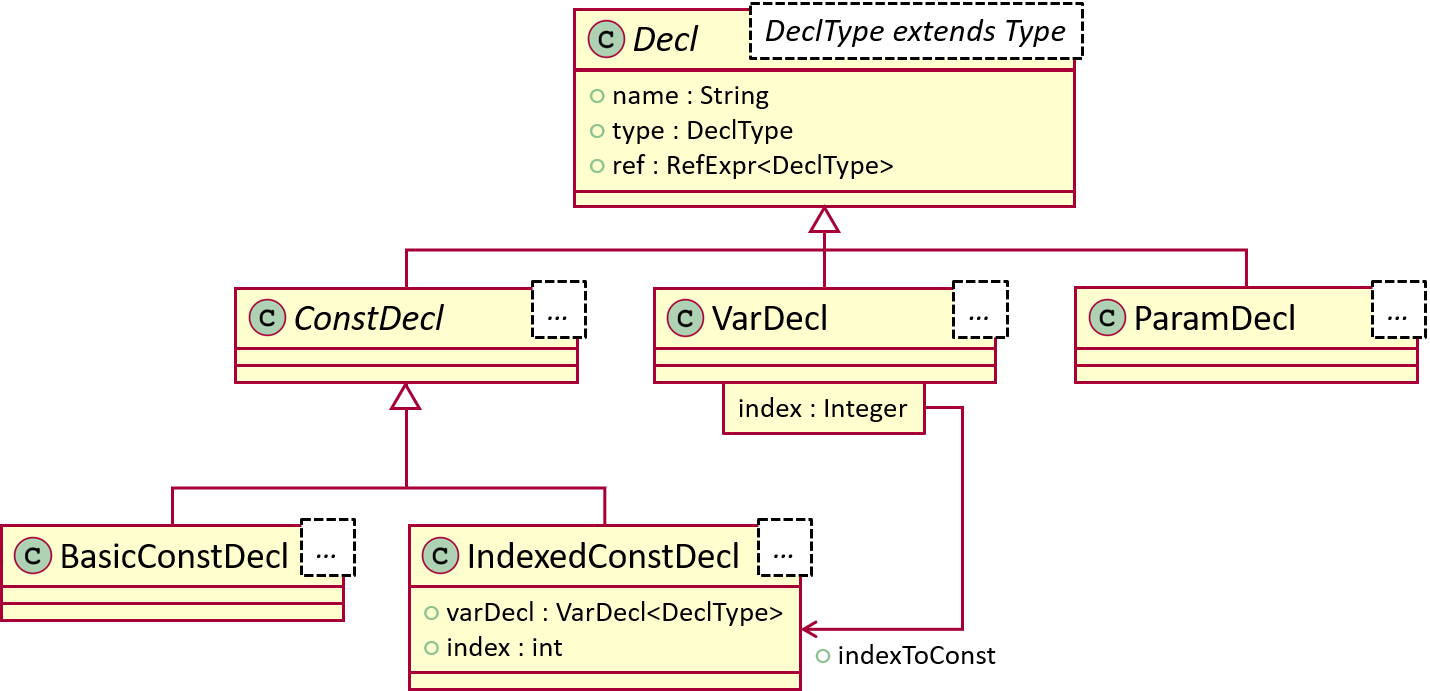
\includegraphics[width=\textwidth, keepaspectratio]{src/figures/decl-uml.png}
    \caption{Deklarációk a Theta-ban}
    \label{fig:decl-uml}
\end{figure}

A Theta-ban háromféle dolgot deklarálhatunk: konstanst, változót és paramétert. Minden deklaráció a generikus \textsf{Decl<DeclType extends Type>} ősből származik, amely tartalmazza a deklaráció nevét (\textsf{name : String}), típusát (\textsf{type : DeclType}) és referenciáját (\textsf{ref : RefExpr<DeclType>}). Minden \textsf{Decl}-ből leszármazó specifikus deklaráció is \textsf{Decl}-lel megegyezően generikus.

Kétféle konstansdeklaráció lehetséges: \textsf{BasicConstDecl} és \textsf{IndexedConstDecl}. Utóbbi egy változó adott indexelésére vonatkozik, ennek megfelelően egy változódeklarációt (\textsf{varDecl : VarDecl<DeclType>}) és egy indexet (\textsf{index : int}) tartalmaz.

A változódeklaráció (\textsf{VarDecl}) tartalmaz egy hozzárendelést (\textsf{indexToConst : Map<Integer, IndexedConstDecl<DeclType>{}>}), amely egy indexeléséhez egy indexelt konstansdeklarációt rendel.

A \textsf{VarIndexing} osztály változókhoz rendel indexértékeket, így alkalmas annak a tárolására, hogy egy kifejezésben melyik változó milyen indexszel szerepel. Az alapértelmezett \textsf{defaultIndex : int} indexhez képest tárolja a változók indexeltolását (offszet) a \textsf{varToOffset : Map<VarDecl<?>, Integer>}-ben. A \textsf{get} függvény adja meg egy adott \textsf{varDecl} változóhoz tartozó indexet, melynek visszatérési értéke \textsf{defaultIndex} és \textsf{varDecl} \textsf{varToOffset}-ben tárolt offszetjének összege.

A deklarációkat leíró osztályok UML osztálydiagramja látható a \ref{fig:decl-uml}. ábrán.

\subsection{Kifejezések}

\begin{figure}%[h!]
    \centering
    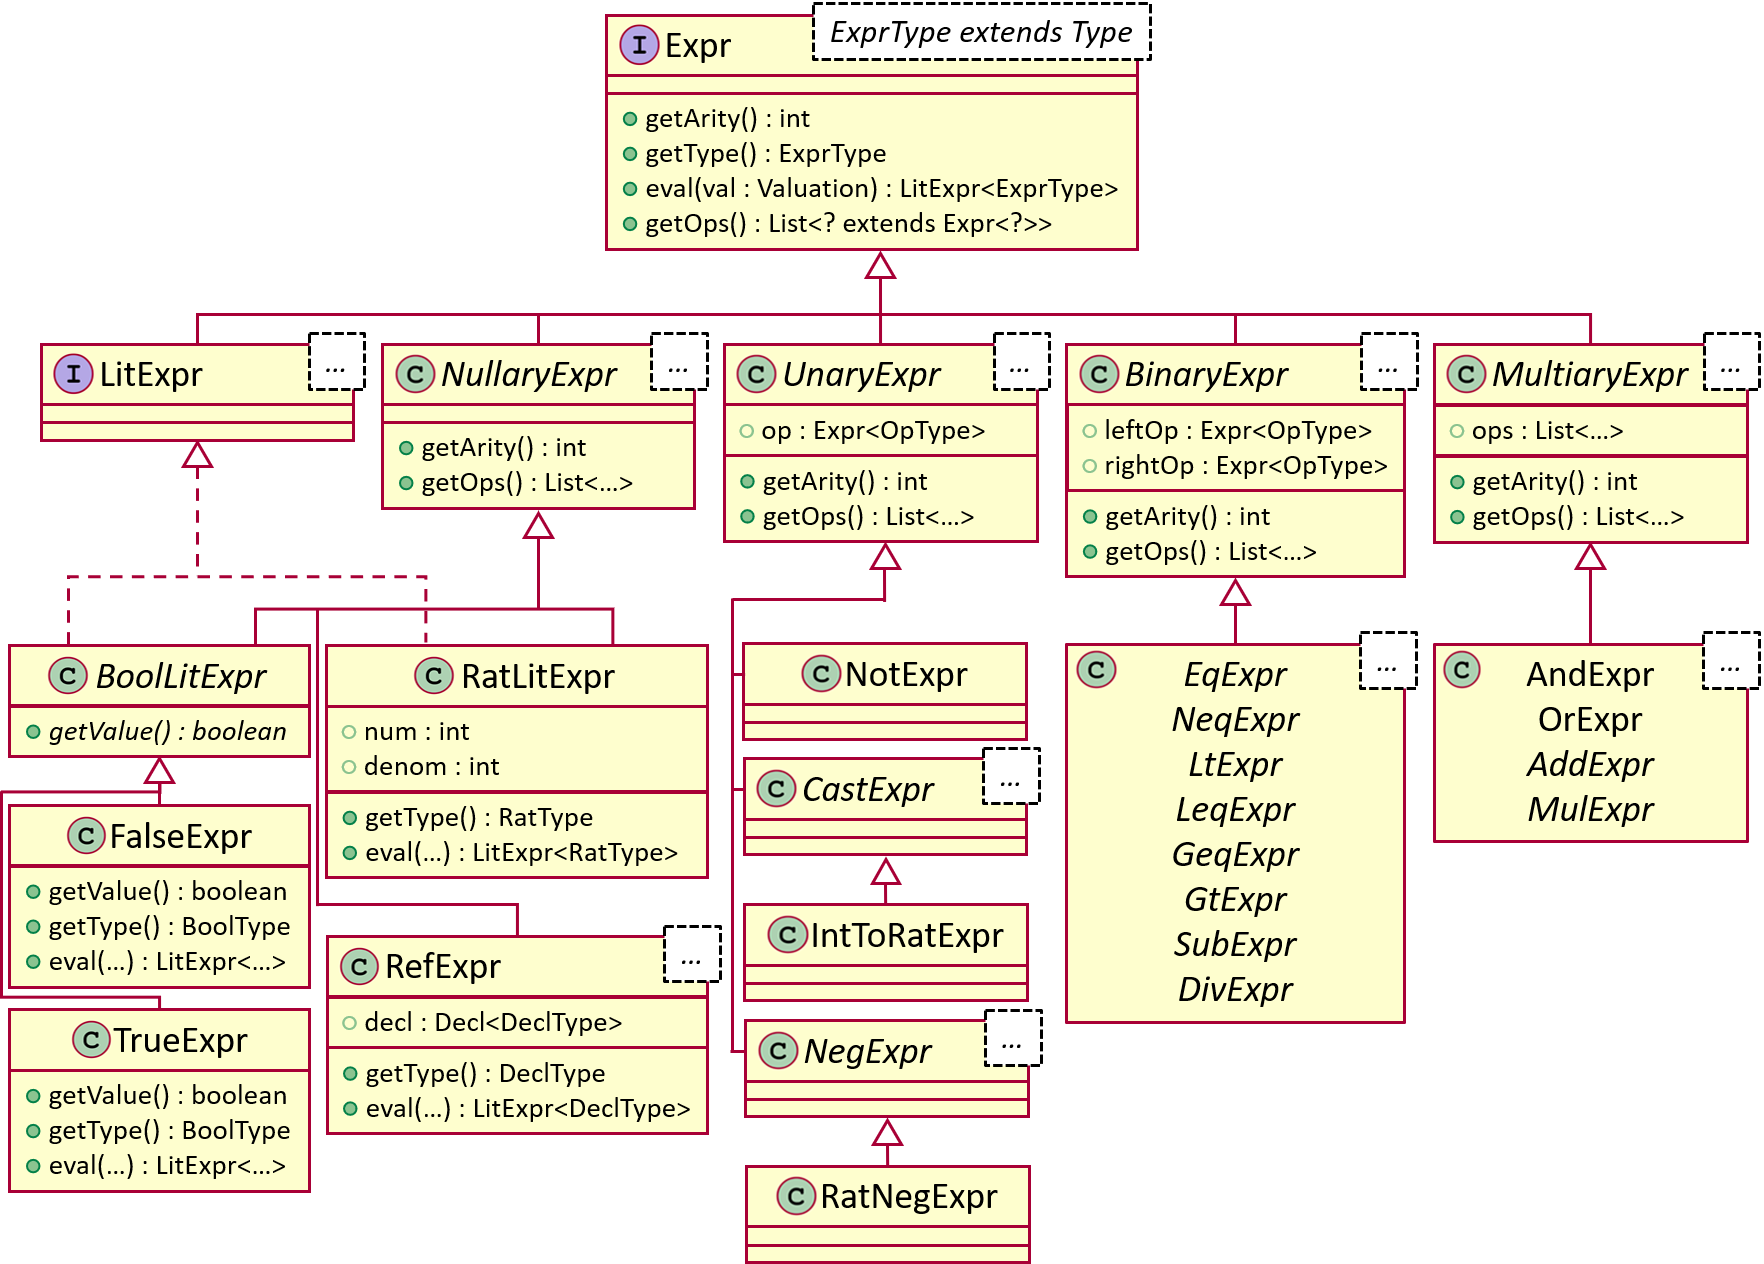
\includegraphics[width=\textwidth, keepaspectratio]{src/figures/expr-uml.png}
    \caption{Kifejezések a Theta-ban}
    \label{fig:expr-uml}
\end{figure}

A Theta kifejezéseinek őse a generikus \textsf{Expr} interfész, melynek \textsf{ExprType extends Type} típusparamétere a kifejezés értékének típusa. A kifejezés típusát a \textsf{getType}, aritását a \textsf{getArity}, operandusait a \textsf{getOps} metódus adja meg. A kifejezés kiértékelésére az \textsf{eval} metódus szolgál, melynek \textsf{Valuation} típusú \textsf{val} paramétere deklarációkhoz rendel literál kifejezéseket, visszatérési értéke pedig kifejezés értékét reprezentáló literál. A \textsf{val} paraméter hordozza az információt, hogy a kifejezésben található deklarációreferencia változók (\textsf{RefExpr}) helyére milyen literál értéket (\textsf{LitExpr}) kell behelyettesíteni.

Az \textsf{Expr} interfészt megvalósító absztrakt osztályok a kifejezések aritása szerinti ősosztályok (\textsf{NullaryExpr}, \textsf{UnaryExpr}, \textsf{BinaryExpr}, \textsf{MultiaryExpr}), ezekből származnak le a konkrét műveleteket reprezentáló kifejezésosztályok (típusspecifikus műveletek esetén (pl. negálás: \textsf{NegExpr}) ebből még további típusspecifikus osztályok származnak le (pl. racionális negálás: \textsf{RatNegExpr})).

A 0 aritású kifejezések lehetnek literálok, vagyis típusspecifikus értékek, vagy deklarációreferenciák, vagyis egy deklaráció konkrét használati esetei. Egy deklarációreferencia által referált deklarációhoz egy \textsf{Valuation} objektum rendel literál értéket az \textsf{eval} metódusával.

A \textsf{PathUtils} osztály statikus \textsf{unfold} metódusa egy \textsf{expr : Expr} kifejezést és egy \textsf{varIndexing : VarIndexing} változóindexelést kap paraméterül. A visszatérési értéke egy olyan kifejezés, amelyben az \textsf{expr}-beli \textsf{VarDecl}-re referáló \textsf{RefExpr}-ek a megfelelő \textsf{varIndexing}-beli indexszel vannak indexelve.

A kifejezéseket bemutató egyszerűsített UML osztálydiagram a \ref{fig:expr-uml}. ábrán látható. A \textsf{BinaryExpr} és \textsf{MultinaryExpr} osztályok ősei a könnyebb áttekinthetőség érdekében tömörítve láthatók, a további típusspecifikus leszármazottak nem szerepelnek az ábrán.

\subsection{Solver}
A Theta által használt SMT megoldók a \textsf{Solver} interfészen keresztül érhetők el. Az \textsf{add} függvénnyel adhatunk meg új, \textsf{Expr<BoolType>} típusú kényszereket. A \textsf{pop} metódus eltávolítja a legutóbbi \textsf{push} óta hozzáadott kényszereket.

A \textsf{check} metódus megvizsgálja a probléma kielégíthetőségét, amit egy \textsf{SolverStatus} enumként ad vissza, amelynek az \textsf{isSat} metódusa megadja a kielégíthetőség logikai értékét.

Amennyiben a probléma kielégíthető, a \textsf{getModel} metódus megadja azt a \textsf{Valuation} objektumot, amely tartalmazza a megoldott SMT probléma változóinak értékeit, vagyis a probléma megoldását.

\subsection{Vizualizáció}
A Theta egyaránt támogatja belső gráfreprezentációk kiírását dot formátumba, illetve közvetlen kirajzolását számos kiterjesztésű képfájlba a Graphviz\footnote{\url{http://www.graphviz.org/}} eszközzel.

A Theta belső gráfreprezentációja a \textsf{Graph} osztály, amely egy azonosítóval (\textsf{id : String}), címkével (\textsf{label : String}), valamint csúcsokkal (\textsf{nodes : Map<String, Node>}) és élekkel (\textsf{edges : Collection<Edge>}) rendelkezik. Az \textsf{addNode} metódus egy új csúcsot ad hozzá a gráfhoz, egyedi azonosítóval (\textsf{id : String}) és tetszőleges attribútumokkal (\textsf{attributes : NodeAttributes}). Az \textsf{addEdge} metódus élt ad hozzá a gráfhoz két adott azonosítójú (\textsf{sourceId, targetId : String}) csúcs közé, tetszőleges attribútumokkal (\textsf{attributes : EdgeAttributes}).

Az attribútum osztályokban (\textsf{NodeAttributes, EdgeAttributes}) található tulajdonságok megfeleltethetők a dot nyelvben lévő csúcs- és éltulajdonságoknak.\footnote{\url{https://www.graphviz.org/pdf/dotguide.pdf}} Egy tetszőleges gráf előállításához tehát csupán megfelelő \textsf{NodeAttributes} és \textsf{EdgeAttributes} objektumokat kell átadnunk egy \textsf{Graph} objektum \textsf{addNode} és \textsf{addEdge} függvényének.

Egy \textsf{Graph} objektumot a \textsf{GraphvizWriter} osztály \textsf{writeFile} függvényével írhatunk ki számos formátumú fájlba. A függvény paraméterlistája egy \textsf{Graph} objektumból, a kimeneti fájl nevéből és egy fájlformátumot leíró \textsf{GraphvizWriter.Format} enumból áll.

\subsection{Logger}
A Theta beépítetten támogatja a naplózást (logolást) is, a \textsf{Logger} interfészen keresztül. A \textsf{Logger.Level} enummal határozható meg az adott logolás prioritása. A \textsf{write} metódus segítségével írhatunk a logba, adott prioritással.

\section{A tesztgenerálás megvalósítása} \label{megvalositas}

A tesztgenerálás megvalósítására külön alprojektet (\textsf{xta-testgeneration}) és package-et (\textsf{hu.bme.mit.theta.xta.testgeneration}) hoztam létre.

Az \textsf{XtaCli} osztályt kiegészítettem egy további parancssori kapcsoló (\texttt{-{}-testgen} vagy \texttt{-t}) kezelésével (\textsf{testGeneration}). Amennyiben ezzel indítják a programot, a \textsf{run} metódus meghívja a \textsf{XtaTestGenerator} osztály \textsf{generateTests} metódusát, amely egy időzített teszttel (\textsf{Set<? extends XtaTest<?, ?>{}>}) tér vissza.

Ezt a tesztkészletet ezután a \textsf{printTests} metódussal kiíratjuk a konzolra, a \textsf{visualizeTests} metódussal pedig kirajzoltatjuk fájlokba. Előbbi az \textsf{XtaTestPrinter}, utóbbi az \textsf{XtaTestVisualizer} osztályt használja.

\subsection{XtaTest}
Az \textsf{XtaTest<S extends XtaState<? extends State>, A extends XtaAction>} osztály egy példánya reprezentál egy időzített tesztesetet. Egy tesztesetet egy név (\textsf{name : String}), egy ARG-beli útvonal (\textsf{trace : ArgTrace<S, A>}), valamint az időzítések (\textsf{delays : List<Double>}) határoznak meg. A \textsf{getTotalTime} metódus megadja a \textsf{delays}-beli várakozások összegét, a \textsf{getLocs} metódus pedig a teszt által érintett vezérlési helyek halmazát.

\subsection{XtaTestGenerator}
A tesztgenerálást egy \textsf{XtaSystem} objektum által leírt $\automatanetwork$ automatahálózathoz egy \textsf{ARG} objektum alapján az \textsf{XtaTestGenerator} osztály végzi, egy \textsf{Solver} és egy \textsf{Logger} objektum felhasználásával.

A \textsf{generateTests} metódus valósítja meg az \ref{GenerateTests}. algoritmust, vagyis szélességi bejárással addig generál új teszteket (\textsf{generateTest}), amíg a $\networktestset$ tesztkészlet le nem fedi az $\automatanetwork$ automatahálózat összes vezérlési helyét.

A \textsf{generateTest} metódus az ARG egy konkrét csúcsához vezető $\networktest$ tesztesetet generál a \ref{GenerateTest}. algoritmusban leírtak szerint. A paraméterként kapott \textsf{ArgNode}-hoz az \textsf{ArgTrace} osztály statikus \textsf{to} metódusával generál \textsf{ArgTrace}-t. A generált útvonalú teszteset időzítését a \textsf{calculateDelays} metódus végzi.

A \textsf{calculateDelays} metódus valósítja meg a \ref{CalculateDelays}. algoritmusban leírtakat, vagyis egy $\networktest$ tesztesetnek kiszámolja a $\hat{t}(\networktest)$ időzítését. Először összeállítja a megoldandó SMT problémát, majd megoldja azt a \textsf{Solver} objektum felhasználásával, végül megkísérli javítani a kapott megoldást. A problémát adó kényszerek a következő metódushívásokkal állnak elő:
\begin{enumerate}
    \item \textsf{addInitialClockConstraint}: a kezdő várakozások meg kell, hogy egyezzenek az óraváltozók kezdeti értékével,
    \item \textsf{addInitialNodeConstraint}: a kezdőállapotot leíró kényszerek,
    \item \textsf{addTraceConstraints}: a teszteset éleit és újabb állapotait leíró kényszerek,
    \item \textsf{addSumOfDelaysConstraint}: új változó deklarálása $time(\networktest) = \sum\limits_{i = 1}^{|\networktest|} \hat{t}_i$-re.
\end{enumerate}

Az \textsf{addInitialClockConstraints} függvény az \textsf{XtaSystem} objektum \textsf{getClockVars} metódusával lekéri $\automatanetwork$ összes óraváltozóját, valamint létrehoz egy \textsf{delayRef : RefExpr<RatType>} referenciát az \textsf{XtaAction} osztály statikus \textsf{DELAY} változójára. Végigiterál az összes \textsf{cv} óraváltozón, létrehoz rájuk egy \textsf{clockVarRef : RefExpr<RatType>} referenciát a \textsf{RefExpr} osztály statikus \textsf{to} függvényével, majd egy listába teszi a \textsf{delayRef} és \textsf{clockVarRef} közti egyenlőség kifejezéseket, amelyeket az \textsf{EqExpr} osztály statikus \textsf{create2} függvényével hoz létre. Az \textsf{AndExpr} osztály statikus \textsf{to} függvényével ÉS kapcsolatba fűzi az imént létrehozott egyenlőség kifejezéseket, majd a \textsf{PathUtils} osztály statikus \textsf{unfold} függvényével minden változót 0-val indexel. Az így kapott \textsf{Expr<BoolType>} kifejezést adja hozzá a \textsf{Solver} objektumhoz.

Az \textsf{addInitialNodeConstraint} függvény a paraméterként kapott \textsf{ArgTrace} objektum kezdő \textsf{ArgNode}-jának állapotát alakítja \textsf{Expr<BoolType>} objektummá a \textsf{toExpr} metódus segítségével, majd a kifejezés változóit 0-val indexeli a \textsf{PathUtils} osztály \textsf{unfold} függvényével. Az így kapott \textsf{Expr<BoolType>} kifejezést adja hozzá a \textsf{Solver} objektumhoz.

Az \textsf{addTraceConstraints} függvény végigiterál a paraméterként kapott \textsf{ArgTrace} objektum további csúcsain és élein, és azok \textsf{XtaState} állapotát illetve \textsf{XtaAction} élét azok \textsf{toExpr} metódusával \textsf{Expr<BoolType>} kifejezéssé alakítja. Ezen kifejezések megfelelően indexelt alakját adja hozzá a \textsf{Solver} objektumhoz. A megfelelő indexelés megállapításához a paraméterként kapott \textsf{indexing : List<VarIndexing>} listához mindig hozzáad egy újabb elemet, amelyet úgy kap meg, hogy a legutóbbi \textsf{VarIndexing} elemhez hozzáadja az \textsf{XtaAction} objektum \textsf{nextIndexing} metódusa által visszaadott indexelést.

Az \textsf{addSumOfDelays} függvény egy új \textsf{totalTime : ConstDecl<RatType>} racionális típusú deklarációt hoz létre \texttt{\_\_total\_\_time\_\_} névvel, illetve egy erre mutató \textsf{totalTimeRef : RefExpr<RatType>} referenciát. Az \textsf{XtaAction} osztály statikus \textsf{DELAY} adattagjára is létrehoz egy \textsf{delayRef : RefExpr<RatType>} referenciát. Ezután összegyűjti a teszt összes lépéséhez tartozó \textsf{delayRef}-indexelést a \textsf{delayRefs : List<Expr<RatType>{}>} listába a \textsf{PathUtils} osztály statikus \textsf{unfold} függvényének segítségével. Végül hozzáadja a \textsf{Solver} objektumhoz a \textsf{delayRefs}-beli elemek összegének és \textsf{totalTimeRef}-nek az egyenlőségét az \textsf{EqExpr} és \textsf{AddExpr} osztályok statikus \textsf{create2} függvényének segítségével.

Miután a \textsf{Solver} objektum megoldást talált a \textsf{calculateDelays} által összeállított problémára, a \textsf{reduceDelays} megkísérli javítani azt $time(\networktest)$ csökkentésével.

A \textsf{reduceDelays} metódus addig szorítja egyre szűkebb \textsf{min, max : RatLitExpr} korlátok közé \textsf{totalTime} értékét, amíg az intervallum már olyan szűk, hogy nincs értelme további javítási próbálkozásnak. Az alsó \textsf{min} korlát kezdetben 0, míg a felső \textsf{max} korlát kezdetben az eredeti időzítés \textsf{totalTime} értéke.

A ciklus minden lépésben \textsf{min} és \textsf{newMax} közé próbálja szorítani a teszt teljes idejét egy \textsf{totalTime} $\leq$ \textsf{newMax} kényszer hozzáadásával. \textsf{newMax} értéke minden esetben a \textsf{min} és \textsf{max} által meghatározott intervallum közepe, vagyis \textsf{min} $+$ (\textsf{max} $-$ \textsf{min}) $/ 2$.

Amennyiben van \textsf{newMax}-nál kisebb megoldás, \textsf{max} új értéke az új megoldás \textsf{totalTime} értéke lesz, amennyiben pedig nincs, \textsf{min} új értéke lesz \textsf{newMax} előző értéke. \textsf{newMax} értékét minden iteráció végén frissítjük.

A ciklus addig javítja tovább az időzítést, amíg a \textsf{max} - \textsf{newMax} $\geq 0,5$ feltétel teljesül. A \textsf{reduceDelays} metódus által visszaadott \textsf{Valuation} objektumból az \textsf{extractDelays} metódus állítja elő az időzítések sorozatát, amellyel a \textsf{calculateDelays} függvény visszatér.

\subsection{XtaTestPrinter}
Az \textsf{XtaTestPrinter} osztály \textsf{XtaTest} objektumok kiírására alkalmas. A statikus \textsf{printTests} metódus egy \textsf{Logger} objektumot és tesztek halmazát kapja paraméterül, és utóbbi minden elemére meghívja a \textsf{printTest} metódust, amely egy teszt kiírását végzi.

A \textsf{printTest} metódus minden lépésben kiírja az \textsf{XtaState} objektumot a Theta alapértelmezett formátumában, valamint az adott lépésben eltöltött időt, majd az \textsf{XtaAction} objektumot, szintén a Theta alapértelmezett formátumában. Egy teszt kiírását a teszt teljes idejének kiírásával zárja.

\subsection{XtaTestVisualizer}
Az \textsf{XtaTestVisualizer} osztály \textsf{XtaTest} objektumok fájlba kirajzolására alkalmas. A statikus \textsf{visualizeTests} metódus tesztek halmazát kapja paraméterül, és annak minden elemére meghívja a \textsf{visualizeTest} metódust, amely egy teszt fájlba kirajzolását végzi.

A \textsf{visualizeTest} metódus a paraméterként kapott \textsf{XtaTest} objektumból előállít egy \textsf{Graph} objektumot, amelyre meghívja a \textsf{GraphvizWriter} osztály \textsf{writeFile} metódusát.

A kimeneti képen minden automata lefutását szeretnénk együttesen látni, vagyis minden automata egy oszlopba rendezett láncgráf, ahol felülről lefelé telik az idő. A jobb áttekinthetőség érdekében minden automatánál csak akkor jelenítünk meg egy aktív vezérlési helyet, ha az éppen megváltozott.

A teszt minden lépésében minden aktív vezérlési helyhez kirajzolunk egy új csúcsot, amibe az adott automata előző aktív vezérlési helyéből vezet él. Ez a csúcs viszont csak akkor lesz látható, ha eltér az adott automata előző aktív vezérlési helyétől, egyébként láthatatlan lesz, amihez a Graphviz \texttt{invis} attribútumát használjuk. A csúcsokon megjelenítjük, hogy abban a lépésben mennyi ideig várakozott a teszt.
% TeXstudio spellcheck 2020-12-10 16:39

\chapter{Kiértékelés} \label{esettanulmany}

Ebben a fejezetben a Fischer-protokollon keresztül részletesen bemutatom a megvalósított teljes tesztgenerálási folyamatot (\ref{fischer}. fejezet) és a megoldásomon végzett mérések eredményeit (\ref{meresek}. fejezet).

\section{Fischer-protokoll} \label{fischer}

A tesztgenerálási folyamatot részletesen a Fischer-féle kölcsönös kizárás protokollon keresztül mutatom be. A protokollban minden folyamatnak négy állapota van: \texttt{A} (kezdőállapot), \texttt{req}, \texttt{wait}, \texttt{cs} (critical section).

\subsection{UPPAAL modell} \label{UPPAALmodell}
A Fischer-protokoll UPPAAL modelljében a következő deklarációk találhatók:

\begin{verbatim}
const int N = 2;
typedef int[1, N] id_t;
int id;
\end{verbatim}

A fentiekben az \texttt{N} változóban tároljuk a folyamatok számát, \texttt{id\_t} néven pedig definiálunk egy olyan \texttt{int} típust, amelynek értékkészlete \texttt{[1, N]}, vagyis esetünkben \texttt{[1, 2]}. Definiálunk továbbá egy \texttt{id} nevű, \texttt{int} típusú változót, amely azt fogja tárolni, hogy éppen melyik azonosítójú folyamatunk tartózkodik a kritikus szakaszban (\texttt{cs}).

Az egy folyamatot leíró sablon automatánk neve \texttt{P}, egyetlen paramétere \texttt{const id\_t pid}, a folyamat azonosítója. A sablonban a következő deklarációk találhatók, vagyis a rendszer egyedüli óraváltozója \texttt{x}:

\begin{verbatim}
clock x;
const int a = 32;
const int b = 64;
\end{verbatim}

A sablon automata az \ref{fig:fischer-uppaal}. ábrán látható.

\begin{figure}%[h!]
    \centering
    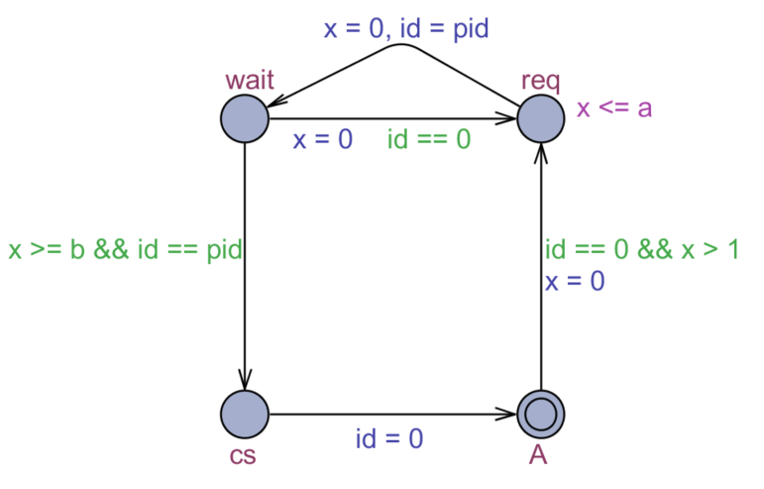
\includegraphics[width=80mm, keepaspectratio]{src/figures/fischer-uppaal.png}
    \caption{A Fischer-protokoll sablon automatája UPPAAL-ban}
    \label{fig:fischer-uppaal}
\end{figure}

\subsection{XTA formalizmus}
Az \ref{UPPAALmodell}. fejezetben bemutatott rendszert a következő XTA fájlba menti az UPPAAL:

\begin{verbatim}
const int N = 2;

typedef int[1, N] id_t;
int id;

process P(const id_t pid) {
clock x;
	const int a = 32;
	const int b = 64;
state
    wait,
    req {x <= a},
    A,
    cs;
init A;
trans
    A -> req { guard id == 0 && x > 1; assign x = 0;  },
    req -> wait { assign x = 0, id = pid;  },
    wait -> req { guard id == 0; assign x = 0;  },
    wait -> cs { guard x >= b && id == pid;  },
    cs -> A { assign id = 0;  };
}
system P;
\end{verbatim}

\subsection{ARG}
A modellből a Theta modellellenőrzője által felépített ARG egy részlete látható az \ref{fig:fischer-arg-reszlet} ábrán, a szaggatott élek az egymást fedő csúcsokat jelölik. (A teljes, 27 csúcsú ARG-t ábrázoló kép akkora, hogy teljesen olvashatatlan lenne.)

\begin{figure}%[h!]
    \centering
    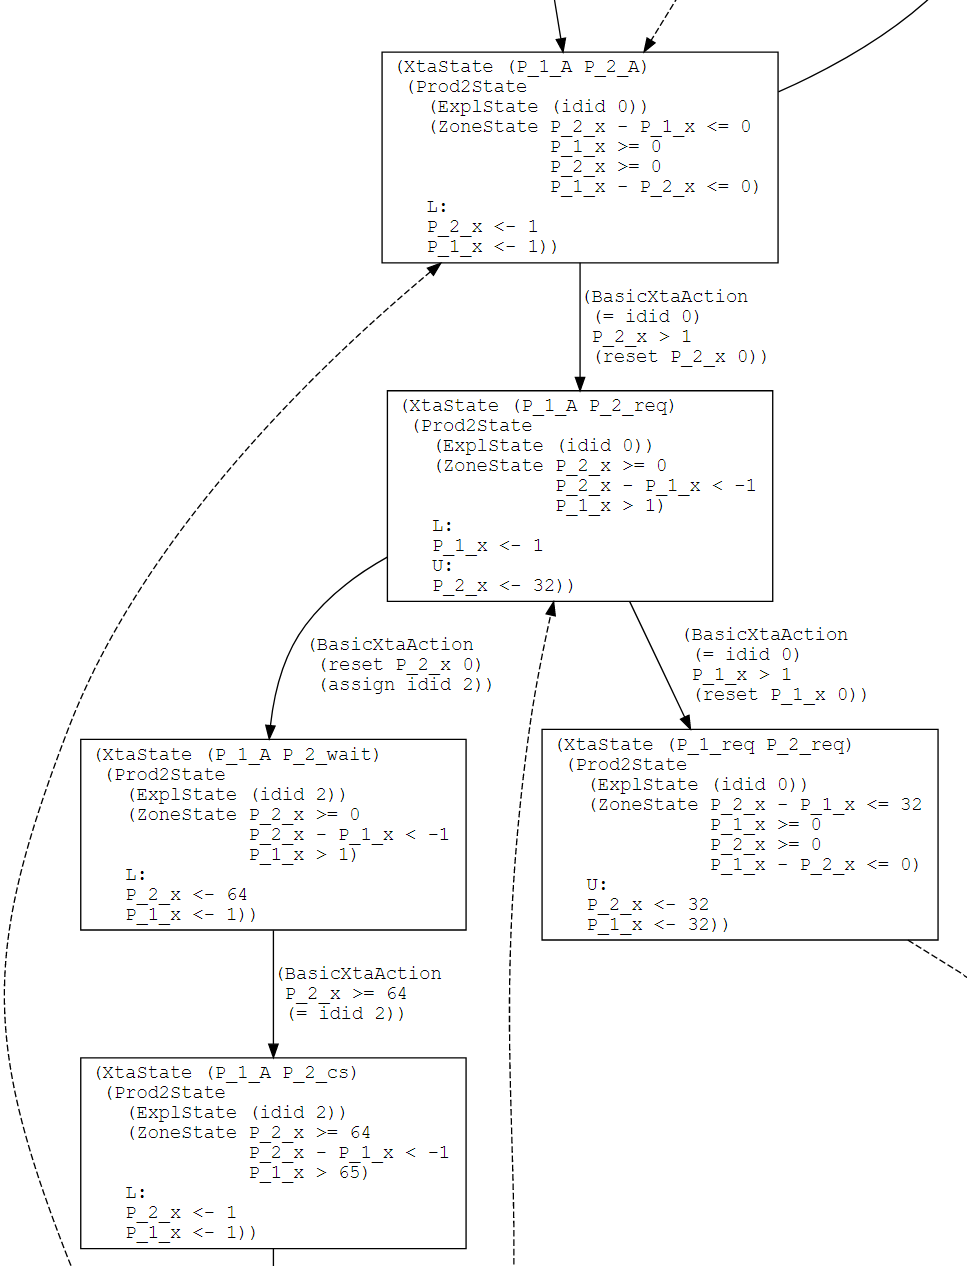
\includegraphics[width=\textwidth, keepaspectratio]{src/figures/fischer-arg-reszlet.png}
    \caption{A kétfolyamatú Fischer-protokoll ARG-jének részlete}
    \label{fig:fischer-arg-reszlet}
\end{figure}

\subsection{Tesztkészlet}

A kétfolyamatú modell összesen 8 vezérlési helyét a tesztgeneráló algoritmus 2 tesztesettel lefedte, ezek láthatók az \ref{fig:fischer-tests}. ábrán.

Megfigyelhető, hogy az \ref{fig:fischer-test1} ábrán látható teszteseten csak a \texttt{P\_1} automata lép, míg a \ref{fig:fischer-test2} ábrán láthatón csak \texttt{P\_2}.

A tört \texttt{delay} értékek magyarázata az \texttt{A} vezérlési helyről \texttt{req} vezérlési helyre vezető élen lévő \texttt{x > 1} őrfeltétel, amely kifejezésnek nincs minimális megoldása.

A tesztesetek szöveges leírása \aref{fig:fischer-tests-text}. ábrán látható.

\begin{figure}
\centering
\begin{minipage}{0.49\textwidth}
{\small \begin{verbatim}========== TRACE__7__P_1_cs ==========
(XtaState (P_1_A P_2_A)
  (Prod2State
    (ExplState (idid 0))
    (ZoneState P_2_x - P_1_x <= 0
               P_1_x >= 0
               P_2_x >= 0
               P_1_x - P_2_x <= 0)
    L:
    P_2_x <- 1
    P_1_x <- 1))
Delay: 1,484375
(BasicXtaAction
  (= idid 0)
  P_1_x > 1
  (reset P_1_x 0))
(XtaState (P_1_req P_2_A)
  (Prod2State
    (ExplState (idid 0))
    (ZoneState P_1_x - P_2_x < -1
               P_2_x > 1
               P_1_x >= 0)
    L:
    P_2_x <- 1
    U:
    P_1_x <- 32))
Delay: 0,000000
(BasicXtaAction
  (reset P_1_x 0)
  (assign idid 1))
(XtaState (P_1_wait P_2_A)
  (Prod2State
    (ExplState (idid 1))
    (ZoneState P_1_x - P_2_x < -1
               P_2_x > 1
               P_1_x >= 0)
    L:
    P_2_x <- 1
    P_1_x <- 64))
Delay: 64,000000
(BasicXtaAction
  (= idid 1)
  P_1_x >= 64)
(XtaState (P_1_cs P_2_A)
  (Prod2State
    (ExplState (idid 1))
    (ZoneState P_1_x - P_2_x < -1
               P_2_x > 65
               P_1_x >= 64)
    L:
    P_2_x <- 1
    P_1_x <- 1))
Delay: 0,000000
Total time: 65,484375
\end{verbatim}}
\subcaption{P\_1 vezérlési helyeit fedő teszteset}
\end{minipage}%
\hspace{0.01\textwidth}
\begin{minipage}{0.49\textwidth}%
%\centering
{\small \begin{verbatim}========== TRACE__10__P_2_cs ==========
(XtaState (P_1_A P_2_A)
  (Prod2State
    (ExplState (idid 0))
    (ZoneState P_2_x - P_1_x <= 0
               P_1_x >= 0
               P_2_x >= 0
               P_1_x - P_2_x <= 0)
    L:
    P_2_x <- 1
    P_1_x <- 1))
Delay: 1,500000
(BasicXtaAction
  (= idid 0)
  P_2_x > 1
  (reset P_2_x 0))
(XtaState (P_1_A P_2_req)
  (Prod2State
    (ExplState (idid 0))
    (ZoneState P_2_x >= 0
               P_2_x - P_1_x < -1
               P_1_x > 1)
    L:
    P_1_x <- 1
    U:
    P_2_x <- 32))
Delay: 0,000000
(BasicXtaAction
  (reset P_2_x 0)
  (assign idid 2))
(XtaState (P_1_A P_2_wait)
  (Prod2State
    (ExplState (idid 2))
    (ZoneState P_2_x >= 0
               P_2_x - P_1_x < -1
               P_1_x > 1)
    L:
    P_2_x <- 64
    P_1_x <- 1))
Delay: 64,000000
(BasicXtaAction
  P_2_x >= 64
  (= idid 2))
(XtaState (P_1_A P_2_cs)
  (Prod2State
    (ExplState (idid 2))
    (ZoneState P_2_x >= 64
               P_2_x - P_1_x < -1
               P_1_x > 65)
    L:
    P_2_x <- 1
    P_1_x <- 1))
Delay: 0,000000
Total time: 65,500000
\end{verbatim}}
\subcaption{P\_2 vezérlési helyeit fedő teszteset}
\end{minipage}
\caption{A kétfolyamatú Fischer-protokoll kettő tesztesete szövegesen}
\label{fig:fischer-tests-text}
\end{figure}

\begin{figure}
     \centering
     \begin{subfigure}[b]{0.4\textwidth}
         \centering
         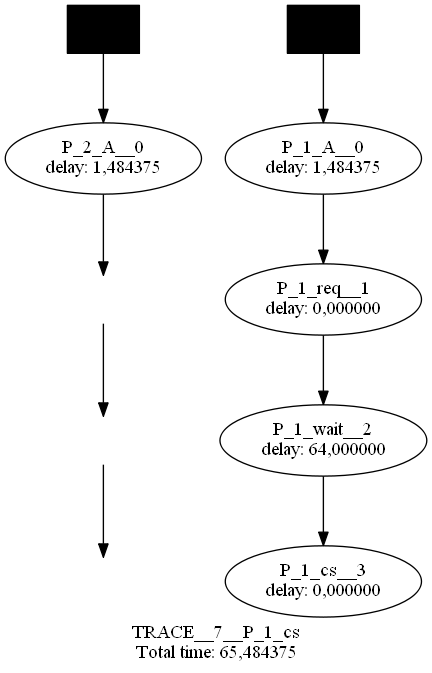
\includegraphics[width=\textwidth]{src/figures/fischer-test1.png}
         \caption{P\_1 vezérlési helyeit fedő teszteset}
         \label{fig:fischer-test1}
     \end{subfigure}
     \hfill
     \begin{subfigure}[b]{0.4\textwidth}
         \centering
         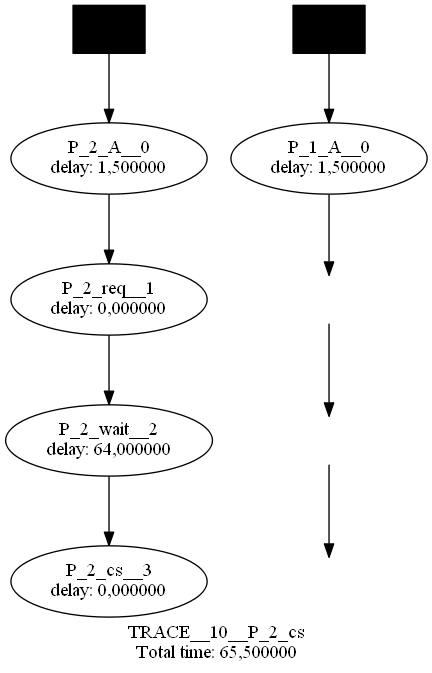
\includegraphics[width=\textwidth]{src/figures/fischer-test2.png}
         \caption{P\_2 vezérlési helyeit fedő teszteset}
         \label{fig:fischer-test2}
     \end{subfigure}
        \caption{A kétfolyamatú Fischer-protokoll kettő tesztesete grafikusan}
        \label{fig:fischer-tests}
\end{figure}

\section{Mérések} \label{meresek}

A bemutatott tesztgenerálási algoritmust számos XTA modellen lemértem. A mérések során a tesztgenerálás futásidejét, a generált tesztek számát, valamint a végső tesztkészlet elemszámát és a benne lévő tesztek összesített hosszát vizsgáltam.

A mérések során a Theta-t a \texttt{-{}-clock LU -{}-search BFS} paraméterekkel futtattam, minden tesztesetet 60 másodperces időkorláttal (ez az időkorlát nem a tesztgenerálásra, hanem a teljes futásra értendő). A méréseket Windows 10 operációs rendszeren végeztem, Intel Core i5-7200 processzorral, 8 GB RAM-mal. A mérési eredmények \aref{table:meresek}. táblázatban láthatók.

\begin{table}
\centering
\begin{tabular}{ |c||c|c||c|c|c|c| } 
 \hline
 \multirow{2}{*}{Modell} & \multicolumn{2}{c||}{ARG} & \multirow{2}{*}{\makecell{Futásidő \\ (ms)}} & \multirow{2}{*}{\makecell{Generált \\ tesztek}} & \multirow{2}{*}{$|\networktestset|$} & \multirow{2}{*}{$\sum{|\networktestset_i|}$} \\
  & mélység & méret & & & & \\
 
 \hline
critical-01-25-50.xta & 7 & 27 & 274 & 12 & 2 & 13 \\
critical-02-25-50.xta & 14 & 641 & 1723 & 85 & 4 & 28 \\
critical-03-25-50.xta & 22 & 21699 & 7623 & 410 & 6 & 45 \\
\hline
csma-01.xta & 2 & 3 & 509 & 2 & 1 & 2 \\
csma-02.xta & 5 & 21 & 353 & 9 & 2 & 7 \\
csma-03.xta & 8 & 99 & 1306 & 18 & 4 & 13 \\
csma-04.xta & 9 & 381 & 875 & 24 & 6 & 19 \\
csma-05.xta & 10 & 1272 & 1723 & 40 & 7 & 21 \\
csma-06.xta & 11 & 3865 & 2040 & 53 & 9 & 25 \\
csma-07.xta & 12 & 11008 & 4488 & 93 & 12 & 33 \\
csma-08.xta & 13 & 29925 & 4264 & 100 & 13 & 37 \\
csma-09.xta & 14 & 78552 & 4278 & 119 & 16 & 44 \\
\hline
fddi-001.xta & 9 & 15 & 813 & 11 & 2 & 15 \\
fddi-002.xta & 16 & 46 & 2144 & 26 & 3 & 34 \\
fddi-003.xta & 24 & 104 & 8495 & 48 & 4 & 60 \\
fddi-004.xta & 28 & 101 & 18073 & 62 & 4 & 74 \\
fddi-005.xta & 34 & 141 & 52396 & 85 & 4 & 89 \\
\arrayrulecolor{red}\hdashline\arrayrulecolor{black}
\textcolor{red}{fddi-006.xta} & \multicolumn{6}{c|}{\textcolor{red}{időtúllépés}} \\
\hline
fischer-01-32-64.xta & 4 & 5 & 152 & 4 & 1 & 4 \\
fischer-02-32-64.xta & 8 & 27 & 380 & 10 & 2 & 8 \\
fischer-03-32-64.xta & 10 & 121 & 508 & 20 & 3 & 12 \\
fischer-04-32-64.xta & 12 & 493 & 1083 & 35 & 4 & 16 \\
fischer-05-32-64.xta & 14 & 1911 & 1866 & 56 & 5 & 20 \\
fischer-06-32-64.xta & 16 & 7183 & 2648 & 79 & 6 & 24 \\
fischer-07-32-64.xta & 18 & 26405 & 3294 & 104 & 7 & 28 \\
fischer-08-32-64.xta & 20 & 95353 & 5829 & 165 & 8 & 32 \\
\hline
lynch-01-16.xta & 9 & 10 & 296 & 9 & 1 & 9 \\
lynch-02-16.xta & 13 & 61 & 867 & 30 & 2 & 18 \\
lynch-03-16.xta & 15 & 271 & 1716 & 76 & 3 & 27 \\
lynch-04-16.xta & 17 & 1049 & 4395 & 208 & 4 & 36 \\
lynch-05-16.xta & 19 & 3811 & 13247 & 582 & 5 & 45 \\
lynch-06-16.xta & 21 & 13453 & 39038 & 1490 & 6 & 54 \\
\arrayrulecolor{red}\hdashline\arrayrulecolor{black}
\textcolor{red}{lynch-07-16.xta} & \multicolumn{6}{c|}{\textcolor{red}{időtúllépés}} \\
\textcolor{red}{lynch-08-16.xta} & \multicolumn{6}{c|}{\textcolor{red}{időtúllépés}} \\
\hline
\end{tabular}
\caption{A tesztgenerálási algoritmus mérési eredményei}
\label{table:meresek}
\end{table}
% TeXstudio spellcheck 2020-12-10 16:40

\chapter{Összefoglalás} \label{osszefoglalas}

Szakdolgozatomban áttekintettem a modellellenőrzés alapjait, az időzített viselkedésmodellek leírására használt időzített automata formalizmust, valamint ennek bizonyos absztrakciós módszereit. Bemutattam az SMT problémákat és a Theta modellellenőrző keretrendszert.

Formalizáltam az időzített automaták hálózatain értelmezett valós idejű teszteket és tesztkészletet, majd az ezekre vonatkozó követelményeket. Kifejlesztettem egy algoritmust, amely minden vezérlési helyet lefedő tesztkészletet generál, majd a teszteseteket SMT problémaként megfogalmazva konkrét időzítéssel látja el. Megoldásomat implementáltam a Theta keretrendszer kiegészítéseként, amelyet szintén részletesen elemeztem.

Végül egy esettanulmányon keresztül részletesen is bemutattam a tesztgenerálási folyamatot, majd méréseket végeztem munkám értékelésére.

\section{Továbbfejlesztési lehetőségek} \label{tovabbfejlesztes}

Munkám elsődleges továbbfejlesztési lehetősége a generált tesztkészlettel szemben támasztott elvárásokkal kapcsolatos. A \ref{kovetelmenyek}. fejezetben bemutatott bizonyos elvárások ellentétben állhatnak egymással, például a tesztesetek számának és a tesztesetek hosszának minimalizálása. Adódik tehát az igény arra, hogy a tesztgeneráló algoritmust paraméterezni lehessen a követelmények priorizálásával.

A \ref{kovetelmenyek}. fejezetben bemutatottakon túl további elvárások is definiálhatók. Törekedhetünk például olyan tesztesetekre is, amelyek az állapotátmeneteket azok lehetséges időintervallumának a közepén vagy éppen a legszélén tüzelik. Előbbi esetben a teszt lefuttatása során kevésbé kell precíznek lenni az inputok időzítését illetően, míg utóbbi esetben ez a precizitás nélkülözhetetlen. Mindkettő lehet cél: előbbi esetben könnyebb a teszt lefuttatása, utóbbi esetben pedig tetten érhetünk nagyon kis valószínűséggel bekövetkező időzítési hibás eseteket.

Jelenleg a tesztesetek kimeneti formátuma szöveges és grafikus, vagyis közvetlenül nem futtathatók, munkám azonban további kimeneti formátumokkal is bővíthető. Amennyiben a teszteseteket az UPPAAL szimulátora által használt formátumban is előállítanám, azokat közvetlenül be lehetne tölteni az UPPAAL-ba, és ott szimulálhatóak lennének.

Nemcsak a tesztek szimulációja lehet cél, végső soron a konkrét rendszeren való futtatásuk is. Távlati célként megfogalmazható tehát a konkrét alkalmazás függvényében a tesztesetek tényleges előállítása.

% Acknowledgements
%~~~~~~~~~~~~~~~~~~~~~~~~~~~~~~~~~~~~~~~~~~~~~~~~~~~~~~~~~~~~~~~~~~~~~~~~~~~~~~~~~~~~~~
%----------------------------------------------------------------------------
\chapter*{\koszonetnyilvanitas}\addcontentsline{toc}{chapter}{\koszonetnyilvanitas}
%----------------------------------------------------------------------------

A szakdolgozat lelkes konzultálásán túl köszönöm konzulensemnek, Vincének, hogy 9.-es gimnazista koromtól délutáni szakkörökön megismertette és megszerettette velem a programozást, amely nélkül a szakdolgozatom talán egy másik szakon, más témában íródott volna.


% List of Figures, Tables
%~~~~~~~~~~~~~~~~~~~~~~~~~~~~~~~~~~~~~~~~~~~~~~~~~~~~~~~~~~~~~~~~~~~~~~~~~~~~~~~~~~~~~~
\listoffigures\addcontentsline{toc}{chapter}{\listfigurename}
\listoftables\addcontentsline{toc}{chapter}{\listtablename}
\listofalgorithms\addcontentsline{toc}{chapter}{\listalgorithmcfname}


% Bibliography
%~~~~~~~~~~~~~~~~~~~~~~~~~~~~~~~~~~~~~~~~~~~~~~~~~~~~~~~~~~~~~~~~~~~~~~~~~~~~~~~~~~~~~~

\bibliography{bib/mybib}
\addcontentsline{toc}{chapter}{\bibname}


% Appendix
%~~~~~~~~~~~~~~~~~~~~~~~~~~~~~~~~~~~~~~~~~~~~~~~~~~~~~~~~~~~~~~~~~~~~~~~~~~~~~~~~~~~~~~
%%----------------------------------------------------------------------------
\appendix
%----------------------------------------------------------------------------
\chapter*{\fuggelek}\addcontentsline{toc}{chapter}{\fuggelek}
\setcounter{chapter}{\appendixnumber}
%\setcounter{equation}{0} % a fofejezet-szamlalo az angol ABC 6. betuje (F) lesz
\numberwithin{equation}{section}
\numberwithin{figure}{section}
\numberwithin{lstlisting}{section}
%\numberwithin{tabular}{section}

%----------------------------------------------------------------------------
\section{A TeXstudio felülete}
%----------------------------------------------------------------------------
\begin{figure}[!ht]
\centering
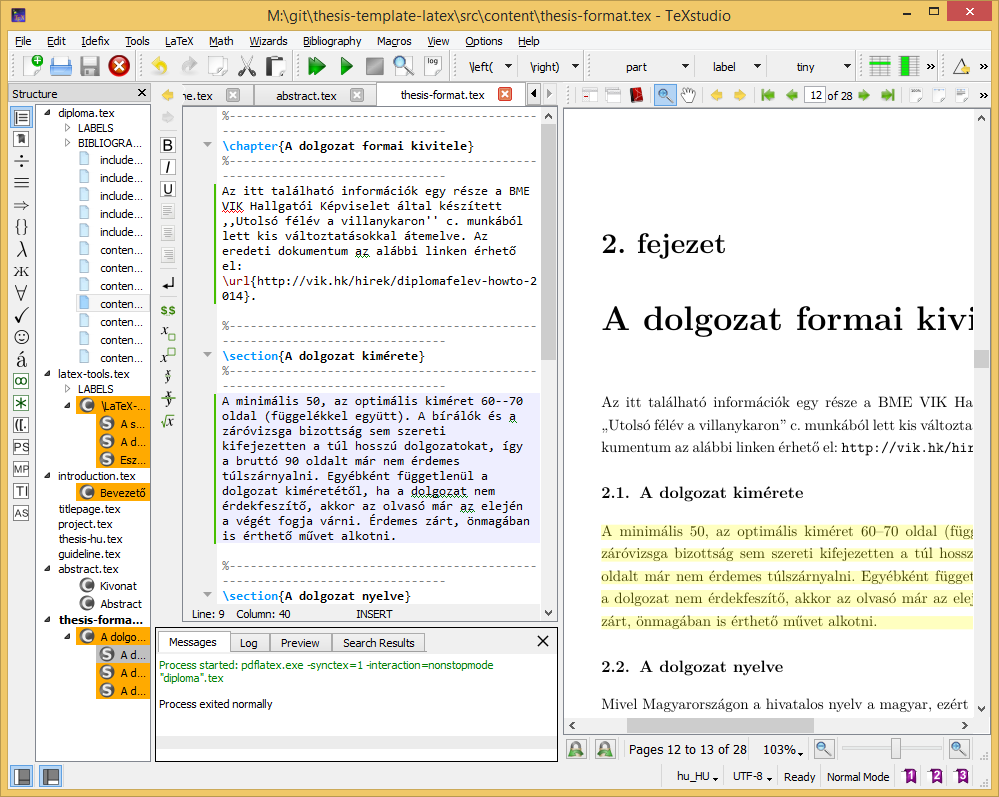
\includegraphics[width=150mm, keepaspectratio]{figures/TeXstudio.png}
\caption{A TeXstudio \LaTeX-szerkesztő.} 
\end{figure}

%----------------------------------------------------------------------------
\clearpage\section{Válasz az ,,Élet, a világmindenség, meg minden'' kérdésére}
%----------------------------------------------------------------------------
A Pitagorasz-tételből levezetve
\begin{align}
c^2=a^2+b^2=42.
\end{align}
A Faraday-indukciós törvényből levezetve
\begin{align}
\rot E=-\frac{dB}{dt}\hspace{1cm}\longrightarrow \hspace{1cm}
U_i=\oint\limits_\mathbf{L}{\mathbf{E}\mathbf{dl}}=-\frac{d}{dt}\int\limits_A{\mathbf{B}\mathbf{da}}=42.
\end{align}


%\label{page:last}
\end{document}
